\documentclass[11pt,letterpaper]{article}
\usepackage[margin=0.8in,headheight=15pt]{geometry}
\usepackage{fontspec}
\setmainfont{texgyrepagella}[Extension=.otf,UprightFont=*-regular,BoldFont=*-bold,ItalicFont=*-italic,BoldItalicFont=*-bolditalic]
\setsansfont{texgyreheros}[Extension=.otf,UprightFont=*-regular,BoldFont=*-bold,ItalicFont=*-italic,BoldItalicFont=*-bolditalic]
\usepackage{amsmath,amssymb,booktabs,tabularx,array,enumitem,xcolor}
\usepackage{graphicx}
\graphicspath{{units/ecology/book/assets/}{assets/}}
\usepackage{tikz}
\usetikzlibrary{arrows.meta,positioning,calc,decorations.pathmorphing,shapes.geometric}
\usepackage{fontawesome5}
\usepackage{wrapfig,multicol,needspace}
\usepackage{fancyhdr,hyperref}
\definecolor{forest}{HTML}{24594B}
\definecolor{pale}{HTML}{EFF5F1}
\definecolor{blue}{HTML}{305F82}
\definecolor{orange}{HTML}{9C5424}
\definecolor{leaf}{HTML}{4E8F3A}\definecolor{sunny}{HTML}{E0A526}\definecolor{soil}{HTML}{7A5A3A}\definecolor{fur}{HTML}{9C7B5B}\definecolor{sky}{HTML}{DCEBF5}\definecolor{heat}{HTML}{D2622A}\definecolor{coralc}{HTML}{D9736A}
\hypersetup{colorlinks=true,linkcolor=forest,urlcolor=blue,pdftitle={Shawn's Ecology Study Book 1A to 2C},pdfauthor={Prepared for Shawn}}
\pagestyle{fancy}\fancyhf{}
\fancyhead[L]{\small\sffamily SHAWN'S BIOLOGY}
\fancyhead[R]{\small\sffamily ECOLOGY\quad 1A--2C}
\fancyfoot[C]{\small\thepage}
\renewcommand{\headrulewidth}{0pt}
\setlength{\emergencystretch}{1em}
\setlength{\parindent}{0pt}\setlength{\parskip}{6pt}
\setlist[itemize]{leftmargin=1.3em,itemsep=3pt,topsep=3pt}
\setlist[enumerate]{leftmargin=1.6em,itemsep=6pt,topsep=3pt}
\renewcommand{\arraystretch}{1.24}
\newcolumntype{Y}{>{\raggedright\arraybackslash}X}
\newcommand{\pagechapter}[2]{\clearpage\section*{#1}\phantomsection\label{#2}\addcontentsline{toc}{section}{#1}}
\newcommand{\idea}[1]{\textbf{Main idea.} #1\par}
\newcommand{\term}[2]{\textbf{#1}: #2}
\newcommand{\memorycheck}[1]{\par\smallskip\textbf{Try from memory.} #1\par}
\newcommand{\source}[1]{{\footnotesize\textit{Further reading:} #1\par}}
\tikzset{concept/.style={draw=forest,fill=pale,rounded corners=3pt,align=center,font=\small\sffamily,text width=3.4cm,minimum height=1cm,inner sep=6pt}, flow/.style={-{Stealth[length=2.5mm]},thick,draw=forest}, rel/.style={font=\scriptsize\sffamily,fill=white,inner sep=2pt,align=center,text=black}}
\tikzset{cross/.style={-{Stealth[length=2.2mm]},thick,dashed,draw=black!55}, xrel/.style={rel,font=\scriptsize\sffamily,text width=2.3cm,inner sep=1pt,execute at begin node={\hyphenpenalty=10000\relax}}, drel/.style={rel,font=\scriptsize\sffamily,text width=,inner sep=1pt}}
% ---- pictogram system: Font Awesome 5 icons plus small editable TikZ drawings ----
\newcommand{\ico}[3][forest]{{\fontsize{#3}{#3}\selectfont\textcolor{#1}{#2}}}
\newcommand{\pn}[3]{\ico[#1]{#2}{19pt}\\[2pt]#3}
\tikzset{
 pics/rabbit/.style={code={
  \fill[#1] (0,0) ellipse (0.55 and 0.33);
  \fill[#1] (0.52,0.28) circle (0.23);
  \fill[#1,rotate around={12:(0.6,0.62)}] (0.6,0.62) ellipse (0.075 and 0.3);
  \fill[#1,rotate around={-14:(0.44,0.6)}] (0.44,0.6) ellipse (0.075 and 0.3);
  \fill[#1] (-0.56,0.08) circle (0.1);
  \fill[#1] (-0.25,-0.3) ellipse (0.17 and 0.09); \fill[#1] (0.25,-0.3) ellipse (0.17 and 0.09);
  \fill[white] (0.62,0.33) circle (0.04);}},
 pics/mushroom/.style={code={
  \fill[#1!80!black] (-0.12,0) rectangle (0.12,-0.42);
  \fill[#1] (-0.45,0) arc (180:0:0.45 and 0.36) -- cycle;
  \fill[white,opacity=0.85] (-0.17,0.14) circle (0.06) (0.14,0.1) circle (0.05) (0,0.26) circle (0.045);}},
 pics/grass/.style={code={
  \foreach \x/\h/\b in {-0.5/0.55/-0.15,-0.32/0.75/0.05,-0.12/0.6/-0.1,0.08/0.8/0.12,0.28/0.62/-0.05,0.48/0.5/0.1}{
   \fill[#1] (\x-0.06,0) .. controls (\x-0.03,\h*0.6) .. (\x+\b,\h) .. controls (\x+0.03,\h*0.6) .. (\x+0.06,0) -- cycle;}}},
 pics/soil/.style={code={
  \fill[soil!35,rounded corners=2pt] (-1,-0.45) rectangle (1,0.45);
  \foreach \p in {(-0.7,0.2),(-0.3,-0.2),(0.1,0.25),(0.5,-0.1),(0.8,0.2),(-0.5,-0.3),(0.3,0.05)} {\fill[soil] \p circle (0.05);}}},
 pics/sun/.style={code={
  \foreach \a in {0,45,...,315} {\draw[sunny,line width=1.4pt] (\a:0.42) -- (\a:0.6);}
  \fill[sunny] (0,0) circle (0.32);}},
 pics/road/.style={code={
  \fill[black!45] (-0.25,-#1) rectangle (0.25,#1);
  \foreach \y in {-1.3,-0.8,...,1.2} {\clip (-0.3,-#1) rectangle (0.3,#1); \fill[white] (-0.03,\y) rectangle (0.03,\y+0.28);}}},
 pics/coral/.style={code={
  \foreach \a/\l in {70/0.9,95/1.0,120/0.85,50/0.7,140/0.65} {\draw[#1,line width=3pt,line cap=round] (0,0) -- (\a:\l);}
  \foreach \a/\l/\b in {70/0.9/40,95/1.0/125,120/0.85/150,50/0.7/20} {\draw[#1,line width=2.2pt,line cap=round] (\a:\l*0.55) -- ++(\b:0.35);}}},
 heatarrow/.style={-{Stealth[length=2mm]},thick,draw=heat,decorate,decoration={snake,amplitude=0.6mm,segment length=2.6mm,post length=1.5mm}},
 lightarrow/.style={-{Stealth[length=2.5mm]},line width=1.2pt,draw=sunny},
 feed/.style={-{Stealth[length=2.5mm]},line width=1pt,draw=forest},
 gas/.style={-{Stealth[length=2.3mm]},thick,draw=blue},
 bubble/.style={circle,draw=blue,fill=sky,font=\small\sffamily,inner sep=2pt,minimum size=1cm},
 scene/.style={font=\footnotesize\sffamily,align=center,text=black,inner sep=2pt},
 pnode/.style={concept,text width=3.1cm,inner sep=6pt},
}
\newcommand{\vt}[3][forest]{\ico[#1]{#2}{10pt}\ \textbf{#3}}
\newenvironment{vocabtable}{\par\tabularx{\linewidth}{@{}>{\raggedright\arraybackslash}p{0.22\linewidth}Y >{\raggedright\arraybackslash}p{0.3\linewidth}@{}}\toprule Term & Meaning & Example or memory hook\\\midrule}{\bottomrule\endtabularx\par}
\newcommand{\academic}[2]{\subsection*{Academic words for this target}#1 These words are defined on page \pageref{#2}. Use them when you explain the biology terms above.\par}
\newcommand{\sq}[1]{\par\Needspace{6\baselineskip}\medskip{\color{forest}\textbf{Q.}}\ \textbf{#1}\par\smallskip}
\newcommand{\ans}[1]{#1\par}
\newcommand{\mc}[5]{\item #1\par\smallskip\begin{tabularx}{\linewidth}{@{}p{0.47\linewidth}p{0.47\linewidth}@{}}A.\ #2 & B.\ #3\\ C.\ #4 & D.\ #5\end{tabularx}\par}
\newcommand{\mcl}[5]{\item #1\par\smallskip A.\ #2\par B.\ #3\par C.\ #4\par D.\ #5\par}
\newcommand{\sumhead}[1]{\par\smallskip{\color{forest}\sffamily\bfseries #1}\par\nobreak\vspace{1pt}}
\newenvironment{sumlist}{\begin{itemize}[leftmargin=1.1em,itemsep=1pt,topsep=1pt,parsep=0pt]}{\end{itemize}}
\newcommand{\cb}{\raisebox{-1pt}{\large$\square$}}
\newcommand{\classsource}[1]{{\footnotesize\textit{Class connection:} #1\par}}
\makeatletter
\renewcommand{\l@section}{\@dottedtocline{1}{0em}{0em}}
\makeatother
\pdfstringdefDisableCommands{\def\quad{ }}
\begin{document}
\hypersetup{pageanchor=false}
\begin{titlepage}
\vspace*{0.7in}
{\sffamily\large BIOLOGY STUDY COLLECTION\par}
\vspace{0.35in}
{\Huge\bfseries Ecology\par}
\vspace{0.15in}
{\LARGE Knowledge and connections\par}
\vspace{0.25in}
{\Large Learning targets 1A through 2C\par}
\vspace{0.3in}
{\large Prepared for Shawn\par}
\vspace{0.5in}

\begin{tikzpicture}
\node[pnode] (a) at (0,0) {\pn{blue}{\faSearch}{Evidence}};
\node[pnode] (b) at (5.2,0) {\pn{leaf}{\faHeartbeat}{Living systems}};
\node[pnode] (c) at (10.4,0) {\pn{orange}{\faGlobeAmericas}{Ecological change}};
\draw[flow] (a)--node[rel,above]{explains}(b);
\draw[flow] (b)--node[rel,above]{respond to}(c);
\end{tikzpicture}\par
\vspace{0.45in}
This book connects scientific reasoning, homeostasis, energy and matter, biodiversity, and population ecology. Use the diagrams to explain relationships, then test your understanding with the questions at the end.

\textbf{Scope.} The teacher's \textit{Ecology Unit Guide} sets the learning targets. Shawn has covered 1A--2C. The supplied StudyBio practice quiz informs the review emphasis; it is not confirmation of the next exam's scope.

\textbf{How to use the book.} Read one section, close the book, and explain its main idea aloud. Redraw the related graph with labeled arrows. Attempt the review questions before checking the answers.
\vfill
{\small Original study explanations and diagrams supplement the teacher's outline. Class-specific policies and grading requirements must come from the class materials. Source notes and practice-key clarifications appear at the end.\par}
\end{titlepage}
\hypersetup{pageanchor=true}
{\setlength{\parskip}{0pt}\setlength{\columnsep}{18pt}\small\begin{multicols}{2}\tableofcontents\end{multicols}}
\vspace{12pt}
\textbf{Review sequence.} Each learning target opens with a vocabulary page; read it first, then return to it after the sections. Start with 1A and 1B, then connect metabolism to ecosystems in 1C. Use those ideas to explain biodiversity in 2A, human impacts in 2B, and population change in 2C.

\textbf{Before an exam.} Follow the seven-session study plan (page \pageref{plan}) and track yourself on the self-check (page \pageref{selfcheck}). The summary sheets (page \pageref{sumonea}), the model answers to the teacher's study questions (page \pageref{sqone}), and practice test A (page \pageref{testa}) are the last three steps.

\textbf{A useful answer has three parts:} name the concept, describe the mechanism, and apply the mechanism to the particular organism, ecosystem, or data.

\pagechapter{The knowledge graph}{graph}
\idea{Ecology connects mechanisms at different scales. Read each arrow as a sentence, not just a line between words.}
\begin{center}
\begin{tikzpicture}[x=1cm,y=1cm,concept/.append style={text width=4.6cm,minimum height=1.5cm,font=\sffamily,inner sep=8pt},rel/.append style={font=\footnotesize\sffamily}]
\node[concept] (a) at (0,0) {\pn{blue}{\faSearch}{\textbf{1A}\\Evidence and reasoning}};
\node[concept] (b) at (11.2,0) {\pn{heat}{\faHeartbeat}{\textbf{1B}\\Metabolism and homeostasis}};
\node[concept] (c) at (11.2,-4.9) {\pn{sunny}{\faSun\,\ico[forest]{\faRecycle}{19pt}}{\textbf{1C}\\Energy flow and matter cycling}};
\node[concept] (d) at (0,-4.9) {\pn{leaf}{\faTree}{\textbf{2A}\\Biodiversity and resilience}};
\node[concept] (e) at (0,-9.8) {\pn{black!65}{\faIndustry}{\textbf{2B}\\Human impacts and conservation}};
\node[concept] (f) at (11.2,-9.8) {\pn{orange}{\faChartLine}{\textbf{2C}\\Population size and limits}};
\draw[flow] (a)--node[rel,above]{tests explanations of}(b);
\draw[flow] (b)--node[rel,right,text width=3cm]{depend on energy\\and matter from}(c);
\draw[flow] (d)--node[rel,above]{can sustain ecosystem\\functions including}(c);
\draw[flow] (e)--node[rel,left,text width=3cm]{can reduce\\or protect}(d);
\draw[flow] (c)--node[rel,right,text width=3cm]{resource availability\\constrains}(f);
\draw[flow] (e)--node[rel,above]{alter habitats\\and resources for}(f);
\draw[flow] (a)--node[rel,left,text width=3cm]{evaluates claims\\about}(d);
\end{tikzpicture}\par
\end{center}
\textbf{Zoom in.} Use the next three mind maps for living systems (page \pageref{maplife}), energy and matter (page \pageref{mapenergy}), and ecological change (page \pageref{mapchange}). Then return here to connect the topics.
\subsection*{Three connections to explain}
\begin{enumerate}
\item \textbf{Organism to ecosystem:} cellular respiration supplies usable energy for homeostasis; food webs trace where the energy in an organism's food came from.
\item \textbf{Habitat to population:} habitat loss can reduce food and nesting sites, lowering carrying capacity and changing births, deaths, and movement.
\item \textbf{Biodiversity to resilience:} species that respond differently to disturbance can help ecosystem functions continue when one species declines.
\end{enumerate}
\memorycheck{Explain a path from human habitat change to a change in biodiversity, then to an ecosystem service people use.}

\pagechapter{Mind map: how we explain living systems}{maplife}
\idea{1A + 1B: begin with the central question, then follow each branch. Read an arrow together with the boxes it connects. Dashed arrows link one branch to another.}
\begin{center}
\begin{tikzpicture}[concept/.append style={text width=3.3cm,minimum height=1.1cm,font=\small\sffamily,execute at begin node={\hyphenpenalty=10000\relax}},rel/.append style={text width=3.2cm}]
\node[concept,fill=forest,text=white,text width=5.5cm] (root) at (6.2,0) {How do we explain living systems?};
\node[concept,draw=blue,fill=blue!10] (b0) at (0.0,-2.50) {\pn{blue}{\faSearch}{\textbf{Evidence and reasoning}}};
\draw[flow,draw=blue] (root.south)--++(0,-0.55)-|(b0.north);
\node[concept,draw=blue,fill=blue!5] (n00) at (0.0,-5.65) {\pn{blue}{\faEye}{Observations and measurements}};
\draw[flow,draw=blue] (b0)--node[rel]{begins with}(n00);
\node[concept,draw=blue,fill=blue!5] (n01) at (0.0,-8.80) {\pn{blue}{\faLightbulb}{Testable explanations}};
\draw[flow,draw=blue] (n00)--node[rel]{support or challenge}(n01);
\node[concept,draw=blue,fill=blue!5] (n02) at (0.0,-11.95) {\pn{blue}{\faFlask}{Predictions tested against new results}};
\draw[flow,draw=blue] (n01)--node[rel]{generate}(n02);
\node[concept,draw=forest,fill=forest!10] (b1) at (6.2,-2.50) {\pn{forest}{\faDna}{\textbf{Life and metabolism}}};
\draw[flow,draw=forest] (root.south)--++(0,-0.55)-|(b1.north);
\node[concept,draw=forest,fill=forest!5] (n10) at (6.2,-5.65) {\pn{forest}{\faMicroscope}{Cells and genetic information}};
\draw[flow,draw=forest] (b1)--node[rel]{depends on}(n10);
\node[concept,draw=forest,fill=forest!5] (n11) at (6.2,-8.80) {\pn{forest}{\faAtom}{Chemical reactions}};
\draw[flow,draw=forest] (n10)--node[rel]{organize}(n11);
\node[concept,draw=forest,fill=forest!5] (n12) at (6.2,-11.95) {\pn{forest}{\faSeedling}{Growth, repair, and cellular work}};
\draw[flow,draw=forest] (n11)--node[rel]{transfer energy for}(n12);
\node[concept,draw=orange,fill=orange!10] (b2) at (12.4,-2.50) {\pn{orange}{\faBalanceScale}{\textbf{Homeostasis}}};
\draw[flow,draw=orange] (root.south)--++(0,-0.55)-|(b2.north);
\node[concept,draw=orange,fill=orange!5] (n20) at (12.4,-5.65) {\pn{orange}{\faThermometerHalf}{Internal conditions within ranges}};
\draw[flow,draw=orange] (b2)--node[rel]{regulates}(n20);
\node[concept,draw=orange,fill=orange!5] (n21) at (12.4,-8.80) {\pn{orange}{\faSync*}{Feedback loops}};
\draw[flow,draw=orange] (n20)--node[rel]{uses responses in}(n21);
\node[concept,draw=orange,fill=orange!5] (n22) at (12.4,-11.95) {\pn{orange}{\faUndo}{Opposes the initiating change}};
\draw[flow,draw=orange] (n21)--node[rel]{negative feedback}(n22);
\draw[cross] (n01.east)--node[xrel,above]{propose mechanisms}(n11.west);
\draw[cross] (n11.east)--node[xrel,above]{power responses in}(n21.west);
\end{tikzpicture}\par
\end{center}
\par
\textbf{Connection to explain.} A person shivers when cold: temperature change is the stimulus; muscle activity uses ATP; metabolism releases heat; warming reduces the need to shiver. Evidence is needed to test each proposed relationship.
\par
\textbf{Common mix-up.} An observation records what was detected. An inference interprets it. Metabolism describes reactions; homeostasis describes regulation. Positive feedback amplifies change and needs an endpoint.
\par
\textbf{Close the book.} Draw three branches from memory. Explain how an experiment could test one response to a change in temperature.
\par
{\small Read more: reasoning, page \pageref{onea}; life, page \pageref{lifecheck}; feedback, page \pageref{feedback}.\par}
{\footnotesize Original study map synthesizing the class materials cited in the linked sections.\par}

\pagechapter{Mind map: energy flows and matter cycles}{mapenergy}
\idea{1C: begin with the central question, then follow each branch. Read an arrow together with the boxes it connects. Dashed arrows link one branch to another.}
\begin{center}
\begin{tikzpicture}[concept/.append style={text width=3.3cm,minimum height=1.1cm,font=\small\sffamily,execute at begin node={\hyphenpenalty=10000\relax}},rel/.append style={text width=3.2cm}]
\node[concept,fill=forest,text=white,text width=5.5cm] (root) at (6.2,0) {How does an ecosystem function?};
\node[concept,draw=blue,fill=blue!10] (b0) at (0.0,-2.50) {\pn{blue}{\faBolt}{\textbf{Energy enters}}};
\draw[flow,draw=blue] (root.south)--++(0,-0.55)-|(b0.north);
\node[concept,draw=blue,fill=blue!5] (n00) at (0.0,-5.65) {\pn{blue}{\faSun}{Sunlight}};
\draw[flow,draw=blue] (b0)--node[rel]{usually as}(n00);
\node[concept,draw=blue,fill=blue!5] (n01) at (0.0,-8.80) {\pn{blue}{\faSeedling}{Photosynthetic producers}};
\draw[flow,draw=blue] (n00)--node[rel]{captured by}(n01);
\node[concept,draw=blue,fill=blue!5] (n02) at (0.0,-11.95) {\pn{blue}{\faPaw}{Consumers and decomposers}};
\draw[flow,draw=blue] (n01)--node[rel]{supply food supporting}(n02);
\node[concept,draw=forest,fill=forest!10] (b1) at (6.2,-2.50) {\pn{forest}{\faMicroscope}{\textbf{Cells use energy}}};
\draw[flow,draw=forest] (root.south)--++(0,-0.55)-|(b1.north);
\node[concept,draw=forest,fill=forest!5] (n10) at (6.2,-5.65) {\pn{forest}{\faLungs}{Cellular respiration}};
\draw[flow,draw=forest] (b1)--node[rel]{through}(n10);
\node[concept,draw=forest,fill=forest!5] (n11) at (6.2,-8.80) {\pn{forest}{\faBatteryFull}{ATP}};
\draw[flow,draw=forest] (n10)--node[rel]{transfers fuel energy to}(n11);
\node[concept,draw=forest,fill=forest!5] (n12) at (6.2,-11.95) {\pn{forest}{\faRunning}{Movement, synthesis, and transport}};
\draw[flow,draw=forest] (n11)--node[rel]{powers}(n12);
\node[concept,draw=orange,fill=orange!10] (b2) at (12.4,-2.50) {\pn{orange}{\faRecycle}{\textbf{Matter is reused}}};
\draw[flow,draw=orange] (root.south)--++(0,-0.55)-|(b2.north);
\node[concept,draw=orange,fill=orange!5] (n20) at (12.4,-5.65) {\pn{orange}{\faBacteria}{Feeding, waste, and decomposition}};
\draw[flow,draw=orange] (b2)--node[rel]{through}(n20);
\node[concept,draw=orange,fill=orange!5] (n21) at (12.4,-8.80) {\pn{orange}{\faAtom}{Atoms and nutrients}};
\draw[flow,draw=orange] (n20)--node[rel]{move and rearrange}(n21);
\node[concept,draw=orange,fill=orange!5] (n22) at (12.4,-11.95) {\pn{orange}{\faLeaf}{Producers again}};
\draw[flow,draw=orange] (n21)--node[rel]{can be taken up by}(n22);
\draw[cross] (n01.north east)--node[drel,sloped,above]{also carry out}(n10.south west);
\draw[cross] (n10.south east)--node[drel,sloped,above]{returns CO$_2$ and water to}(n21.north west);
\draw[cross] (n02.east)--node[xrel,above]{use ATP for}(n12.west);
\end{tikzpicture}\par
\end{center}
\par
\textbf{Connect the branches.} Producers use light energy to build organic molecules. Feeding transfers those molecules and their energy. Producers, consumers, and decomposers use cellular metabolism and release heat.
\par
\textbf{Follow two different paths.} Food energy eventually dissipates as heat; atoms remain in matter and can be reused. Plants perform both photosynthesis and cellular respiration. Chemical energy supports chemosynthetic producers where sunlight is not the source.
\par
\textbf{Close the book.} Trace one carbon atom and one energy pathway through grass, a rabbit, and decomposers. Explain why the two paths do not have the same ending.
\par
{\small Read more: energy and matter, page \pageref{onec}; gas arrows, page \pageref{gases}; pyramids, page \pageref{pyramids}.\par}
{\footnotesize Original study map synthesizing the class materials cited in the linked sections.\par}

\pagechapter{Mind map: biodiversity, threats, and populations}{mapchange}
\idea{2A + 2B + 2C: begin with the central question, then follow each branch. Read an arrow together with the boxes it connects. Dashed arrows link one branch to another.}
\begin{center}
\begin{tikzpicture}[concept/.append style={text width=3.3cm,minimum height=1.1cm,font=\small\sffamily,execute at begin node={\hyphenpenalty=10000\relax}},rel/.append style={text width=3.2cm}]
\node[concept,fill=forest,text=white,text width=5.5cm] (root) at (6.2,0) {What changes an ecosystem?};
\node[concept,draw=blue,fill=blue!10] (b0) at (0.0,-2.50) {\pn{blue}{\faTree}{\textbf{Biodiversity}}};
\draw[flow,draw=blue] (root.south)--++(0,-0.55)-|(b0.north);
\node[concept,draw=blue,fill=blue!5] (n00) at (0.0,-5.65) {\pn{blue}{\faDna}{Genetic, species, and ecosystem diversity}};
\draw[flow,draw=blue] (b0)--node[rel]{includes}(n00);
\node[concept,draw=blue,fill=blue!5] (n01) at (0.0,-8.80) {\pn{blue}{\faShield*}{Resilience and ecosystem functions}};
\draw[flow,draw=blue] (n00)--node[rel]{can support}(n01);
\node[concept,draw=blue,fill=blue!5] (n02) at (0.0,-11.95) {\pn{blue}{\faHandHoldingWater}{Ecosystem services}};
\draw[flow,draw=blue] (n01)--node[rel]{benefit people as}(n02);
\node[concept,draw=forest,fill=forest!10] (b1) at (6.2,-2.50) {\pn{forest}{\faUsers}{\textbf{Human activities}}};
\draw[flow,draw=forest] (root.south)--++(0,-0.55)-|(b1.north);
\node[concept,draw=forest,fill=forest!5] (n10) at (6.2,-5.65) {\pn{forest}{\faExclamationTriangle}{CHIPPO threats}};
\draw[flow,draw=forest] (b1)--node[rel]{can create}(n10);
\node[concept,draw=forest,fill=forest!5] (n11) at (6.2,-8.80) {\pn{forest}{\faRoad}{Habitat quality and connectivity}};
\draw[flow,draw=forest] (n10)--node[rel]{can reduce}(n11);
\node[concept,draw=forest,fill=forest!5] (n12) at (6.2,-11.95) {\pn{forest}{\faHandsHelping}{Protection, restoration, and corridors}};
\draw[flow,draw=forest] (n11)--node[rel]{can improve through}(n12);
\node[concept,draw=orange,fill=orange!10] (b2) at (12.4,-2.50) {\pn{orange}{\faChartLine}{\textbf{Population change}}};
\draw[flow,draw=orange] (root.south)--++(0,-0.55)-|(b2.north);
\node[concept,draw=orange,fill=orange!5] (n20) at (12.4,-5.65) {\pn{orange}{\faExchange*}{Births + immigration versus deaths + emigration}};
\draw[flow,draw=orange] (b2)--node[rel]{depends on}(n20);
\node[concept,draw=orange,fill=orange!5] (n21) at (12.4,-8.80) {\pn{orange}{\faApple*}{Resources and limiting factors}};
\draw[flow,draw=orange] (n20)--node[rel]{interact with}(n21);
\node[concept,draw=orange,fill=orange!5] (n22) at (12.4,-11.95) {\pn{orange}{\faBalanceScale}{Carrying capacity and growth patterns}};
\draw[flow,draw=orange] (n21)--node[rel]{help determine}(n22);
\draw[cross] (n10.west)--node[xrel,above]{can reduce}(n00.east);
\draw[cross] (n11.east)--node[xrel,above]{help set}(n21.west);
\draw[cross] (n12.east)--node[xrel,above]{can raise}(n22.west);
\end{tikzpicture}\par
\end{center}
\par
\textbf{Read across the branches.} A road can remove habitat and isolate populations. Reduced resources can lower carrying capacity; isolation can reduce gene flow. A suitable crossing improves connectivity but does not solve every limiting factor.
\par
\textbf{Remember the qualifications.} Biodiversity can support resilience; it does not guarantee survival. Carrying capacity can change. An earlier Overshoot Day indicates greater demand relative to regeneration, not a direct species count.
\par
\textbf{Close the book.} Start with drought or habitat loss. Draw a chain connecting a limiting factor, population change, biodiversity, and one service used by people. Label uncertain outcomes with ``can.''
\par
{\small Read more: biodiversity, page \pageref{twoa}; CHIPPO, page \pageref{twob}; populations, page \pageref{twoc}; resources, page \pageref{resources}.\par}
{\footnotesize Original study map synthesizing the class materials cited in the linked sections.\par}


\pagechapter{Self-check\quad What I can do}{selfcheck}
\idea{Mark each statement honestly before you start and again after each study session. ``Yes'' means you can do it aloud, without notes, with an example. Study the ``not yet'' rows first.}
\par
{\small\renewcommand{\arraystretch}{1.08}\begin{tabularx}{\linewidth}{@{}p{0.06\linewidth}Y c c c@{}}\toprule
Target & I can\ldots & Not yet & Almost & Yes\\\midrule
1A & separate an observation from an inference and name a confounding factor & \cb & \cb & \cb\\
1A & explain induction and deduction with one example each and say how science uses both & \cb & \cb & \cb\\
1A & describe how the class grades work and what formative practice is for & \cb & \cb & \cb\\
1B & list the characteristics of life and apply them to fire, a seed, a mule, and a virus & \cb & \cb & \cb\\
1B & define metabolism and give building and breaking-down examples & \cb & \cb & \cb\\
1B & draw a negative feedback loop for temperature in both directions and explain why ``negative'' fits & \cb & \cb & \cb\\
1B & tell a control from a constant, and a hypothesis from a prediction & \cb & \cb & \cb\\
1C & define ecosystem, biotic, abiotic, habitat, and niche with examples & \cb & \cb & \cb\\
1C & draw a food web with correct arrow direction and name every role and trophic level & \cb & \cb & \cb\\
1C & write both equations and trace energy, oxygen, carbon dioxide, and heat through a web & \cb & \cb & \cb\\
1C & explain ``energy flows and matter cycles'' and use the 10\% rule in a calculation & \cb & \cb & \cb\\
1C & predict what happens when producers, decomposers, or top predators are removed & \cb & \cb & \cb\\
1C & give two reasons top predators are at risk, using the pyramid & \cb & \cb & \cb\\
2A & define biodiversity at three levels and explain why each matters & \cb & \cb & \cb\\
2A & name the four ecosystem service categories with an example and process for each & \cb & \cb & \cb\\
2A & explain the mechanism by which species diversity supports resilience & \cb & \cb & \cb\\
2B & expand CHIPPO and give a mechanism and a response for each threat & \cb & \cb & \cb\\
2B & explain how fragmentation lowers biodiversity and what a corridor can and cannot do & \cb & \cb & \cb\\
2B & write a CER with a specific claim, numerical evidence, and ``because'' reasoning & \cb & \cb & \cb\\
2C & calculate population change from births, deaths, immigration, and emigration & \cb & \cb & \cb\\
2C & sketch and explain J and S curves and name limiting factors of both kinds & \cb & \cb & \cb\\
2C & explain why populations fluctuate around $K$ and how $K$ changes & \cb & \cb & \cb\\
2C & explain Earth Overshoot Day, its formula, and why the date moves & \cb & \cb & \cb\\
2C & connect environmental justice to resource use with an example & \cb & \cb & \cb\\\bottomrule
\end{tabularx}}
\par
\textbf{Where to fix each row.} The vocabulary page, summary sheet, and model answers for the target, then the practice questions. Each statement matches one of the teacher's study questions (page \pageref{sqone}).

\pagechapter{Study plan\quad Seven sessions before the exam}{plan}
\idea{Each session takes 30 to 45 minutes. Start every session with five minutes of flashcards from the previous session, and end by updating the self-check on page \pageref{selfcheck}. Spread the sessions over at least a week; two sessions on one day are fine if they are hours apart.}
\par
\begin{tabularx}{\linewidth}{@{}p{0.1\linewidth}p{0.22\linewidth}Y@{}}\toprule
Session & Focus & What to do\\\midrule
1 & Orientation & Read the knowledge graph and three mind maps (pages \pageref{graph}--\pageref{mapchange}). Fill in the self-check honestly. Cut out the flashcards and sort them by target.\\
2 & 1A and 1B & Vocabulary pages, then the sections. Redraw both temperature loops from memory. Answer the 1A and 1B teacher questions aloud, then compare with page \pageref{sqone}.\\
3 & 1C & Vocabulary page, then the sections. Redraw the food web, the gas arrows, and the pyramid. Do review questions 5--9 (page \pageref{practiceone}) and check the answers.\\
4 & 2A and 2B & Vocabulary pages, then the sections. Write one CER with the template on page \pageref{certemplate} and score it with the rubric. Teacher questions for 2A and 2B.\\
5 & 2C & Vocabulary page, then the sections. Do the population equation and Overshoot Day calculations by hand. Sketch J and S curves and the lowered-$K$ graph. Teacher questions for 2C.\\
6 & Mixed retrieval & All flashcards, ``not yet'' pile twice. Review questions 10--20 and the diagram review (pages \pageref{practicetwo}--\pageref{diagrampractice}). Redraw one mind map from memory.\\
7 & Test rehearsal & Take practice test A (page \pageref{testa}) in 35 minutes, then grade with the key. Log every miss below. Restudy the weakest target with its summary sheet. Finish with the StudyBio blank quiz.\\\bottomrule
\end{tabularx}
\par
\textbf{If the exam date and scope arrive.} Ask the teacher which targets are covered, cross out anything outside the scope, and move session 7 to two days before the exam so there is time to restudy.
\subsection*{Mistake log}
Record every missed practice item. A pattern in the ``why'' column tells you what to fix.
\par
\begin{tabularx}{\linewidth}{@{}p{0.2\linewidth}p{0.08\linewidth}Y Y@{}}\toprule
Item (test or page) & Target & Why I missed it & What I will do differently\\\midrule
& & & \\[12pt]\midrule
& & & \\[12pt]\midrule
& & & \\[12pt]\midrule
& & & \\[12pt]\bottomrule
\end{tabularx}
\par
\pagechapter{1A\quad Vocabulary}{vocabonea}
\idea{Learn each term with its meaning and one example you can explain aloud. The page numbers show where the book uses the term.}
\begin{vocabtable}
\vt[blue]{\faEye}{Observation} & Information gathered directly with the senses or with instruments. & ``The leaf is 8 cm long.'' (page \pageref{onea})\\
\vt[sunny]{\faLightbulb}{Inference} & An interpretation or conclusion based on observations plus what you already know. & ``The plant may be short because it gets little light.''\\
\vt[forest]{\faChartLine}{Data} & Recorded observations or measurements used as evidence. & A table of seedling heights measured each week.\\
\vt[forest]{\faHashtag}{Quantitative data} & Data expressed as numbers, counts, or measurements. & 12 cm; 8 seedlings; 17 $^\circ$C\\
\vt[forest]{\faTag}{Qualitative data} & Data described in words or categories rather than numbers. & Yellow leaves; cloudy water.\\
\vt[blue]{\faSearch}{Induction} & Reasoning from many specific observations to a broader explanation. & Many shaded plants grow slowly, so shade may limit growth.\\
\vt[orange]{\faBullseye}{Deduction} & Reasoning from a general idea to a specific prediction that can be tested. & If light limits growth, plants given more light should grow taller.\\
\vt[orange]{\faEdit}{Annotation} & A note written on a text or diagram that marks a key idea, question, or connection. & Underlining \textit{carrying capacity} and writing ``changes with drought'' in the margin.\\
\vt[leaf]{\faClipboardCheck}{Formative assessment} & A low-stakes check used to guide learning and give feedback while you are still learning. & Homework, practice tests, and CFAs (page \pageref{classroom}).\\
\vt[leaf]{\faGraduationCap}{Summative assessment} & An assessment of what you have learned at the end of a unit or course. & The unit exam and the final exam.\\
\end{vocabtable}
\academic{Assess and assessment; collaboration; commitment; effective; feedback.}{vocab}
\memorycheck{Cover the meaning column and define each term aloud. Then turn one everyday sentence into a labeled observation and a labeled inference.}

\pagechapter{1A\quad Evidence and scientific reasoning}{onea}
\idea{Science builds explanations from observations, tests predictions, and revises explanations when evidence changes. Deliberate practice improves how clearly you do this.}
\subsection*{Distinctions to know}
\par
\begin{tabularx}{\linewidth}{@{}p{0.26\linewidth}Y@{}}\toprule
Concept & Meaning and example\\\midrule
Observation & What is measured or detected: ``The plant is 12 cm tall.''\\
Inference & An interpretation: ``The plant may be growing slowly because it receives little light.''\\
Quantitative data & Numerical measurements or counts, such as 12 cm or 8 seedlings.\\
Qualitative data & Descriptions, such as yellow leaves or cloudy water.\\
Induction & Particular observations lead to a broader explanation; repeated observations of shaded plants suggest a light--growth relationship.\\
Deduction & A general idea leads to a specific prediction: if light limits growth, otherwise similar plants given more light should grow more.\\\bottomrule
\end{tabularx}
\par
\subsection*{How the reasoning fits together}
An observation suggests a question. A testable explanation leads to a prediction. Measurements are compared with the prediction. Results can support an explanation, expose a weakness, or suggest a new question. One favorable result does not prove that an explanation is always true.

\textbf{Example.} A plant near a window is taller than a plant in a cupboard. The height difference is an observation. A claim that light caused the difference is an inference; water, species, and starting size could also differ.
\subsection*{Learning vocabulary}
\term{Annotation}{a note that identifies a key idea, question, or connection.}
\term{Formative assessment}{a check used to guide learning and feedback.}
\term{Summative assessment}{a check of achievement after a period of learning.}

Use \textbf{feedback} to identify a specific gap, practice the missing skill, and reassess. \textbf{Collaboration} includes comparing reasoning and explaining ideas; individual understanding still needs to be demonstrated.

\textbf{Class-specific information.} See page \pageref{classroom} for the supplied class expectations and grading overview.
\memorycheck{Change ``The pond is unhealthy'' into one measurable observation and one clearly labeled inference.}

\pagechapter{1A\quad Class expectations and scientific investigation}{classroom}
\idea{Use the learning targets to guide practice and the evidence to guide your conclusions.}
\subsection*{The assessment system in the class slides}
KUDOS provides the broad overview. The unit guide lists detailed vocabulary and study questions. Classwork, homework, notes, and review prepare students for the unit exams.
\par
\begin{tabularx}{\linewidth}{@{}p{0.26\linewidth}Y@{}}\toprule
Assessment & Supplied class policy\\\midrule
Formative practice & Homework, practice tests, and CFAs give feedback without directly affecting grades.\\
Checkups & 15\% of the grade; cover assigned work. Lowest two per semester dropped. No retake or makeup except for an excused absence.\\
Quality assignments & 20\% of the grade.\\
Quizzes and exams & 45\%. The unit exam can replace the quiz score. Exam retakes are available for scores below 80\%, with homework completion and a retake ticket required.\\
Final exam & 20\% of the grade.\\\bottomrule
\end{tabularx}\par
The slides estimate 15--30 minutes of focused homework nightly. If a student still struggles after more than an hour of focused work, they advise contacting the teacher and seeking tutorial help. These summarize the supplied deck; later teacher announcements may update policies.
\subsection*{Observations become testable explanations}
\begin{center}
\begin{tikzpicture}
\node[pnode] (o) at (0,0) {\pn{blue}{\faEye}{Observations and data}};
\node[pnode] (e) at (7.8,0) {\pn{sunny}{\faLightbulb}{General explanation}};
\node[pnode] (p) at (7.8,-3) {\pn{orange}{\faBullseye}{Specific prediction}};
\node[pnode] (t) at (0,-3) {\pn{forest}{\faFlask}{Test and compare}};
\draw[flow] (o)--node[rel,above]{induction suggests}(e);
\draw[flow] (e)--node[rel,right]{deduction yields}(p);
\draw[flow] (p)--node[rel,below]{guides measurements}(t);
\draw[flow] (t)--node[rel,left]{produces new}(o);
\end{tikzpicture}\par
\end{center}
A \textbf{hypothesis} is a testable proposed explanation. A \textbf{prediction} states a result expected if that explanation applies. Deduction guarantees a conclusion only with a valid argument and true premises; inductive conclusions remain revisable. Science uses both forms.
\textbf{Geotastic example.} A visible road sign is an observation; the inferred country is an interpretation. Comparing guessing error with the number of allowed advances can test a prediction, but player experience and location difficulty may also affect error.
\classsource{Biology Class Basics, slides 3--8; Deductive vs Inductive Reasoning Overview; Observation and Inference; Geotastic Inference Game.}


\pagechapter{1B\quad Vocabulary}{vocaboneb}
\idea{These terms describe what living things do and how scientists test explanations about them.}
\begin{vocabtable}
\vt[fur]{\faPaw}{Organism} & An individual living thing made of one or more cells. & A bacterium, a rabbit, or an oak tree.\\
\vt[heat]{\faFire}{Metabolism} & All the chemical reactions in an organism that build molecules or break them down, including those that transfer usable energy. & Photosynthesis and cellular respiration are metabolic processes (page \pageref{oneb}).\\
\vt[orange]{\faBalanceScale}{Homeostasis} & Keeping internal conditions within a working range even while the surroundings change. & Body temperature stays near 37 $^\circ$C in hot and cold weather.\\
\vt[blue]{\faAnchor}{Stable / stability} & Staying within a working range over time. Stable is not the same as constant. & A stable body temperature still rises and falls slightly.\\
\vt[orange]{\faSync*}{Feedback loop} & A cycle in which a change triggers a response, and the response then affects the original condition. & Temperature $\to$ sweating $\to$ temperature (page \pageref{feedback}).\\
\vt[orange]{\faUndo}{Negative feedback} & A response that opposes the initial change and brings the condition back toward its range. & Shivering when body temperature falls.\\
\vt[heat]{\faExpandArrows*}{Positive feedback} & A response that increases the initial change until something ends the loop. & Contractions during childbirth strengthen until delivery.\\
\vt[forest]{\faFlask}{Experimental control} & A comparison condition without the treatment, so you can see what happens on its own. & Bottle A with no hand in the energy-flow lab (page \pageref{lab}).\\
\vt[forest]{\faLock}{Constant} & A factor kept the same in every condition of an experiment. & The same volume of water in every bottle.\\
\vt[sunny]{\faLightbulb}{Hypothesis} & A testable proposed explanation. & ``Light limits the growth of these seedlings.''\\
\vt[orange]{\faBullseye}{Prediction} & The specific result expected if the hypothesis is correct. & ``Seedlings given more light will grow taller.''\\
\end{vocabtable}
\academic{Condition; constant; criteria; dynamic; equilibrium; mechanism; model; range; reinforce.}{vocab}
\memorycheck{Pick one condition your body regulates. Use \textit{stimulus}, \textit{response}, and \textit{negative feedback} correctly in three sentences about it.}

\pagechapter{1B\quad Life and homeostasis}{oneb}
\idea{Living organisms use matter and energy to maintain an organized, functioning system while conditions change.}
\subsection*{What makes a system alive}
An \textbf{organism} is an individual living system. Common characteristics of life include cellular organization, hereditary information, energy processing, regulation, responses to the environment, growth and development, and reproduction at the level of the life cycle or lineage. Populations evolve across generations. The full class checklist is explained on page \pageref{lifecheck}.

A single sign is not enough: a fire uses fuel and grows, but has no cells or inherited biological system. An individual that cannot reproduce can still be alive.
\subsection*{Metabolism and regulation}
\textbf{Metabolism} includes all chemical reactions that build or break down molecules. Photosynthesis builds organic molecules; cellular respiration transfers energy from fuel molecules to usable cellular forms; protein synthesis builds proteins from amino acids.

\textbf{Homeostasis} maintains internal conditions within a functional range. A stable range can include variation over time. It does not mean that an organism's interior matches the external environment or that every measurement remains exactly constant.
\begin{center}
\begin{tikzpicture}
\node[pnode] (a) at (0,0) {\pn{heat}{\faTemperatureHigh}{Temperature rises\\above its range}};
\node[pnode] (b) at (7.5,0) {\pn{black!70}{\faMale\,\ico[blue]{\faTint}{13pt}}{Cooling responses\\such as sweating}};
\node[pnode] (c) at (7.5,-3.2) {\pn{blue}{\faThermometerHalf}{Temperature decreases\\toward the range}};
\node[pnode] (d) at (0,-3.2) {\pn{black!60}{\faMinusCircle}{Cooling response\\is reduced}};
\draw[flow] (a)--node[rel,above]{triggers}(b);
\draw[flow] (b)--node[rel,right]{promote}(c);
\draw[flow] (c)--node[rel,below]{leads to}(d);
\end{tikzpicture}\par
\end{center}
\textbf{Negative feedback} opposes the initiating change. As temperature returns toward its regulated range, the corrective response is reduced. \textbf{Positive feedback} amplifies a change, as contractions promote signals that strengthen contractions during childbirth until delivery ends the loop. ``Positive'' and ``negative'' describe direction, not whether a response is helpful or harmful.

\textbf{Experimental control} provides a comparison condition. \textbf{Constants} are factors kept the same. In a temperature experiment, control food and water so their effects are not confused with temperature's effects.
\memorycheck{If temperature falls and shivering raises it, which feedback type is operating? Explain using the initial change and the response.}

\pagechapter{1B\quad The characteristics of life}{lifecheck}
\idea{A living organism is an organized cellular system. No single sign, such as movement or growth, is enough to identify life.}
\par
\begin{tabularx}{\linewidth}{@{}p{0.26\linewidth}Y@{}}\toprule
Characteristic & Meaning and a useful example\\\midrule
Made of cells & Cells are the basic units of life. A bacterium is unicellular; a tree is multicellular.\\
Reproduction & Organisms produce offspring through a life cycle or lineage. A sterile individual can still be alive.\\
Genetic information & DNA stores inherited information; RNA helps cells use that information. Offspring inherit information from parents.\\
Growth and development & Growth increases size or cell number. Development changes form or function, such as a seedling forming mature leaves.\\
Matter and energy use & Metabolic reactions supply materials and usable energy for cellular work. A plant takes in carbon dioxide and captures light energy.\\
Response to stimuli & A stimulus is a change an organism detects. A plant growing toward light is a response; walking is not required.\\
Homeostasis & Organisms regulate internal conditions within functional ranges even while the surroundings change.\\
Evolution & Inherited characteristics of populations change across generations. An individual does not evolve during its lifetime.\\\bottomrule
\end{tabularx}\par
\subsection*{Apply the whole checklist}
\textbf{Fire} spreads, uses fuel, and releases heat, but has no cells or biological genetic system. \textbf{A dormant seed} may show little visible activity, but contains living cells and can resume growth under suitable conditions. \textbf{A sterile mule} is alive despite its inability to reproduce.
\subsection*{Metabolism connects the characteristics}
Building molecules supports growth and repair. Breaking down fuel molecules can transfer energy to ATP. ATP supports movement, synthesis, and transport across membranes. These processes help cells maintain homeostasis.

\textbf{Do not confuse terms.} Metabolism is the collection of chemical reactions; homeostasis is regulation of conditions. Respiration is one metabolic process that helps supply energy for regulation. The class's example of a room warming when people enter connects cellular respiration to heat released into the surroundings.
\memorycheck{Explain why a feather is biologically derived material but is not itself a living organism.}
\classsource{Lecture 1 What Is Life Skeleton Notes; Metabolism, Trophic Levels and Energy Transfer, slides 2 and 5--7.}

\pagechapter{1B\quad Cells and viruses}{cells}
\idea{Viruses share genetic information and evolution with living systems, but lack the independent cellular organization used in the class's life checklist.}
\begin{center}
\begin{minipage}[c]{0.68\linewidth}
\centering\textbf{A bacterial cell}\par
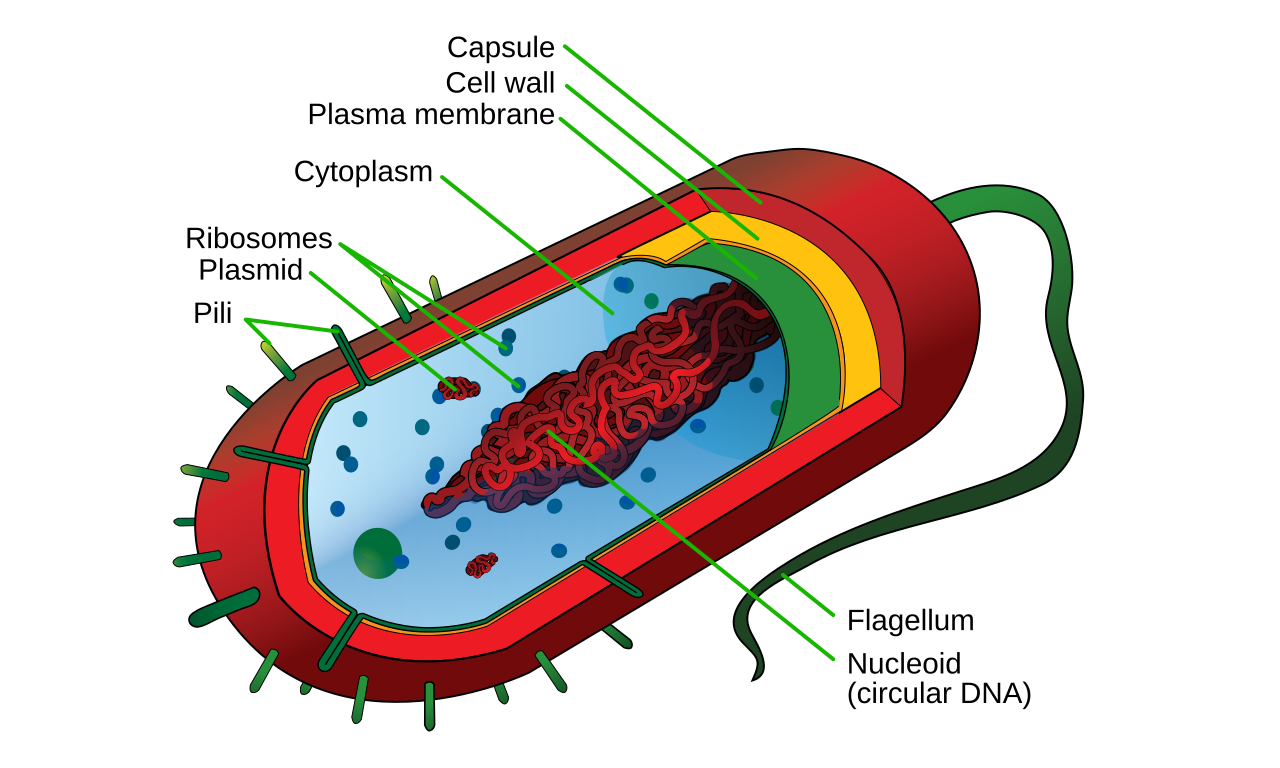
\includegraphics[width=0.9\linewidth]{bacterial-cell.png}
\end{minipage}\hfill
\begin{minipage}[c]{0.28\linewidth}
\centering\textbf{Adenovirus}\par

\includegraphics[width=\linewidth]{adenovirus.png}
\end{minipage}
\end{center}
{\small\textbf{Read the illustrations.} The bacterium has cytoplasm, ribosomes, and DNA in a nucleoid region, with no membrane-bound nucleus. The virus model shows the outer protein capsid and projecting fibers; its genome is inside and is not visible. These are illustrative models, not microscope photographs or a size comparison. Not all bacteria have every structure shown, and viruses have different shapes.\par}
{\footnotesize Cell: Mariana Ruiz Villarreal (LadyofHats), \href{https://commons.wikimedia.org/wiki/File:Average_prokaryote_cell-_en.svg}{Wikimedia Commons}, public domain. Virus: Thomas Splettstoesser, \href{https://commons.wikimedia.org/wiki/File:Adenovirus_3D_schematic.png}{Wikimedia Commons}, \href{https://creativecommons.org/licenses/by-sa/4.0/}{CC BY-SA 4.0}. Images reproduced without content changes; scaled for layout.\par}
\par
\begin{tabularx}{\linewidth}{@{}p{0.25\linewidth}Y Y@{}}\toprule
Feature & Cellular organism & Virus\\\midrule
Organization & One or more cells & Not made of cells\\
Genome & DNA & DNA or RNA\\
Metabolism & Has cellular metabolism & Lacks an independent metabolic system\\
Making copies & Uses cellular machinery & Requires a host cell's machinery\\
Evolution & Populations evolve & Viral populations evolve too\\\bottomrule
\end{tabularx}\par
\subsection*{How to answer the classification question}
State the criteria, then apply them. Under the usual school biology criteria, viruses are classified as nonliving because they are not cellular and cannot independently carry out metabolism or make new particles. Their genetic information and capacity to evolve explain why the comparison is interesting.

The viral coat helps protect the genome and, through viral surface structures, enables attachment to suitable host cells. A host cell supplies machinery and resources used to assemble new virus particles. A virus does not simply grow and divide like a cell.
\memorycheck{Why does requiring a host's cellular machinery matter more than simply requiring food from the environment?}
\classsource{Lecture 1 What Is Life Skeleton Notes, virus questions. Verification: \href{https://openstax.org/books/biology-2e/pages/21-introduction}{OpenStax Biology 2e, Viruses}.}

\pagechapter{1B\quad Drawing feedback loops}{feedback}
\idea{Track one measurable condition. Negative feedback opposes its change; positive feedback reinforces it. The sign describes a relationship, not whether a response is helpful.}
\subsection*{Temperature regulation in both directions}
\begin{center}
\begin{tikzpicture}
\node[pnode] (hot) at (0,0) {\pn{heat}{\faTemperatureHigh}{Temperature rises above its range}};
\node[pnode] (sweat) at (5.1,0) {\pn{black!70}{\faMale\,\ico[blue]{\faTint}{13pt}}{Sweating increases}};
\node[pnode] (down) at (10.2,0) {\pn{blue}{\faThermometerHalf}{Temperature decreases}};
\draw[flow] (hot)--node[rel,above]{triggers}(sweat);
\draw[flow] (sweat)--node[rel,above]{helps cause}(down);
\draw[flow] (down.south)--++(0,-0.8)-|node[rel,pos=0.25,below]{reduces further sweating}(sweat.south);
\node[pnode] (cold) at (0,-4.2) {\pn{blue}{\faTemperatureLow}{Temperature falls below its range}};
\node[pnode] (shiver) at (5.1,-4.2) {\pn{black!70}{\faMale\,\ico[blue]{\faSnowflake}{13pt}}{Shivering increases}};
\node[pnode] (up) at (10.2,-4.2) {\pn{heat}{\faThermometerHalf}{Temperature increases}};
\draw[flow] (cold)--node[rel,above]{triggers}(shiver);
\draw[flow] (shiver)--node[rel,above]{helps cause}(up);
\draw[flow] (up.south)--++(0,-0.8)-|node[rel,pos=0.25,below]{reduces further shivering}(shiver.south);
\end{tikzpicture}\par
\end{center}
Sweat evaporation transfers heat away from the body. Shivering uses repeated muscle contractions; greater energy use and metabolism release more heat. Recovery toward the regulated range reduces corrective action.
\subsection*{A self-reinforcing loop}
\begin{center}
\begin{tikzpicture}
\node[pnode] (p) at (0,0) {\pn{orange}{\faBaby}{Pressure on cervix}};
\node[pnode] (s) at (5.1,0) {\pn{orange}{\faBrain}{Signals promote oxytocin release}};
\node[pnode] (c) at (10.2,0) {\pn{orange}{\faHeartbeat}{Stronger uterine contractions}};
\draw[flow] (p)--node[rel,above]{triggers}(s);
\draw[flow] (s)--node[rel,above]{stimulates}(c);
\draw[flow] (c.south)--++(0,-0.8)-|node[rel,pos=0.3,below]{increase pressure, repeating the loop}(p.south);
\end{tikzpicture}\par
\end{center}
Delivery removes the initiating pressure. A chain that never returns to affect the original condition is not a complete feedback explanation.
\memorycheck{Choose an everyday condition, draw a response, and show how it changes the same condition.}
\classsource{Feedback Mechanisms and Homeostasis, slides 2--5; Feedback Mechanisms and Homestasis Practice.}


\pagechapter{1C\quad Vocabulary}{vocabonec}
\idea{Energy and matter words come in pairs. Learn each pair together and say what makes them different.}
\begin{vocabtable}
\vt[forest]{\faGlobeAmericas}{Ecosystem} & All the organisms in an area plus the nonliving environment and their interactions. & A pond: fish, plants, microbes, water, and sunlight (page \pageref{onec}).\\
\vt[leaf]{\faLeaf}{Biotic / abiotic} & Biotic: living or produced by living things. Abiotic: nonliving physical factors. & Biotic: frogs, dead leaves. Abiotic: temperature, water, light.\\
\vt[soil]{\faHome}{Habitat} & The place where an organism lives. & The pond is the frog's habitat.\\
\vt[blue]{\faPuzzlePiece}{Niche} & An organism's role: what it eats, what eats it, and the conditions and resources it uses. & Eating insects and being eaten by herons are parts of a frog's niche.\\
\vt[leaf]{\faSeedling}{Autotroph / producer} & Makes its own organic molecules from carbon dioxide using light or chemical energy. & Grass, algae, some bacteria.\\
\vt[fur]{\faPaw}{Heterotroph / consumer} & Gets organic matter and energy by eating other organisms or their products. & Rabbit, hawk, and mushroom.\\
\vt[blue]{\faBacteria}{Decomposer} & A heterotroph that breaks down dead organic matter and wastes, returning nutrients to soil or water. & Fungi and many bacteria (page \pageref{web}).\\
\vt[sunny]{\faSun}{Photosynthesis} & Producers use light energy to build sugar from carbon dioxide and water and release oxygen. & {\small $6\mathrm{CO_2}+6\mathrm{H_2O}+\text{light}$ \newline $\to\mathrm{C_6H_{12}O_6}+6\mathrm{O_2}$}\\
\vt[heat]{\faLungs}{Cellular respiration} & Cells break down sugar with oxygen, transferring energy to ATP and releasing carbon dioxide, water, and heat. & Happens in plants, animals, and decomposers (page \pageref{gases}).\\
\vt[forest]{\faRecycle}{Decomposition} & The breakdown of dead material into simpler substances by decomposers. & A fallen log rots; its nutrients return to the soil.\\
\vt[forest]{\faProjectDiagram}{Food web} & A diagram of feeding relationships. Each arrow points from the food to the eater. & Grass $\to$ rabbit $\to$ hawk (page \pageref{web}).\\
\vt[orange]{\faLayerGroup}{Trophic level} & An organism's feeding position in a food chain. & Producer, primary consumer, secondary consumer (p.\,\pageref{pyramids}).\\
\vt[forest]{\faBatteryFull}{ATP} & The molecule cells use as an immediate energy supply for work. & Muscle contraction uses ATP (p.\,\pageref{roles}).\\
\end{vocabtable}
\academic{Affect and effect; convert; cycle; efficient; generate; interact; obtain; population; process; release; store; transfer.}{vocab}
\memorycheck{Explain the difference within each pair: biotic and abiotic; habitat and niche.}

\pagechapter{1C\quad Energy and matter in ecosystems}{onec}
\idea{Energy passes through ecosystems and dissipates as heat. Matter is transferred and recycled through organisms and their surroundings.}
\subsection*{The parts of an ecosystem}
An \textbf{ecosystem} includes organisms, the physical environment, and their interactions. \textbf{Biotic} components involve life, including organisms and biologically derived material such as dead leaves in the class convention. \textbf{Abiotic} factors include temperature, light, humidity, water, and minerals.

A \textbf{habitat} is where an organism lives. Its \textbf{niche} includes how it uses resources, the conditions it tolerates, and its interactions. A pond is a frog's habitat; consuming insects and serving as prey are parts of its niche.
\par
\begin{tabularx}{\linewidth}{@{}p{0.28\linewidth}Y@{}}\toprule
Role & How matter and energy are obtained\\\midrule
Autotroph or producer & Builds organic molecules from inorganic carbon using light or chemical energy. Plants are familiar photosynthetic producers.\\
Heterotroph or consumer & Obtains organic matter from other organisms or their products. Animals, fungi, and many microbes are heterotrophs.\\
Decomposer & Breaks down dead organic material and wastes, returning nutrients to forms that can reenter ecosystem cycles. Many fungi and bacteria do this.\\\bottomrule
\end{tabularx}
\par
Most food webs rely on sunlight. Some producers use \textbf{chemosynthesis}, obtaining energy from chemical reactions involving inorganic substances rather than light. Lack of oxygen is not the defining feature.
\subsection*{Two processes to connect}
Simplified overall equations for oxygen-producing photosynthesis and aerobic cellular respiration are:
\begin{align*}
\text{Photosynthesis:}\quad 6\mathrm{CO_2}+6\mathrm{H_2O}+\text{light}
&\longrightarrow \mathrm{C_6H_{12}O_6}+6\mathrm{O_2}\\
\text{Respiration:}\quad \mathrm{C_6H_{12}O_6}+6\mathrm{O_2}
&\longrightarrow 6\mathrm{CO_2}+6\mathrm{H_2O}+\text{energy transfer}
\end{align*}
Photosynthesis stores transferred light energy in organic molecules. Respiration transfers chemical energy to ATP and releases heat. \textbf{Plants perform cellular respiration too.} ATP supports cellular work, including processes needed for homeostasis.

Atoms are rearranged in these reactions; energy is not turned into matter, and matter does not disappear into energy. Decomposers also metabolize and respire; they do not recycle heat into sunlight.
\memorycheck{Trace one carbon atom and the energy associated with food through a plant, a rabbit, and a decomposer. How do their paths differ?}

\pagechapter{1C\quad Reading a food web}{web}
\idea{A food-web arrow points from a food source to the organism receiving its matter and chemical energy.}
\begin{center}
\begin{tikzpicture}[x=1cm,y=1cm]
\node[scene] (sun) at (0.9,5.3) {\tikz{\pic{sun}}\\Sunlight};
\node[scene] (grass) at (0.9,2.2) {\tikz{\pic{grass=leaf}}\\Grass\\producer};
\node[scene] (rabbit) at (5.4,3.9) {\tikz{\pic{rabbit=fur}}\\Rabbit\\primary consumer};
\node[scene] (insect) at (5.4,0.8) {\ico[soil]{\faBug}{26pt}\\Grasshopper\\primary consumer};
\node[scene] (hawk) at (10.6,4.5) {\ico[black!70]{\faCrow}{30pt}\\Hawk\\predator};
\node[scene] (frog) at (10.6,1.3) {\ico[leaf!70!black]{\faFrog}{28pt}\\Frog\\secondary consumer};
\node[scene] (dead) at (5.4,-1.9) {\ico[soil]{\faLeaf}{22pt}\,\ico[black!55]{\faSkullCrossbones}{18pt}\\Dead material\\and waste};
\node[scene] (dec) at (10.6,-1.9) {\tikz{\pic{mushroom=orange!70!white}}\,\ico[blue]{\faBacteria}{22pt}\\Decomposers\\fungi and bacteria};
\node[scene] (soilnode) at (0.9,-1.9) {\tikz{\pic{soil}}\\Soil nutrients};
\draw[lightarrow] (sun)--node[rel,right]{light energy}(grass);
\draw[feed] (grass)--(rabbit);
\draw[feed] (grass)--(insect);
\draw[feed] (rabbit)--(hawk);
\draw[feed] (insect)--(frog);
\draw[feed] (frog)--(hawk);
\draw[feed,draw=soil] (dead)--node[rel,above]{organic matter}(dec);
\draw[feed,draw=soil] (dec.south) -- ++(0,-0.6) -| node[rel,pos=0.25,below]{mineral nutrients returned}(soilnode.south);
\draw[feed,draw=soil] (soilnode)--node[rel,left]{taken up by}(grass);
\end{tikzpicture}\par
\end{center}
Green arrows show feeding: each points from the food to the eater. All organisms contribute dead material or waste to the brown decomposer pathway; those arrows are omitted for clarity. Other arrows state the process represented. All living groups release metabolic heat, which leaves the food web as usable energy decreases.

\textbf{Trophic level} means feeding position. The hawk is a secondary consumer when eating a rabbit and a tertiary consumer when eating a frog that ate a grasshopper. An organism can occupy more than one trophic level.
\subsection*{Predict a change by following the links}
\begin{itemize}
\item \textbf{Remove producers:} the food supply to herbivores declines, and effects pass to predators. Existing stored food or imported organic matter can delay the response.
\item \textbf{Remove decomposers:} dead material accumulates and nutrient recycling slows; producer growth can eventually be limited.
\item \textbf{Remove top predators:} some prey may increase and consume more of their food. The size and timing of the response depend on alternative prey, competition, and other limits.
\end{itemize}
\memorycheck{Why does removing frogs not guarantee an immediate hawk decline in this web? State an alternative food source and a remaining uncertainty.}

\pagechapter{1C\quad Diagramming energy and gases}{gases}
\idea{Separate energy transfers from gas exchange. Gases enter or leave the surroundings rather than passing along feeding arrows.}
\subsection*{Energy pathway}
\begin{center}
\begin{tikzpicture}[x=1cm,y=1cm]
\node[scene] (sun) at (0,0) {\tikz{\pic{sun}}\\Sunlight};
\node[scene] (plant) at (4.1,0) {\ico[leaf]{\faSeedling}{32pt}\\Producer};
\node[scene] (animal) at (8.2,0) {\tikz{\pic{rabbit=fur}}\\Consumer};
\node[scene] (decomp) at (12.3,0) {\tikz{\pic{mushroom=orange!70!white}}\,\ico[blue]{\faBacteria}{20pt}\\Decomposer};
\draw[lightarrow] (sun)--node[rel,above]{light}(plant);
\draw[feed] (plant)--node[rel,above]{food}(animal);
\draw[feed] (animal)--node[rel,above,text width=1.5cm]{remains\\and waste}(decomp);
\foreach \a in {plant,animal,decomp} {
\draw[heatarrow] (\a.south)--++(0,-1.2) node[below,scene,text width=2.8cm]{heat to surroundings};
}
\draw[flow,dashed] (plant.north)--++(0,1)-|node[rel,pos=0.3,above]{dead producers also feed decomposers}(decomp.north);
\end{tikzpicture}\par
\end{center}
Photosynthesis converts light to chemical energy. Feeding transfers organic molecules and their chemical energy. Cellular respiration transfers energy to ATP, while metabolic processes release heat. Decomposers receive remains from any trophic level.
\subsection*{Gas exchange with the surroundings}
\begin{center}
\begin{tikzpicture}[x=1cm,y=1cm]
\node[bubble] (co) at (0,0) {CO$_2$};
\node[scene] (photo) at (5.4,0) {\ico[leaf]{\faSeedling}{30pt}\\Photosynthesis\\in a producer};
\node[bubble] (ox) at (10.8,0) {O$_2$};
\draw[gas] (co)--node[rel,above]{taken in}(photo);
\draw[gas] (photo)--node[rel,above]{released}(ox);
\node[bubble] (ox2) at (0,-3) {O$_2$};
\node[scene] (resp) at (5.4,-3) {\tikz{\pic[scale=0.8]{rabbit=fur}}\;\ico[leaf]{\faSeedling}{18pt}\;\ico[blue]{\faBacteria}{16pt}\\Aerobic cellular respiration\\in animals, plants, and decomposers};
\node[bubble] (co2) at (10.8,-3) {CO$_2$};
\draw[gas] (ox2)--node[rel,above]{taken in}(resp);
\draw[gas] (resp)--node[rel,above]{released}(co2);
\node[rel,text=blue] at (0,0.85) {air};\node[rel,text=blue] at (10.8,0.85) {air};
\node[rel,text=blue] at (0,-2.15) {air};\node[rel,text=blue] at (10.8,-2.15) {air};
\end{tikzpicture}\par
\end{center}
The respiration row applies to plants, animals, and aerobic decomposers. Plants need both sets of gas arrows. Aquatic organisms may exchange dissolved gases with water rather than directly with air.
\textbf{Decomposition} acts on dead material; the decomposer uses its own metabolism. Some microbes use pathways without oxygen, so the aerobic row does not represent every microbe.
\memorycheck{Draw a plant, a rabbit, and aerobic decomposers. Add food, heat, and gas arrows for every relevant process.}
\classsource{Metabolism, Trophic Levels and Energy Transfer, slides 2--7 and 19--27; Energy, Ecosystems, and Ecology Part 1; Energy and Matter Language Guide.}

\pagechapter{1C\quad Consumer roles and energy language}{roles}
\idea{Feeding role describes how an organism obtains organic matter. Trophic level describes its position in a particular feeding pathway.}
\par
\begin{tabularx}{\linewidth}{@{}p{0.25\linewidth}Y Y@{}}\toprule
Role & Definition & Example\\\midrule
Herbivore & Eats plants or algae & Rabbit eating grass\\
Carnivore & Eats animals & Hawk eating a rabbit\\
Omnivore & Eats plant and animal material & Bear eating berries and fish\\
Scavenger & Consumes remains of dead animals & Vulture feeding on a carcass\\
Detritivore & Ingests small pieces of dead organic matter & Earthworm eating organic material in soil\\
Decomposer & Breaks down organic matter externally and absorbs products & Fungus growing on dead wood\\\bottomrule
\end{tabularx}\par
These categories can overlap. Detritivores physically process material; microbial decomposers chemically break it down and return nutrients to reusable forms. Decomposers are heterotrophs, not producers.
\subsection*{Trace the molecules and the energy separately}
\textbf{Digestion} breaks food into smaller molecules that can be absorbed. \textbf{Cellular respiration} processes fuel molecules in cells, transferring chemical energy to ATP. \textbf{ATP} provides an immediate energy supply for muscle contraction, molecule synthesis, and transport across membranes.

Plants obtain most of the carbon in their organic molecules from carbon dioxide. Fertilizer supplies mineral nutrients; it does not supply the sunlight captured in photosynthesis. Water and minerals contribute matter, while light supplies energy.

\textbf{Say:} organisms obtain, store, convert, transfer, or release energy. Avoid saying organisms create energy or that glucose simply becomes ATP. During respiration, energy is transferred to ATP while atoms from fuel molecules are rearranged into products.
\subsection*{Worked comparison}
A wood-burning stove and a person both use energy stored in organic matter and release heat. In the person, cellular pathways also transfer energy to ATP for regulated cellular work. The stove does not have cells, homeostasis, or biological reproduction.

Shivering connects the same ideas: muscle contraction uses ATP, metabolism supplies usable energy, and heat release helps raise body temperature. Increased metabolic rate means more reactions per unit time, not the creation of new energy.
\memorycheck{Why is a mushroom a heterotroph even though it never chases prey?}
\classsource{Metabolism, Trophic Levels and Energy Transfer, slides 12--20; Trophic Levels Skeleton Notes; Energy and Matter Language Guide and questions; Energy and Matter Practice Questions.}

\pagechapter{1C\quad The energy-flow lab}{lab}
\idea{Compare water-temperature changes across control, still-hand, and moving-hand conditions, then explain the energy pathway.}
\begin{center}
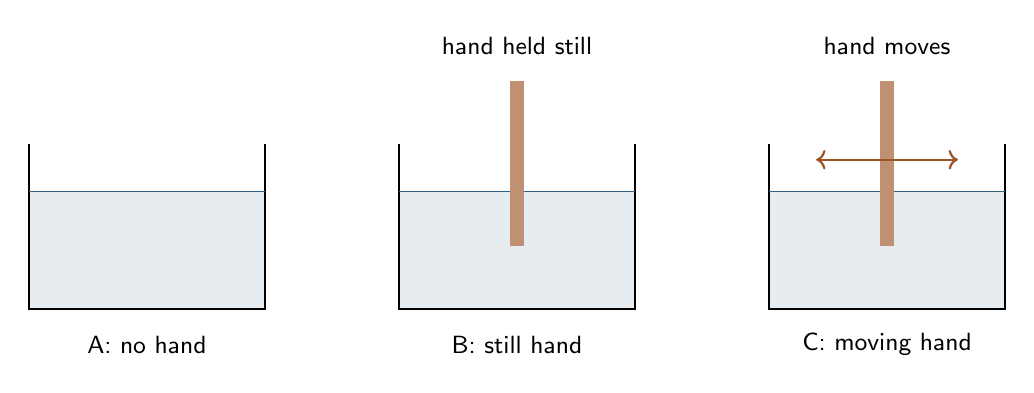
\begin{tikzpicture}[font=\small\sffamily]
\foreach \x/\lab in {0/A: no hand,4.7/B: still hand,9.4/C: moving hand} {
\fill[blue!12] (\x,0) rectangle ++(3,1.5);
\draw[thick] (\x,2.1)--(\x,0)--++(3,0)--++(0,2.1);
\draw[blue] (\x,1.5)--++(3,0);
\node at (\x+1.5,-0.45) {\lab};
}
\draw[line width=5pt,orange!65] (6.2,2.9)--(6.2,0.8);
\draw[line width=5pt,orange!65] (10.9,2.9)--(10.9,0.8);
\draw[<->,thick,orange] (10,1.9)--(11.8,1.9);
\node at (6.2,3.35) {hand held still};
\node at (10.9,3.35) {hand moves};
\end{tikzpicture}\par
\end{center}
\textit{Setup schematic.} Colored bars represent hands, not thermometers. The handout uses a 500-ml bottle of water for each container and records temperature initially and once each minute for five minutes.
\begin{center}
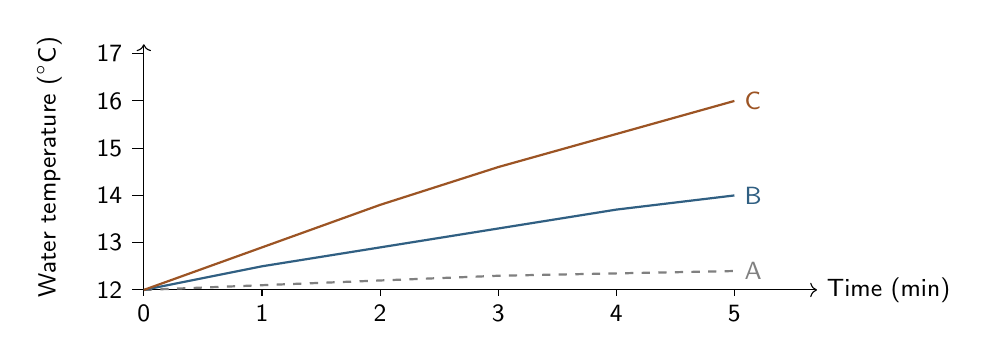
\begin{tikzpicture}[x=1.5cm,y=0.60cm,font=\small\sffamily]
\draw[->] (0,0)--(5.7,0) node[right]{Time (min)};
\draw[->] (0,0)--(0,5.2);
\node[rotate=90] at (-0.8,2.6) {Water temperature ($^\circ$C)};
\foreach \x in {0,1,2,3,4,5} {\draw (\x,0)--(\x,-0.12) node[below]{\x};}
\foreach \y/\lab in {0/12,1/13,2/14,3/15,4/16,5/17} {\draw (0,\y)--(-0.1,\y) node[left]{\lab};}
\draw[gray,thick,dashed] plot coordinates {(0,0)(1,0.1)(2,0.2)(3,0.3)(4,0.35)(5,0.4)} node[right]{A};
\draw[blue,thick] plot coordinates {(0,0)(1,0.5)(2,0.9)(3,1.3)(4,1.7)(5,2)} node[right]{B};
\draw[orange,thick] plot coordinates {(0,0)(1,0.9)(2,1.8)(3,2.6)(4,3.3)(5,4)} node[right]{C};
\end{tikzpicture}\par
\end{center}
\textbf{Invented practice data, not Shawn's results.} Changes are A: $0.4^\circ$C, B: $2.0^\circ$C, C: $4.0^\circ$C. A shows warming possible without a hand. Initial temperatures, hand size, movement, and timing are potential sources of variability.
\textbf{Heat calculation.} The handout's approximation for water is:
\[
Q\;(\mathrm{Cal})=V\;(\mathrm{L})\times\Delta T\;({}^\circ\mathrm C).
\]
For 0.50 L warmed by $4.0^\circ$C, $Q=2.0$ Cal, or 2 kcal. This is heat gained by the water, not all energy used by the body. Movement also affects mixing and heat transfer, so water warming does not isolate metabolic heat production.
\classsource{Energy Flow Lab 2021, procedure and quantitative questions; Energy and Matter Language Guide.}


\pagechapter{1C\quad Ecological pyramids}{pyramids}
\idea{Less energy is available to support production at successively higher trophic levels. This constrains food-chain length and predator populations.}
\begin{center}
\begin{tikzpicture}[x=1cm,y=1cm,font=\small\sffamily]
\fill[leaf!22] (-5.5,0) -- (5.5,0) -- (4.5,1.5) -- (-4.5,1.5) -- cycle;
\fill[fur!30] (-4.4,1.6) -- (4.4,1.6) -- (3.4,3.1) -- (-3.4,3.1) -- cycle;
\fill[forest!22] (-3.3,3.2) -- (3.3,3.2) -- (2.3,4.7) -- (-2.3,4.7) -- cycle;
\fill[black!15] (-2.2,4.8) -- (2.2,4.8) -- (1.2,6.3) -- (-1.2,6.3) -- cycle;
\node at (0,0.72) {\ico[leaf]{\faSeedling}{22pt}\;\ico[leaf]{\faSeedling}{22pt}\;\ico[leaf]{\faSeedling}{22pt}\;\ico[leaf]{\faSeedling}{22pt}\;\ico[leaf]{\faSeedling}{22pt}\;\ico[leaf]{\faSeedling}{22pt}};
\node at (0,2.3) {\tikz{\pic[scale=0.55]{rabbit=fur}}\;\tikz{\pic[scale=0.55]{rabbit=fur}}\;\ico[soil]{\faBug}{18pt}\;\ico[soil]{\faBug}{18pt}};
\node at (0,3.92) {\ico[leaf!70!black]{\faFrog}{22pt}\;\ico[leaf!70!black]{\faFrog}{22pt}};
\node at (0,5.55) {\ico[black!70]{\faCrow}{22pt}};
\node[anchor=east,align=right] at (-5.7,0.75) {Producers\\10,000 energy units};
\node[anchor=east,align=right] at (-4.6,2.35) {Primary consumers\\1,000};
\node[anchor=east,align=right] at (-3.5,3.95) {Secondary consumers\\100};
\node[anchor=east,align=right] at (-2.4,5.55) {Tertiary consumers\\10};
\foreach \x/\y in {5.05/0.75,4.05/2.35,2.95/3.95,1.85/5.55} {\draw[heatarrow] (\x+0.15,\y)--++(1.3,0) node[right,scene]{heat};}
\end{tikzpicture}\par
\end{center}
\textit{Illustration only:} values assume 10\% transfer at each step, use the same area and time interval, and are not measured data. Layer widths are schematic, not proportional to the numbers; the orange arrows show energy leaving each level as heat.

The \textbf{10\% rule} is a useful classroom approximation, not a fixed efficiency for every ecosystem. Energy not passed to the next consumer level can go into respiration and heat, uneaten material, or waste. Energy in detritus can still support decomposers before eventually dissipating as heat.
\[
E_{\text{next}}=E_{\text{current}}\times\text{transfer fraction}
\]
For an assumed 10\% transfer, two steps above 10,000 units gives
$10{,}000\times0.10\times0.10=100$ units.
\subsection*{Do not confuse three types of pyramid}
\begin{itemize}
\item \textbf{Energy:} energy transfer or production per area per time; an upright pattern is expected across a food chain.
\item \textbf{Biomass:} mass of organisms present; a snapshot can be inverted when rapidly reproducing producers are consumed quickly.
\item \textbf{Numbers:} count of organisms; one large tree can support many insects, so counts need not decrease at every level.
\end{itemize}
\subsection*{Why top predators are vulnerable}
\textbf{First,} limited energy supports relatively few predators, making small populations vulnerable to additional losses. \textbf{Second,} predators depend on a broad supporting prey base and often need large areas, making habitat loss and disruption below them consequential. \textbf{An additional risk} is biomagnification: some persistent pollutants reach higher concentrations up food chains.
\source{OpenStax, \href{https://openstax.org/books/biology-2e/pages/46-2-energy-flow-through-ecosystems}{Energy Flow through Ecosystems}, for pyramid exceptions and transfer efficiency.}
\memorycheck{Explain why ``the missing 90\% was destroyed'' is incorrect.}

\pagechapter{2A\quad Vocabulary}{vocabtwoa}
\idea{Biodiversity has levels, and its benefits have names. Match each term to the level or benefit it describes.}
\begin{vocabtable}
\vt[leaf]{\faTree}{Biodiversity} & The variety of life: genes within a species, species within a community, and ecosystems within a region. & The three-scale picture on page \pageref{diversity}.\\
\vt[blue]{\faDna}{Genetic diversity} & The variety of alleles within one species. & Rabbits of one species with different coat colors.\\
\vt[fur]{\faPaw}{Species diversity} & The number of species in a community and how evenly individuals are spread among them. & Five pollinator species sharing visits evenly.\\
\vt[forest]{\faMountain}{Ecosystem diversity} & The variety of ecosystems across a region. & Forest, wetland, and grassland in one county.\\
\vt[forest]{\faShield*}{Resilience} & The ability of an ecosystem to keep or recover its functions after a disturbance. & Pollination continues after drought because several pollinator species respond differently (page \pageref{twoa}).\\
\vt[blue]{\faHandHoldingWater}{Ecosystem services} & Benefits people get from ecosystems: provisioning, regulating, supporting, and cultural. & Food, clean water, crop pollination, and recreation.\\
\vt[sunny]{\faSpa}{Pollination} & Transfer of pollen to the receptive part of a flower, allowing fertilization and seed formation. & A bee carrying pollen between blossoms (page \pageref{cer}).\\
\vt[orange]{\faKey}{Keystone species} & A species whose effect on the community is large compared with its abundance. & A predator that keeps herbivores from overgrazing.\\
\vt[blue]{\faWater}{Foundation species} & A species that creates or defines the habitat that many others depend on. & Reef-building corals (page \pageref{diversity}).\\
\end{vocabtable}
\academic{Collapse; complex; context; diverse; dynamic; resilient; resources.}{vocab}
\memorycheck{For one ecosystem you know, name one example at each level of biodiversity and one service it provides to people.}

\pagechapter{2A\quad Biodiversity and ecosystem services}{twoa}
\idea{Variety within and among living systems can help ecosystem functions persist through change and provides benefits people rely on.}
\subsection*{Three scales of biodiversity}
\begin{itemize}
\item \textbf{Genetic diversity:} inherited variation within a species, such as different alleles affecting disease resistance.
\item \textbf{Species diversity:} variety of species in a community; both species richness and their relative abundances matter.
\item \textbf{Ecosystem diversity:} variety of ecosystems, such as wetlands, forests, and grasslands across a region.
\end{itemize}
\textbf{Resilience} is the capacity to recover or retain functions after disturbance. If several pollinators respond differently to drought, some may keep pollinating when others decline. Diversity often helps, but does not guarantee recovery from every disturbance. Species roles and the severity of change also matter.
\begin{center}
\begin{tikzpicture}
\node[pnode] (a) at (0,0) {\pn{leaf}{\ico[soil]{\faBug}{17pt}\,\ico[leaf!70!black]{\faFrog}{17pt}\,\ico[black!70]{\faCrow}{17pt}}{Different species\\and responses}};
\node[pnode] (b) at (7.5,0) {\pn{forest}{\faShield*}{Functions persist\\after disturbance}};
\node[pnode] (c) at (7.5,-3) {\pn{blue}{\faUsers}{Ecosystem services\\continue}};
\draw[flow] (a)--node[rel,above]{can allow}(b);
\draw[flow] (b)--node[rel,right]{help}(c);
\end{tikzpicture}\par
\end{center}
\subsection*{Ecosystem services are benefits to people}
Food, materials, water filtration, flood buffering, pollination, nutrient cycling, recreation, and cultural value connect ecosystem processes to human needs. \textbf{Pollination} transfers pollen to a receptive reproductive structure and enables fertilization in many plants.

The supplied Biodiversity Worksheet asks for all four categories, so learn each definition and be able to provide examples:
\par
\begin{tabularx}{\linewidth}{@{}p{0.25\linewidth}Y@{}}\toprule
Category & Examples\\\midrule
\ico[leaf]{\faTractor}{11pt}\ Provisioning & Food, timber, and other biological materials\\
\ico[blue]{\faTint}{11pt}\ Regulating & Flood moderation, water purification, crop pollination\\
\ico[forest]{\faRecycle}{11pt}\ Supporting & Nutrient cycling and soil formation\\
\ico[orange]{\faHiking}{11pt}\ Cultural & Recreation, scenic enjoyment, spiritual significance\\\bottomrule
\end{tabularx}
\par
\textbf{Keystone species.} A species whose effect on community structure is unusually large relative to its abundance. Some predators have this role, but not every predator is a keystone species.
\memorycheck{Explain how losing pollinators can affect plants, other animals, and humans.}

\pagechapter{2A\quad Seeing biodiversity at three scales}{diversity}
\idea{Genetic, species, and ecosystem diversity describe different levels. State which level your evidence measures.}
\begin{center}
\begin{tikzpicture}[font=\small\sffamily]
\foreach \x/\title in {0/Genetic diversity,4.7/Species diversity,9.4/Ecosystem diversity} {
\draw[forest,rounded corners] (\x,0) rectangle ++(4,2.7);
\node at (\x+2,3.05) {\title};
}
\pic[scale=0.6] at (0.9,1.9) {rabbit=fur}; \pic[scale=0.6] at (2.3,1.9) {rabbit=black!60}; \pic[scale=0.6] at (3.3,1.9) {rabbit=fur!45!white};
\node[font=\scriptsize\sffamily] at (0.9,1.0) {AA}; \node[font=\scriptsize\sffamily] at (2.3,1.0) {Aa}; \node[font=\scriptsize\sffamily] at (3.3,1.0) {aa};
\pic[scale=0.5] at (5.4,2.05) {rabbit=fur};
\node at (7.4,2.15) {\ico[black!70]{\faCrow}{20pt}};
\node at (5.6,0.8) {\ico[leaf!70!black]{\faFrog}{20pt}};
\node at (7.4,0.8) {\ico[soil]{\faBug}{18pt}};
\node at (8.1,1.5) {\ico[blue]{\faFish}{14pt}};
\fill[forest!30,rounded corners=2pt] (9.7,1.6) rectangle ++(1.5,1.1);
\fill[sky,rounded corners=2pt] (11.4,1.6) rectangle ++(1.6,1.1);
\fill[sunny!25,rounded corners=2pt] (9.7,0.3) rectangle ++(3.3,1.0);
\node at (10.45,2.15) {\ico[forest]{\faTree}{16pt}}; \node[font=\scriptsize\sffamily] at (10.45,1.72) {forest};
\node at (12.2,2.15) {\ico[blue]{\faWater}{16pt}}; \node[font=\scriptsize\sffamily] at (12.2,1.72) {wetland};
\pic[scale=0.55] at (10.25,0.42) {grass=leaf}; \pic[scale=0.55] at (12.55,0.42) {grass=leaf}; \node[font=\scriptsize\sffamily] at (11.4,0.55) {grassland};
\node[align=center,text width=4cm] at (2,-0.7) {Same species,\\different alleles};
\node[align=center,text width=4cm] at (6.7,-0.7) {Different species\\in one community};
\node[align=center,text width=4cm] at (11.4,-0.7) {Different habitats and\\ecological communities};
\end{tikzpicture}\par
\end{center}
The rabbits' coat colors and the letters beneath them represent schematic alleles, not complete genotypes. Genetic variation can increase the chance that some individuals tolerate a change. It cannot guarantee that a helpful trait exists or that every individual survives.
\subsection*{Why species roles matter}
A \textbf{keystone species} has an unusually large effect relative to its abundance. Some predators regulate prey and thereby influence vegetation and other organisms. The effect depends on the food web; not every predator is a keystone species.

The worksheet asks why corals matter. Reef-building corals create physical habitat used for shelter and feeding. Losing reef structure can affect many species. This habitat-building role is often described more precisely as a \textbf{foundation species} role.
\begin{center}
\begin{minipage}[c]{0.33\linewidth}
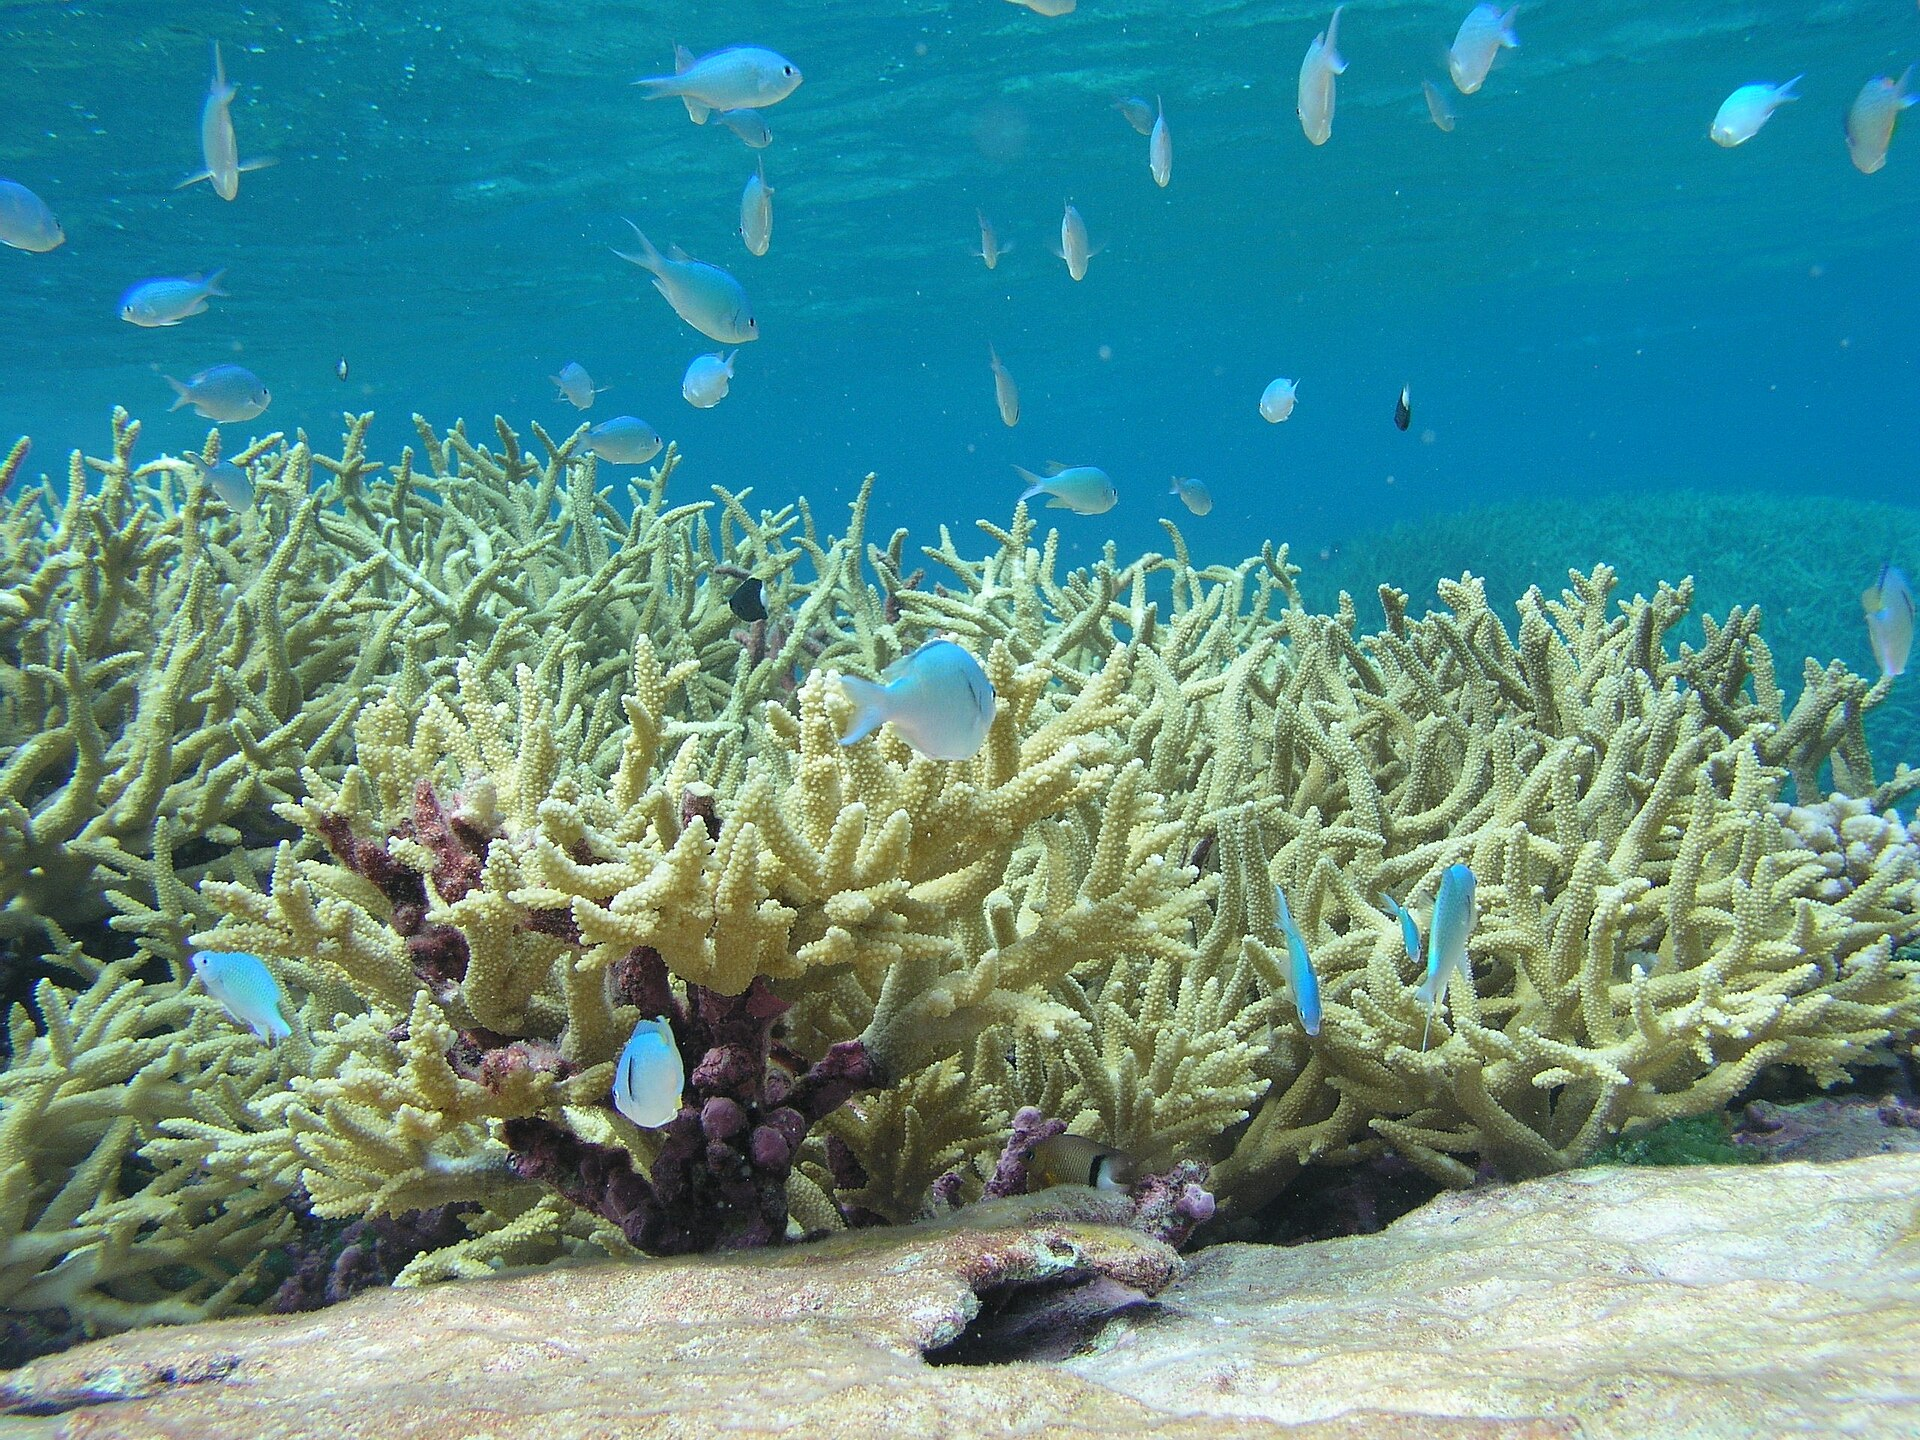
\includegraphics[width=\linewidth]{palmyra-reef.jpg}
{\footnotesize Chromis fish sheltering in staghorn coral, Palmyra Atoll. Amanda Meyer, USFWS, \href{https://commons.wikimedia.org/wiki/File:Chromis_reef_fish_and_staghorn_coral_at_Palmyra_Atoll_NWR_(5123997274).jpg}{Wikimedia Commons}, public domain.\par}
\end{minipage}\hfill
\begin{minipage}[c]{0.63\linewidth}
\begin{tikzpicture}[x=1cm,y=1cm,concept/.append style={text width=4.6cm,minimum height=0.9cm,inner sep=5pt,align=left}]
\node[concept] (c) at (0,0) {\tikz{\pic[scale=0.55]{coral=coralc};}\hspace{4pt}Reef-building corals};
\node[concept] (h) at (0,-1.7) {\ico[blue]{\faWater}{16pt}\hspace{6pt}Complex reef habitat};
\node[concept] (f) at (0,-3.4) {\ico[blue]{\faFish\,\faFish}{16pt}\hspace{6pt}Fish and invertebrate communities};
\draw[flow] (c)--node[rel,right]{build}(h);
\draw[flow] (h)--node[rel,right]{supports}(f);
\end{tikzpicture}\par
{\small The photo shows the middle step: coral branches are the shelter the fish use.\par}
\end{minipage}\par
\end{center}
\textbf{Services connect mechanisms to people.} Fish are provisioning resources; water purification is regulating; nutrient cycling is supporting; recreation and cultural meaning are cultural benefits. Explain both the category and the process.
\memorycheck{Does a forest with many trees, all of one species, necessarily have high tree species diversity?}
\classsource{Biodiversity Worksheet; Biodiversity and Its Threats Debrief, slides 2--6. Coral clarification: \href{https://coralreef.noaa.gov/digital-corals/visual-media/infographics/corals-are-important}{NOAA, Corals are Important}.}


\pagechapter{2B\quad Vocabulary}{vocabtwob}
\idea{These words name what people do to ecosystems and what can be done about it. Pair each threat with a response.}
\begin{vocabtable}
\vt[heat]{\faExclamationTriangle}{CHIPPO} & A memory aid for six threats: Climate change, Habitat loss, Invasive species, Pollution, Population, Overexploitation. & The table on page \pageref{twob} gives a response for each.\\
\vt[soil]{\faTractor}{Habitat loss} & Removal or degradation of the places organisms live. & A forest cleared for farmland.\\
\vt[black!60]{\faRoad}{Habitat fragmentation} & Division of habitat into separated patches, which limits movement and gene flow. & A highway splitting a forest (page \pageref{twob}).\\
\vt[soil]{\faBug}{Invasive species} & An introduced species that spreads and harms native species or ecosystems. & Not every introduced species is invasive; the harm matters.\\
\vt[blue]{\faFish}{Overexploitation} & Harvesting a population faster than it can replace its losses. & Overfishing a breeding population.\\
\vt[orange]{\faShoppingCart}{Overconsumption} & Using resources beyond what is needed or can be sustained. & Per-person use matters, not just the number of people.\\
\vt[heat]{\faExclamationCircle}{Endangered} & A species at high risk of extinction. & A small, isolated population losing habitat.\\
\vt[black!70]{\faSkullCrossbones}{Extinct} & No living individuals of the species remain. & Extinction cannot be reversed by conservation.\\
\vt[forest]{\faArrowsAltH}{Wildlife corridor} & A strip of habitat or a crossing that connects separated patches so organisms can move between them. & The Banff overpass (page \pageref{habitat}).\\
\vt[blue]{\faPen}{Claim, evidence, reasoning (CER)} & A claim answers the question; evidence is the data; reasoning explains how a scientific principle links them. & The flower-strip example on page \pageref{cer}.\\
\end{vocabtable}
\academic{Consumption; destroy and destruction; disrupt and disruption; exploit and exploitation; impact; migrate and migration; prevent and prevention; restore and restoration; threat and threaten.}{vocabtwo}
\memorycheck{Expand CHIPPO from memory. For two of the threats, state the mechanism of harm and one matching conservation response.}

\pagechapter{2B\quad Threats to biodiversity}{twob}
\idea{Human activities change habitats, resources, and interactions. Conservation works best when it addresses the specific cause of decline.}
The practice key expands \textbf{CHIPPO} as follows:
\par
\begin{tabularx}{\linewidth}{@{}p{0.25\linewidth}Y@{}}\toprule
Threat & Mechanism and a possible response\\\midrule
Climate change & Shifts temperature, rainfall, and habitat suitability. Reduce emissions and protect routes for species movement.\\
Habitat loss & Farming, buildings, roads, logging, and mining can remove or degrade habitat. Protect and restore suitable habitat.\\
Invasive species & Introduced species can spread and harm native species through competition, predation, or disease. Prevent introductions and manage established invasions.\\
Pollution & Chemicals, nutrient excess, plastics, and other pollutants can impair organisms or habitats. Reduce releases at their source.\\
Population & Human population size interacts with consumption and technology to influence resource demand. Improve access to resources and reduce waste and damaging demand.\\
Overexploitation & Harvest exceeds a population's capacity to replace losses. Use sustainable harvest limits and protect breeding populations.\\\bottomrule
\end{tabularx}
\par
\textbf{Overconsumption} means resource use beyond what is needed or can be sustained. Population alone does not determine impact: per-person use and production methods also matter. \textbf{Endangered} species face a high risk of extinction; an \textbf{extinct} species has no living individuals remaining.
\subsection*{Habitat loss versus fragmentation}
\textbf{Loss} reduces the amount of habitat. \textbf{Fragmentation} divides habitat into separated patches. The same development can do both. Isolation can limit migration and mating, reduce gene flow, increase edge exposure, and make local losses harder to reverse.
\begin{center}
\begin{tikzpicture}[x=1cm,y=1cm,font=\small\sffamily]
\begin{scope}
\fill[leaf!25,rounded corners=3pt] (0,0) rectangle (4.2,2.5);
\pic[scale=0.45] at (0.8,1.85) {rabbit=fur}; \pic[scale=0.45] at (2.2,1.2) {rabbit=fur}; \pic[scale=0.45] at (3.3,1.9) {rabbit=fur}; \pic[scale=0.45] at (1.2,0.6) {rabbit=fur};
\draw[{Stealth}-{Stealth},thick,forest] (0.6,1.25)--(3.6,1.25);
\node[align=center] at (2.1,-0.45) {Continuous habitat:\\free movement};
\end{scope}
\begin{scope}[xshift=5.6cm]
\fill[leaf!25,rounded corners=3pt] (0,0) rectangle (4.2,2.5);
\pic at (2.1,1.25) {road=1.25};
\node at (2.1,2.15) {\ico[black!70]{\faCar}{10pt}};
\pic[scale=0.45] at (0.8,1.85) {rabbit=fur}; \pic[scale=0.45] at (1.0,0.7) {rabbit=fur}; \pic[scale=0.45] at (3.3,1.9) {rabbit=fur};
\draw[-{Stealth},thick,forest] (0.6,1.25)--(1.75,1.25);
\node at (2.1,0.95) {\ico[red!70!black]{\faTimes}{13pt}};
\node[align=center] at (2.1,-0.45) {Road divides it:\\movement and gene flow drop};
\end{scope}
\begin{scope}[xshift=11.2cm]
\fill[leaf!25,rounded corners=3pt] (0,0) rectangle (4.2,2.5);
\pic at (2.1,1.25) {road=1.25};
\fill[leaf!60] (1.4,0.9) rectangle (2.8,1.6);
\node at (2.1,2.15) {\ico[black!70]{\faCar}{10pt}};
\pic[scale=0.45] at (0.8,1.85) {rabbit=fur}; \pic[scale=0.45] at (1.0,0.7) {rabbit=fur}; \pic[scale=0.45] at (3.3,1.9) {rabbit=fur};
\draw[{Stealth}-{Stealth},thick,forest] (0.6,1.25)--(3.6,1.25);
\node at (2.1,0.4) {\ico[forest]{\faCheck}{13pt}};
\node[align=center] at (2.1,-0.45) {Corridor added:\\movement returns; habitat still lost};
\end{scope}
\end{tikzpicture}\par
\end{center}
The green band over the road is a wildlife corridor. \textbf{Wildlife corridors} connect patches and can improve movement. Their benefits depend on design and species; connecting patches does not replace all lost habitat. An introduced species is not automatically invasive: harmful effects matter.\footnote{See \href{https://www.cbd.int/invasive}{Convention on Biological Diversity, Invasive Alien Species}.}
\memorycheck{For a road that splits a forest, explain one benefit of a wildlife crossing and one problem the crossing alone cannot solve.}

\pagechapter{2B\quad Habitat loss and corridors}{habitat}
\idea{Habitat amount and connectivity are different. Protecting one does not automatically protect the other.}
\begin{center}
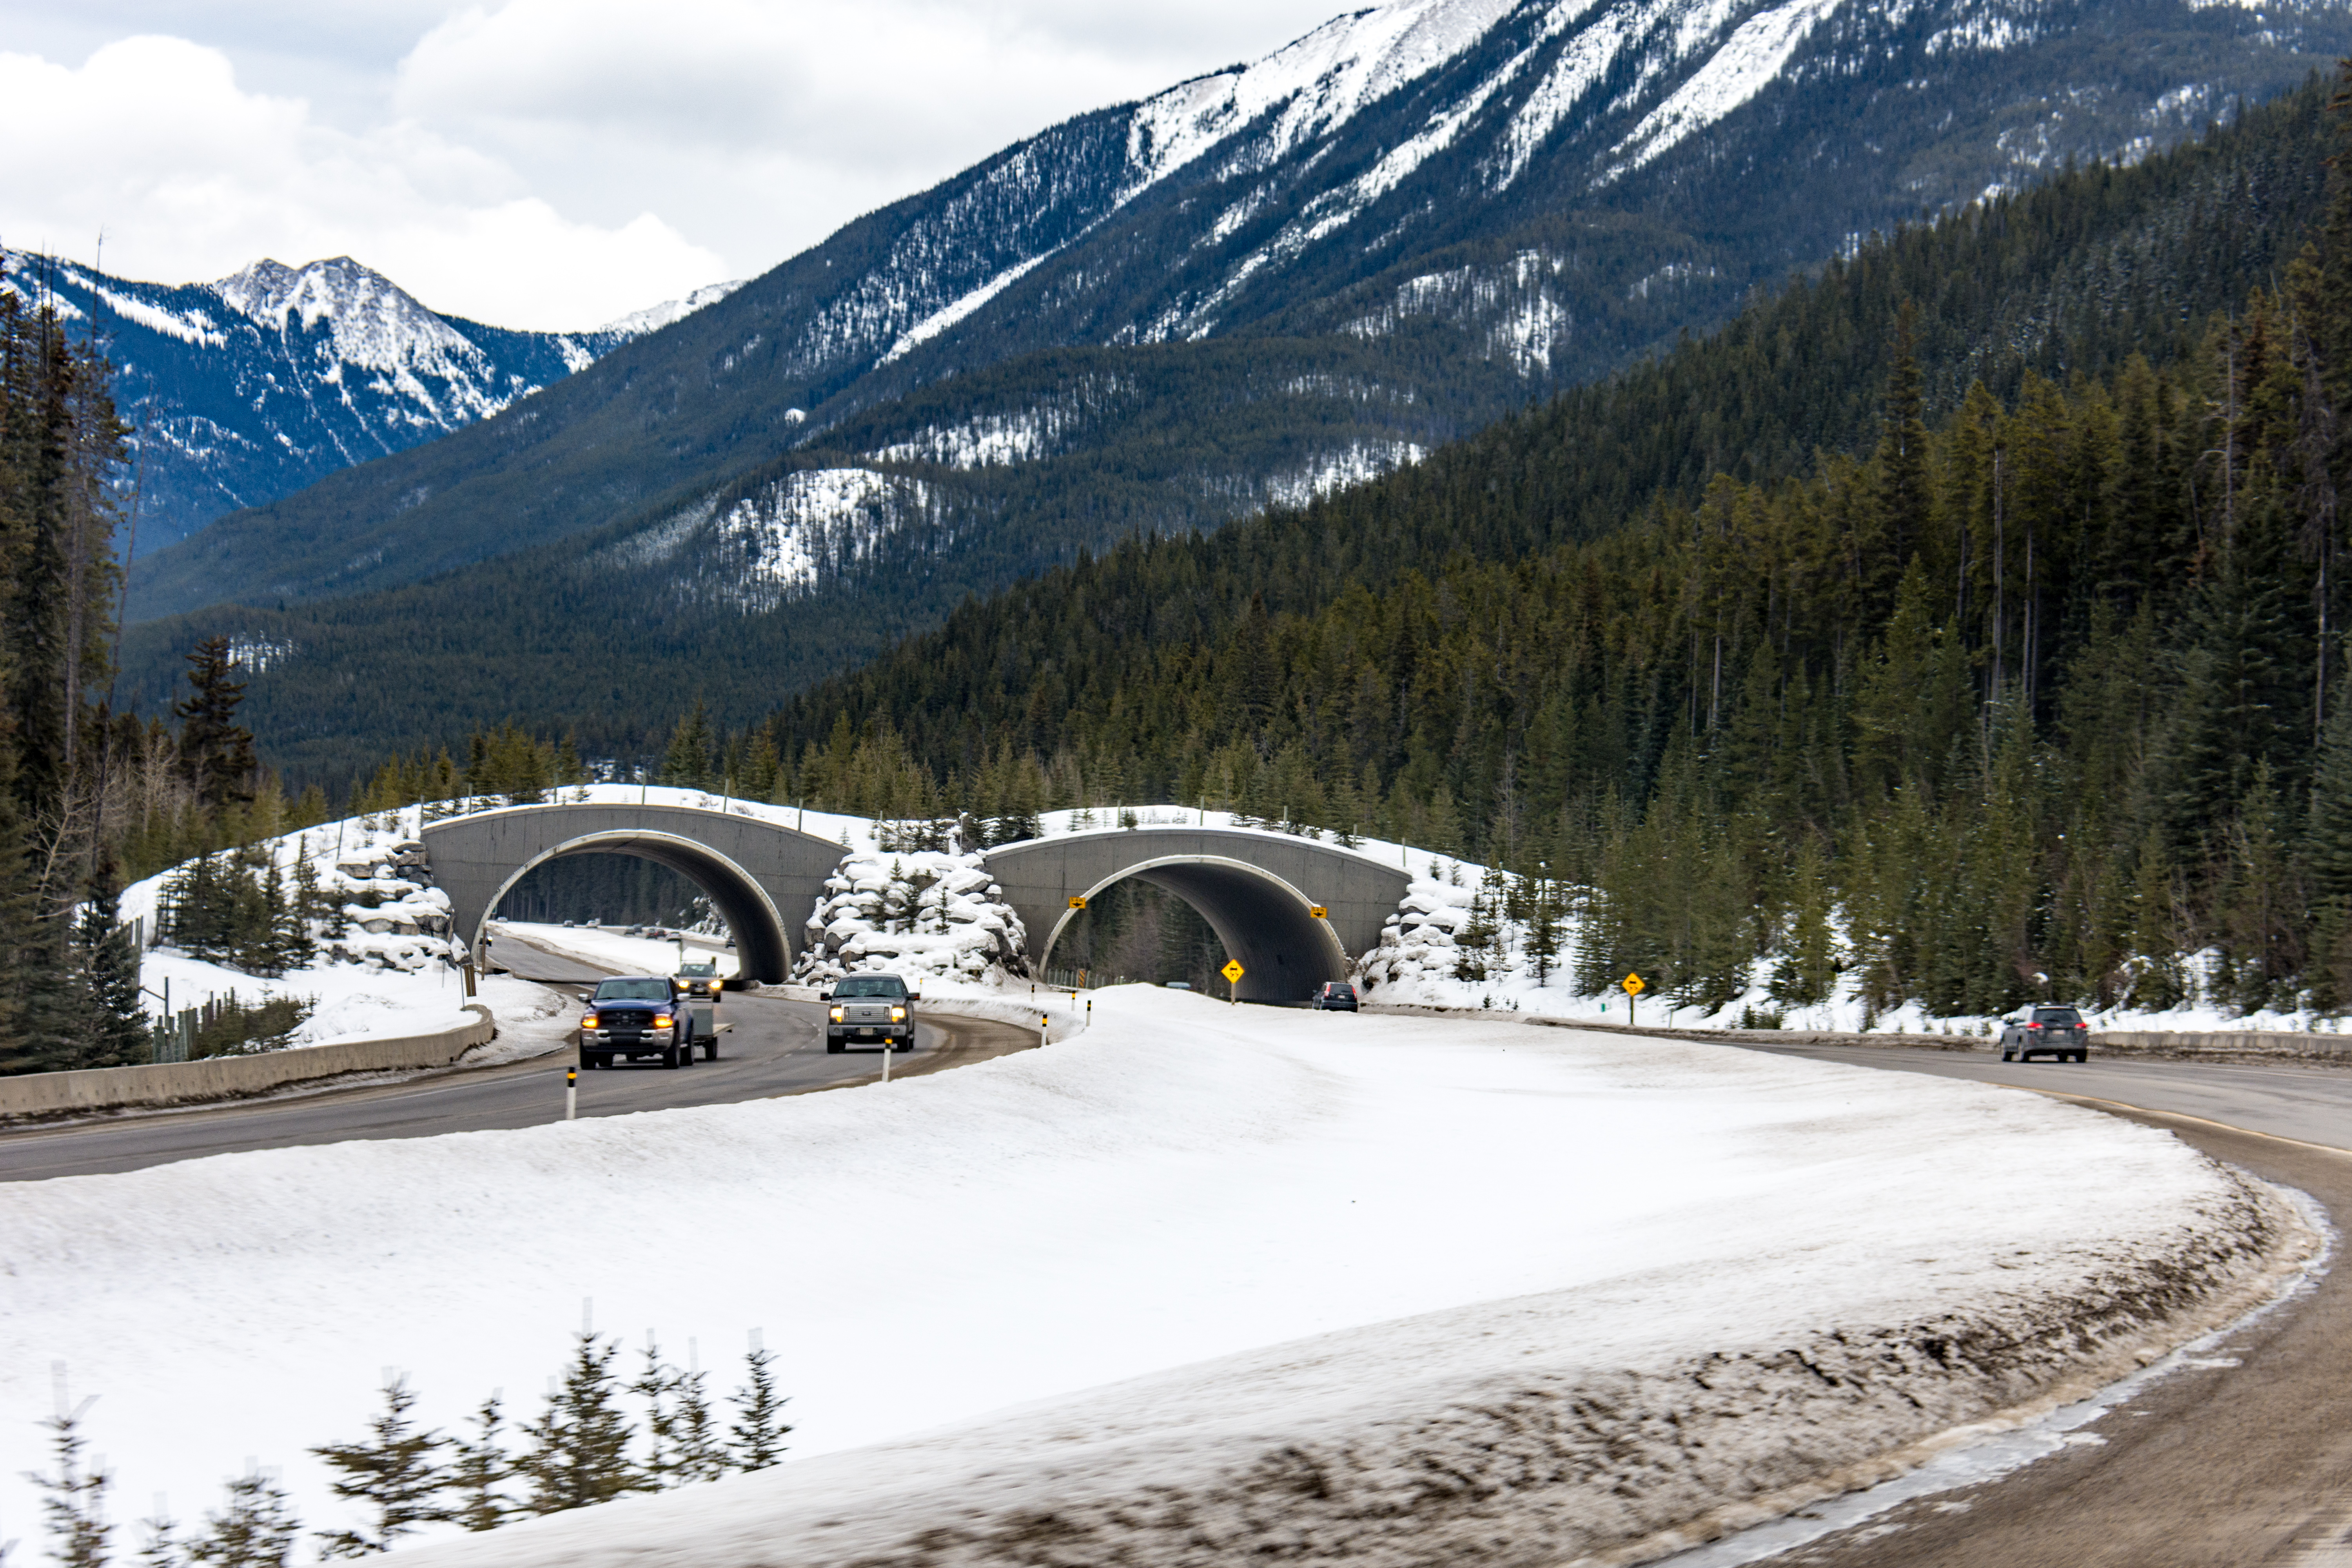
\includegraphics[width=0.46\linewidth]{banff-crossing.jpg}
\end{center}
{\small\textbf{A real wildlife crossing.} In Banff National Park, Canada, traffic passes beneath a habitat connection across the highway. The road still occupies habitat. The photo alone cannot establish animal use or population recovery.\par}
{\footnotesize Photograph: m01229, \href{https://commons.wikimedia.org/wiki/File:Animal_crossing_overpass_in_Banff_National_Park_-_Canada_(26271251055).jpg}{Animal crossing overpass in Banff National Park -- Canada}, Wikimedia Commons, \href{https://creativecommons.org/licenses/by-sa/2.0/}{CC BY-SA 2.0}. Reproduced without content changes; scaled for layout.\par}
\subsection*{Four mechanisms}
\begin{enumerate}
\item \textbf{Loss:} development removes feeding and breeding sites. Resource supply and carrying capacity can decrease.
\item \textbf{Isolation:} individuals may struggle to find mates or recolonize a patch. Reduced gene flow can compound the problem over generations.
\item \textbf{Edge effects:} temperature, moisture, predators, and human disturbance may differ near habitat boundaries.
\item \textbf{Connectivity:} a suitable corridor can support migration, mating, and movement toward newly suitable habitat as conditions change.
\end{enumerate}
Protecting large areas and restoring degraded habitat support resource availability. Corridors support movement. A crossing does not eliminate every road hazard or replace all habitat removed by development.
\subsection*{CHIPPO threats can interact}
A road can remove habitat, introduce pollutants, and provide a route for introduced species. Climate change may further reduce the suitability of isolated patches. Identify the interacting mechanisms instead of assigning one label and stopping.
\memorycheck{A corridor increases immigration into one patch. Does that prove the total regional population grew?}
\classsource{Biodiversity Worksheet; Threats to Biodiversity Notes; Ecology 2 framework, page 1.}


\pagechapter{2B\quad Writing a scientific argument}{cer}
\idea{A strong CER answer links a claim to relevant evidence using a biological mechanism.}
\begin{description}[leftmargin=0pt,labelindent=0pt,itemsep=1pt,topsep=2pt]
\item[Claim] Directly answer the question with a specific, defensible conclusion.
\item[Evidence] Use observations or measurements, including units and meaningful comparisons. Do not invent data.
\item[Reasoning] Explain why the evidence supports the claim using a scientific principle. Address an alternative explanation when relevant.
\end{description}
\subsection*{Worked example with invented practice data}
\begin{wrapfigure}{r}{0.28\linewidth}
\vspace{-14pt}
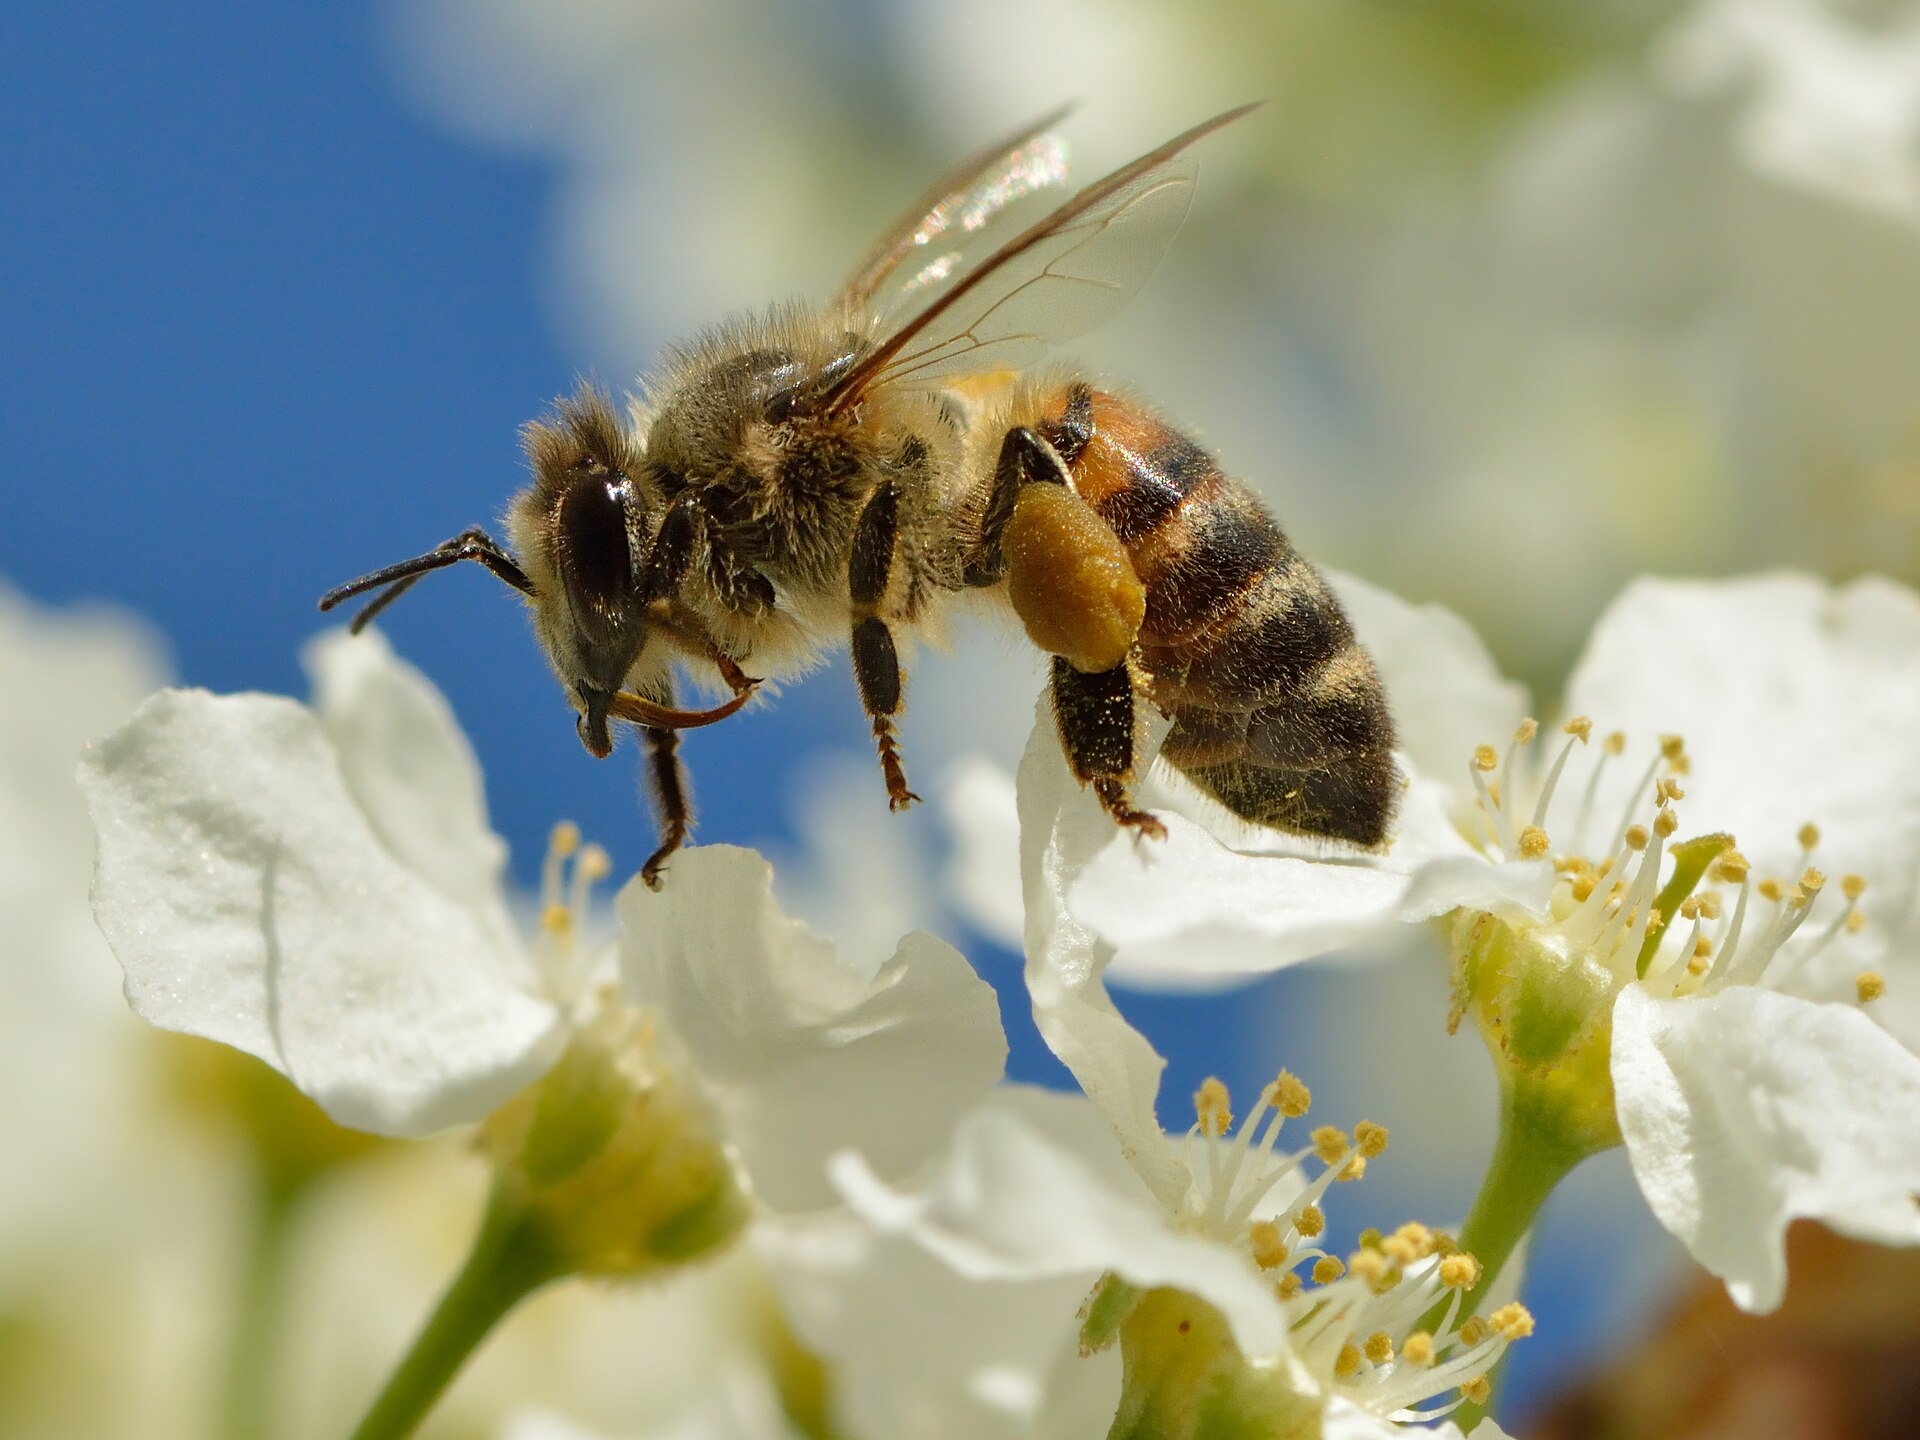
\includegraphics[width=\linewidth]{honeybee-blossom.jpg}
{\footnotesize A honey bee on bird cherry blossom, with pollen on its body and in the basket on its hind leg. \mbox{Ivar Leidus}, \href{https://commons.wikimedia.org/wiki/File:Apis_mellifera_-_Prunus_padus_-_Keila.jpg}{Wikimedia Commons}, \href{https://creativecommons.org/licenses/by-sa/4.0/}{CC BY-SA 4.0}.\par}
\vspace{-10pt}
\end{wrapfigure}
\textbf{Question:} Does a flower strip appear to support pollinator visits?

In this hypothetical study, three equal-sized plots with flower strips averaged 24 visits per hour; three similar plots without strips averaged 9. Observations used the same duration and comparable weather.

\textbf{Claim.} The results support the idea that flower strips increase pollinator visitation under the conditions tested.

\textbf{Evidence.} Plots with flower strips averaged 24 visits per hour, compared with 9 without strips, a difference of 15 visits per hour.

\textbf{Reasoning.} Flowers provide nectar and pollen, so additional floral resources can attract pollinators. Greater visitation in the plots with flower strips is consistent with that mechanism. More visits do not by themselves prove an increase in pollinator population size or species diversity.

\textbf{Limitation.} Unmeasured plot differences could contribute to the result. Random assignment, repeated sampling, and measuring additional variables would strengthen the inference.
\subsection*{Make each sentence do a job}
\begin{itemize}
\item Name the organism, variable, or resource instead of using a vague pronoun.
\item Replace ``restores balance'' with the mechanism: ``increases prey mortality, reducing grazing pressure.''
\item Use \textbf{because} to connect evidence and mechanism; a repeated claim is not reasoning.
\item Match the strength of the conclusion to the evidence. A correlation can motivate a hypothesis without proving causation.
\end{itemize}
\textbf{Teacher writing emphasis.} Section 1C discourages vague words such as ``thing,'' ``normal,'' and ``balance,'' and asks for care with ``adapt'' and ``healthy.'' Prefer precise processes and measurable outcomes.

\textbf{Adaptation versus immediate response.} Evolutionary adaptation concerns inherited traits across generations. An individual sweating or moving into shade is responding to conditions, not evolving during that event.
\memorycheck{Write a three-sentence CER about habitat fragmentation using the mechanism on the previous page. Label hypothetical evidence as hypothetical.}


\pagechapter{2B\quad CER template and rubric}{certemplate}
\idea{Use this page for every CER in class and in this book. Fill in the template, then score yourself with the rubric before you look at any answer key.}
\subsection*{Template}
\par
\begin{tabularx}{\linewidth}{@{}p{0.17\linewidth}Y@{}}\toprule
Part & Write it here\\\midrule
Question & What exactly is being asked? Copy the question.\\[18pt]
Claim & One sentence that answers the question directly. Starters: \textit{The data support the idea that\ldots} \textit{Under the conditions tested,\ldots}\\[18pt]
Evidence & The measurements, with units and a comparison. Starters: \textit{Plots with\ldots averaged\ldots compared with\ldots} \textit{The count fell from\ldots to\ldots over\ldots}\\[26pt]
Reasoning & \textit{because} + the mechanism + the principle. Starters: \textit{This happens because\ldots} \textit{Less\ldots means\ldots, so\ldots} \textit{This matches the principle that\ldots}\\[26pt]
Alternative or limitation & Another explanation, or what the data cannot show. Starters: \textit{The result could also be explained by\ldots} \textit{These data do not show\ldots, so\ldots would strengthen the argument.}\\[18pt]\bottomrule
\end{tabularx}
\par
\subsection*{Rubric}
\par
{\small\begin{tabularx}{\linewidth}{@{}p{0.12\linewidth}Y Y Y@{}}\toprule
Part & 3 Strong & 2 Developing & 1 Weak\\\midrule
Claim & Specific, directly answers the question, matches the strength of the evidence & Answers the question but vague or overstated (``proves'') & Restates the question or does not take a position\\
Evidence & Numbers with units and a comparison; only relevant data & Data mentioned without numbers or without a comparison & No data, or invented data\\
Reasoning & ``Because'' links evidence to a named mechanism and a scientific principle & Mechanism named but not connected to the evidence & Repeats the claim; no mechanism\\
Alternative & Names a plausible alternative or limitation and what would resolve it & Mentions uncertainty without a specific alternative & None\\
Language & Names organisms, variables, and processes; no banned words & One vague word or pronoun & ``It,'' ``thing,'' ``balance,'' ``natural,'' or ``healthy'' carry the argument\\\bottomrule
\end{tabularx}}
\par
\textbf{Scoring.} 13--15 is exam-ready. Below 10, rewrite the reasoning first: most weak CERs fail there. \textbf{Banned words} from the teacher: it, something, thing, normal, natural, balance. \textbf{Use with care:} adapt (evolution across generations, not an individual's response), healthy (say what is measured instead).
\memorycheck{Write a CER for the drought data in practice test A (page \pageref{testa}) using only this template, then score it.}
\pagechapter{2C\quad Vocabulary}{vocabtwoc}
\idea{Population words describe counting, growth, limits, and human demand. Keep the symbols with the terms.}
\begin{vocabtable}
\vt[blue]{\faUsers}{Population} & All the individuals of one species living in a defined area. & The rabbits in one meadow (page \pageref{twoc}).\\
\vt[forest]{\faArrowRight}{Immigration / emigration} & Immigration: individuals moving into a population. Emigration: individuals moving out. & $\Delta N=(B+I)-(D+E)$\\
\vt[blue]{\faChartLine}{Exponential growth} & Growth by a constant percentage, giving a J-shaped curve; bigger populations add more individuals each interval. & Bacteria doubling in fresh broth (page \pageref{curves}).\\
\vt[forest]{\faChartArea}{Logistic growth} & Growth that slows as resources become limiting, giving an S-shaped curve that levels off near carrying capacity. & The idealized model, not an exact trace of real populations.\\
\vt[heat]{\faApple*}{Limiting factor} & Anything that restricts population growth: food, water, space, disease, or weather. & Food supply after a drought.\\
\vt[fur]{\faUserFriends}{Density-dependent / independent} & Dependent: the effect per individual changes with crowding. Independent: the effect is not caused by crowding. & Dependent: competition, disease. Independent: freeze, flood.\\
\vt[orange]{\faBalanceScale}{Carrying capacity ($K$)} & The population size an environment can support over time with its resources and conditions. It can change. & $K$ falls when habitat is lost (page \pageref{changingk}).\\
\vt[soil]{\faShoePrints}{Ecological footprint} & An estimate of the productive land and water needed to supply what a person or population uses and to absorb its wastes. & Compared with biocapacity on page \pageref{humans}.\\
\vt[forest]{\faGlobeAmericas}{Biocapacity} & The ability of ecosystems to regenerate resources and absorb wastes in a year. & Regrowth of forests and crops; absorption of carbon dioxide.\\
\vt[orange]{\faCalendar*}{Earth Overshoot Day} & The estimated date when humanity's demand for the year exceeds what Earth can regenerate that year. & An earlier date means greater demand relative to regeneration (page \pageref{resources}).\\
\vt[blue]{\faHandsHelping}{Environmental justice} & Fair treatment and meaningful participation of all people in environmental decisions, including who bears the burdens and who receives the benefits. & One community drinks the polluted water while many use the factory's products.\\
\end{vocabtable}
\academic{Capacity; decline; exacerbate; exceed; factor; finite; fluctuate; indefinitely; limit; outcome; replenish.}{vocabtwo}
\memorycheck{Write the population equation from memory and label every symbol. Then explain in one sentence why carrying capacity is not a fixed number.}

\pagechapter{2C\quad Population change and limits}{twoc}
\idea{Population size changes through births, deaths, immigration, and emigration. Resources and conditions affect all four processes.}
A \textbf{population} is a group of organisms of the same species in a defined area. Over a stated interval:
\[
\Delta N=(B+I)-(D+E),\qquad N_{\mathrm{new}}=N_{\mathrm{old}}+\Delta N
\]
$B$ = births, $I$ = immigration (moving in), $D$ = deaths, and $E$ = emigration (moving out). Use counts for the same interval and area.

\textbf{Worked example.} A population starts at 200. There are 40 births, 12 immigrants, 25 deaths, and 7 emigrants:
\[
\Delta N=(40+12)-(25+7)=20,\qquad N_{\mathrm{new}}=220.
\]
A flat population graph does not mean births and deaths stopped; it can mean total gains equal total losses.
\subsection*{Limiting factors}
\par
\begin{tabularx}{\linewidth}{@{}p{0.29\linewidth}Y@{}}\toprule
Type & How to recognize it\\\midrule
Density dependent & Its effect per individual tends to change with crowding. Examples include competition for food or nesting space and transmission of some diseases.\\
Density independent & Its impact is not caused by crowding. A severe freeze, fire, or flood can affect sparse and crowded populations, although actual damage depends on context.\\\bottomrule
\end{tabularx}
\par
\subsection*{Carrying capacity is conditional}
\textbf{Carrying capacity} ($K$) is the population size an environment can support over time with its available resources and conditions. It is specific to the organism, place, and conditions, not a permanent universal number.
\begin{itemize}
\item More usable food or habitat can raise $K$; drought, contamination, and habitat destruction can lower it.
\item As a population grows, resources per individual may decline, lowering birth rates or raising death rates. This can act like negative feedback.
\item Delayed responses, seasons, migration, and changing resources can cause populations to fluctuate around a changing $K$.
\item An extreme event can cause immediate mortality, alter $K$, or both. Overshoot can deplete resources and contribute to a later decline.
\end{itemize}
\memorycheck{A pond dries down to half its area. Explain why fish numbers might decline even if fishing has stopped.}

\pagechapter{2C\quad Reading population graphs}{curves}
\idea{A model simplifies reality. Use its shape to explain a mechanism, then state which conditions the model assumes.}
\begin{center}
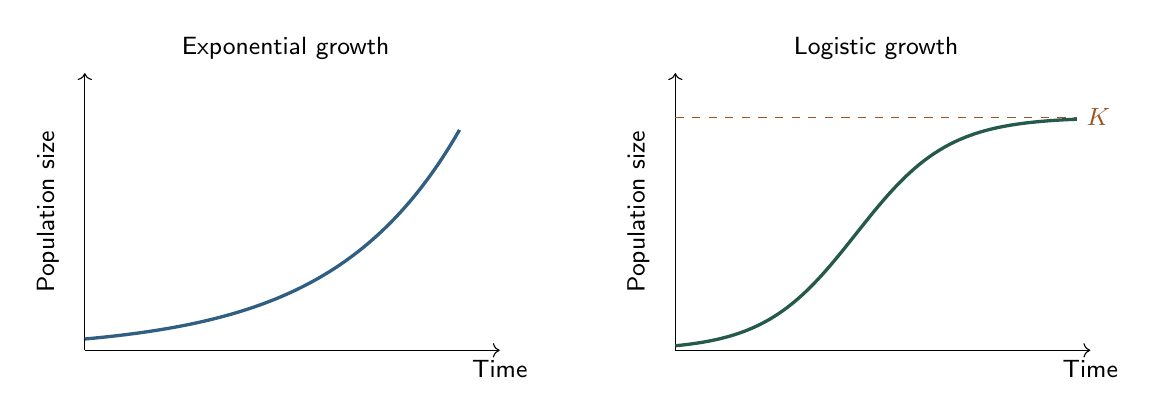
\begin{tikzpicture}[x=0.85cm,y=0.8cm,font=\small\sffamily]
\draw[->] (0,0)--(6.2,0) node[below]{Time};
\draw[->] (0,0)--(0,4.4);
\node[rotate=90] at (-0.55,2.2) {Population size};
\draw[blue,very thick,domain=0:5.6,samples=70] plot (\x,{0.18*exp(0.53*\x)});
\node at (3,4.8) {Exponential growth};
\begin{scope}[xshift=7.5cm]
\draw[->] (0,0)--(6.2,0) node[below]{Time};
\draw[->] (0,0)--(0,4.4);
\node[rotate=90] at (-0.55,2.2) {Population size};
\draw[dashed,orange] (0,3.7)--(6,3.7) node[right]{$K$};
\draw[forest,very thick,domain=0:6,samples=80] plot (\x,{3.7/(1+exp(-1.45*(\x-2.7)))});
\node at (3,4.8) {Logistic growth};
\end{scope}
\end{tikzpicture}\par
\end{center}
\textit{Schematic curves, not observations.} Axes show relative population size and time.

\textbf{Exponential growth} produces a J-shaped curve under sustained positive per-capita growth with resources not yet limiting. A fixed percentage increase means larger populations add more individuals per interval. Growth cannot continue indefinitely in a finite environment.

\textbf{Logistic growth} produces an idealized S-shaped curve. Growth slows as resource limitations increase near $K$. It is useful even though real populations often fluctuate instead of following a perfectly smooth line.
\begin{center}
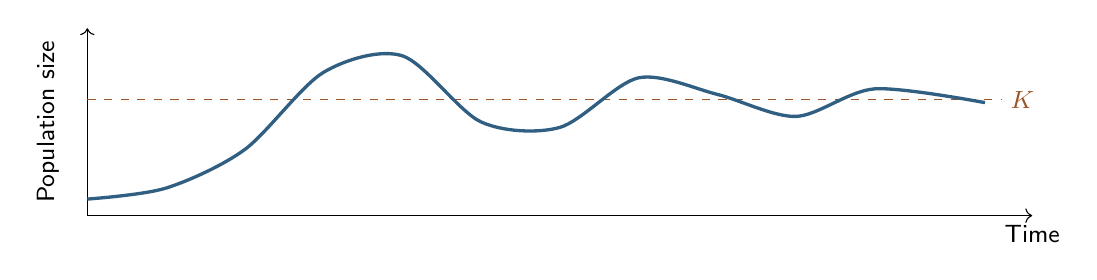
\begin{tikzpicture}[x=1cm,y=0.7cm,font=\small\sffamily]
\draw[->] (0,0)--(12,0) node[below]{Time};
\draw[->] (0,0)--(0,3.4);
\node[rotate=90] at (-0.5,1.7) {Population size};
\draw[dashed,orange] (0,2.1)--(11.6,2.1) node[right]{$K$};
\draw[blue,very thick] plot[smooth] coordinates {(0,0.3)(1,0.5)(2,1.2)(3,2.6)(4,2.9)(5,1.7)(6,1.6)(7,2.5)(8,2.2)(9,1.8)(10,2.3)(11.4,2.05)};
\end{tikzpicture}\par
\end{center}
\textit{Illustrative fluctuation with a reference $K$.} Real $K$ may also change; the horizontal line is an assumption here.
\subsection*{A graph-reading routine}
Read the axes and units; describe where the population rises, falls, or stays similar; compare gains with losses; propose a mechanism; then state what the graph cannot establish. A declining curve alone cannot distinguish increased deaths from increased emigration.
\memorycheck{Near the flat part of a logistic curve, must the birth rate be zero? Explain.}

\pagechapter{2C\quad When carrying capacity changes}{changingk}
\idea{Environmental capacity and actual population size can change at different times. Lower resources do not instantly remove all individuals above a new limit.}
\begin{center}
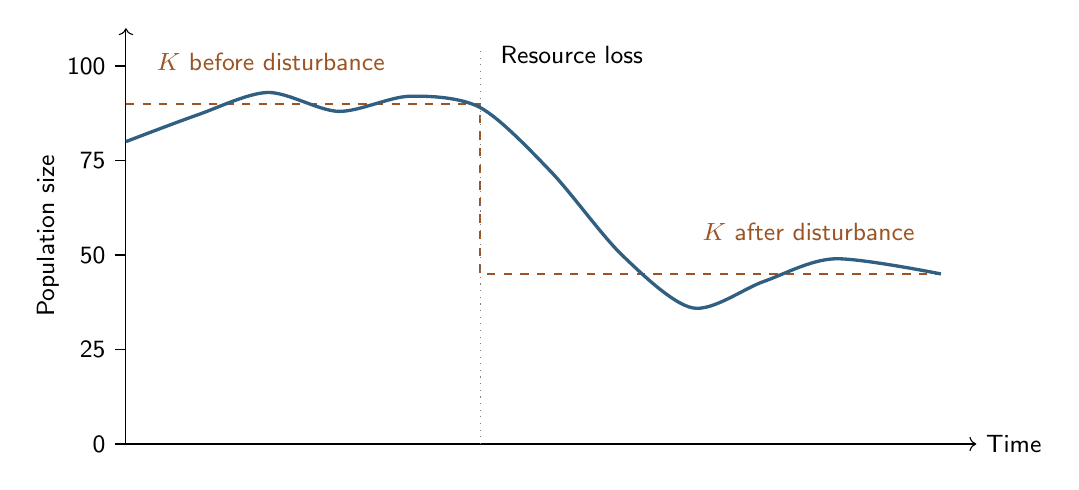
\begin{tikzpicture}[x=0.9cm,y=0.048cm,font=\small\sffamily]
\draw[->] (0,0)--(12,0) node[right]{Time};
\draw[->] (0,0)--(0,110);
\node[rotate=90] at (-1.1,55) {Population size};
\foreach \y in {0,25,50,75,100} {\draw (0,\y)--(-0.15,\y) node[left]{\y};}
\draw[orange,thick,dashed] (0,90)--(5,90)--(5,45)--(11.5,45);
\draw[blue,very thick] plot[smooth] coordinates {(0,80)(1,87)(2,93)(3,88)(4,92)(5,89)(6,72)(7,50)(8,36)(9,43)(10,49)(11.5,45)};
\draw[gray,dotted] (5,0)--(5,105);
\node[anchor=west,text=orange] at (0.3,101) {$K$ before disturbance};
\node[anchor=west,text=orange] at (8,56) {$K$ after disturbance};
\node[anchor=west] at (5.15,103) {Resource loss};
\end{tikzpicture}\par
\end{center}
\textit{Invented illustration.} Orange dashes show $K$; blue shows population size. Values illustrate a pattern, not observations of a particular species.
\subsection*{Interpret the sequence}
Resource loss lowers $K$. The population initially remains above the new capacity, then responds through changes in births, deaths, and movement. Delays and environmental variation can produce later fluctuations.
\begin{center}
\begin{tikzpicture}
\node[pnode] (n) at (0,0) {\tikz{\pic[scale=0.42]{rabbit=fur};\pic[scale=0.42] at (0.85,0.05){rabbit=fur};\pic[scale=0.42] at (1.7,0){rabbit=fur};\pic[scale=0.5] at (0.85,-0.75){grass=leaf};}\\[2pt]More individuals\\share finite resources};
\node[pnode] (r) at (7.8,0) {\pn{leaf}{\faSeedling\,\ico[black!55]{\faDivide}{13pt}\,\ico[fur]{\faPaw}{15pt}}{Less resource\\per individual}};
\node[pnode] (b) at (7.8,-3.2) {\pn{orange}{\faBaby\ico[black!55]{\faArrowDown}{11pt}\quad\ico[black!70]{\faSkullCrossbones}{17pt}\ico[black!55]{\faArrowUp}{11pt}}{Births decrease or\\deaths increase}};
\node[pnode] (g) at (0,-3.2) {\pn{blue}{\faChartLine}{Population growth\\slows or reverses}};
\draw[flow] (n)--node[rel,above]{can mean}(r);
\draw[flow] (r)--node[rel,right]{can cause}(b);
\draw[flow] (b)--node[rel,below]{so}(g);
\draw[flow] (g)--node[rel,left,text width=2cm]{reduces future\\crowding}(n);
\end{tikzpicture}\par
\end{center}
\textbf{Size} is a count. \textbf{Density} is individuals per area or volume. \textbf{Dispersion} is their spacing, such as clustered, uniform, or random. \textbf{Demography} includes age structure and patterns of births and deaths. These measurements answer different questions.
\memorycheck{After a wildfire, distinguish immediate mortality from a reduction in the number of organisms the remaining habitat can sustain.}
\classsource{Population Ecology KJ, slides 2--14; Population Ecology Skeleton Notes; Ecology 2 framework, page 2.}


\pagechapter{2C\quad Human resource use}{humans}
\idea{Human demand depends on population, consumption, and technology. Sustainability also depends on regeneration, waste absorption, and who bears the costs.}
\subsection*{Ecological footprint and overshoot}
An \textbf{ecological footprint} estimates demand on biologically productive land and water, including resource provision and carbon dioxide absorption within the accounting framework. \textbf{Biocapacity} describes ecosystems' capacity to regenerate biological resources and absorb the accounted wastes.

\textbf{Earth Overshoot Day} is the estimated date when humanity's cumulative annual demand exceeds what Earth can regenerate that year. Its calculation compares annual biocapacity with annual ecological footprint. An earlier date indicates greater demand relative to regeneration; a later date indicates less. The date is an estimate, changes with demand and biocapacity, and can be revised as data and methods improve. It does not mean all resources physically run out that day, and it is not a direct biodiversity count.
\source{Global Footprint Network, \href{https://overshoot.footprintnetwork.org/about-earth-overshoot-day/}{About Earth Overshoot Day} and \href{https://footprintnetwork.org/our-work/earth-overshoot-day/}{calculation updates}. No particular year's date is needed here.}
\subsection*{Human carrying capacity is not a fixed head count}
Food systems, water availability, energy use, technology, consumption patterns, and environmental damage change how many people can be supported under particular living conditions. Resource extraction can temporarily support high consumption while degrading future productive capacity. ``Renewable'' does not mean available without limits: a forest can regrow, but harvesting faster than regrowth can deplete it.
\subsection*{Environmental justice}
\textbf{Environmental justice} concerns fair treatment and meaningful participation in environmental decisions. Benefits from resource use and burdens from pollution or scarcity are often distributed unequally. Consider who gets clean water, who lives near pollution, who pays for protection, and whose views influence decisions.

\textbf{Example.} Two communities use goods made by the same factory, but only one experiences contaminated local water. Evaluating resource use requires considering the shared benefits, unequal exposure, and access to decision-making, as well as total consumption.
\begin{center}
\begin{tikzpicture}
\node[pnode] (a) at (0,0) {\pn{blue}{\faUsers}{Population and\\per-person demand}};
\node[pnode] (b) at (5.1,0) {\pn{black!65}{\faIndustry\,\ico[soil]{\faTrash}{16pt}}{Resource use\\and waste}};
\node[pnode] (c) at (10.2,0) {\pn{forest}{\faGlobeAmericas\,\ico[heat]{\faHeart}{16pt}}{Ecosystem capacity\\and human well-being}};
\draw[flow] (a)--node[rel,above]{influence}(b);
\draw[flow] (b)--node[rel,above]{affect}(c);
\end{tikzpicture}\par
\end{center}
\memorycheck{Explain how reducing wasted food could reduce demand without reducing the number of people fed.}

\pagechapter{2C\quad Resource demand and environmental justice}{resources}
\idea{Human carrying capacity depends on how resources are used and shared, not just on the number of people.}
\subsection*{Understand the Overshoot Day comparison}
Earth Overshoot Day compares annual ecological demand with annual biological regeneration. In the accounting framework:
\[
\text{day of year}\approx
\frac{\text{annual biocapacity}}{\text{annual ecological footprint}}
\times\text{days in the year}.
\]
\textbf{Hypothetical example.} If annual demand is twice annual biocapacity, the ratio is $1/2$. In a 365-day year, the corresponding date is around day 183. Reducing demand to $1.5$ times capacity moves the comparison to about day 243. These are illustrations, not actual annual dates.
\subsection*{What continued overshoot means}
The population slides describe using resources accumulated in the past, reducing resources available to other organisms and people in the present, and limiting future options. Examples include drawing down slowly replenished groundwater, removing old forests, and using fossil fuels. These examples explain resource pressure; Overshoot Day does not directly measure every resource stock.

\textbf{Biocapacity} is productive capacity, while \textbf{ecological footprint} measures demand in a specified accounting system. A date change can reflect demand, biocapacity, or revised estimates. It cannot by itself establish a particular number of species lost.
\subsection*{Quality of life and fairness}
A higher quality of life does not always require proportionally more resources. Less food waste, efficient buildings, and effective public services can deliver benefits with less input. Technology can improve efficiency, but environmental damage and rebound in consumption can offset gains.

Environmental justice asks who receives the benefits, who experiences pollution or scarcity, and who participates in decisions. A strategy that lowers total consumption can still distribute costs unfairly. Evaluate the ecological mechanism and the distribution of consequences.
\subsection*{Explain a solution with a causal chain}
Reducing food waste can reduce demand for crops, land, water, and energy while maintaining nutrition. Habitat restoration can improve productive capacity and biodiversity. Neither example guarantees a particular global date shift; the outcome depends on scale and other changes.
\memorycheck{Explain why increasing resource extraction now can support short-term consumption while lowering future carrying capacity.}
\classsource{Population Ecology KJ, slides 17--19; Ecology 2 framework, page 2. Formula: \href{https://overshoot.footprintnetwork.org/about-earth-overshoot-day/}{Global Footprint Network}.}


\pagechapter{Vocabulary for precise explanations}{vocab}
The biological terms are defined in their topic sections. These academic words help you express the relationships the teacher asks about.
\par
\begin{tabularx}{\linewidth}{@{}p{0.32\linewidth}Y@{}}\toprule
Words & Meaning in a biology explanation\\\midrule
Assess; assessment & Evaluate understanding or performance against criteria.\\
Commitment; effective & Sustained effort; successful in achieving an intended result.\\
Condition; criteria & A circumstance affecting a system; standards used to judge a claim or classify something.\\
Stable; constant; range & Stable permits bounded variation; constant is unchanging; range is the span of values.\\
Dynamic; equilibrium & Dynamic means changing or involving ongoing processes. Equilibrium describes opposing processes with no net change; homeostasis generally requires ongoing regulation.\\
Mechanism; model & A process explaining how an effect occurs; a simplified representation used to explain or predict.\\
Reinforce & Strengthen a response or change, as in positive feedback.\\
Affect; effect & Affect is usually a verb meaning influence; effect is usually a noun meaning result.\\
Convert; transfer; store & Change form; move between locations or organisms; retain for later use. Energy is transformed or transferred, not created by organisms.\\
Obtain; release; generate & Acquire; let out; produce. Say organisms generate ATP or heat, not that they create energy from nothing.\\
Cycle; process; interact & Move through repeated transfers; a sequence of events; influence one another.\\
Efficient & Producing a given output with less input or waste; specify which input and output.\\
Complex; context; diverse & Having many interacting parts; relevant circumstances; varied in composition.\\
Collapse; resilient & Severe loss of structure or function; able to retain or recover function after disturbance.\\
Resources & Materials, energy sources, or conditions organisms use to survive and reproduce.\\\bottomrule
\end{tabularx}
\par
\memorycheck{Use ``transfer,'' ``convert,'' and ``release'' in three separate accurate sentences about energy.}

\pagechapter{Vocabulary for ecological change}{vocabtwo}
\par
\begin{tabularx}{\linewidth}{@{}p{0.32\linewidth}Y@{}}\toprule
Words & Meaning in a biology explanation\\\midrule
Consumption; exploitation & Use of resources; use or harvest of organisms or resources. Overexploitation exceeds replacement capacity.\\
Destruction; disruption & Removal or severe damage; interference with a process or relationship.\\
Impact; threat & An effect; a potential cause of harm. State the affected organism or process.\\
Migration & Movement between locations, often seasonal; immigration and emigration specify movement relative to a defined population.\\
Prevention; restoration & Avoiding a problem; helping a damaged ecosystem recover structure or functions.\\
Capacity; finite & The amount that can be supported or held; limited in quantity.\\
Decline; fluctuate & Decrease; vary upward and downward over time.\\
Exacerbate; exceed & Make a problem worse; go beyond a limit.\\
Factor; outcome & Something contributing to a result; the result itself.\\
Indefinitely; limit & Without an end; a constraint or boundary. Exponential growth cannot continue indefinitely with finite resources.\\
Replenish & Replace resources as they are used, through regeneration or other supply.\\\bottomrule
\end{tabularx}
\par
\subsection*{Six statements to be able to explain without notes}
\begin{enumerate}
\item An observation and an inference serve different roles in a scientific explanation.
\item Negative feedback opposes a change; homeostasis allows bounded variation.
\item Producers and consumers both use cellular respiration, while producers supply new organic matter to food webs.
\item Energy dissipates as heat; atoms return through matter cycles.
\item Biodiversity can support resilience, but particular species and disturbance conditions matter.
\item Population growth reflects gains, losses, and limits; carrying capacity can change.
\end{enumerate}
\subsection*{Connect rather than memorize}
Complete this sentence with a mechanism: ``A drought can change carrying capacity because \ldots'' Then connect that mechanism to producer growth, herbivore food supply, and biodiversity. This single chain uses ideas from 1C, 2A, and 2C.



\pagechapter{1A\quad Summary sheet}{sumonea}
\idea{One page to reread the night before. Everything here is explained on pages \pageref{onea} to \pageref{classroom}.}
{\setlength{\columnsep}{18pt}\begin{multicols}{2}\raggedcolumns
\sumhead{Observation and inference}
\begin{sumlist}
\item Observation: gathered with senses or instruments. Inference: an interpretation of observations.
\item Quantitative data are numbers; qualitative data are descriptions.
\item Label which is which in every answer. The count is the observation; the cause is the inference.
\end{sumlist}\sumhead{Induction and deduction}
\begin{sumlist}
\item Induction: many observations $\to$ a general explanation (revisable).
\item Deduction: general idea $\to$ a specific, testable prediction.
\item Cycle: observations $\to$ explanation (hypothesis) $\to$ prediction $\to$ test $\to$ new observations.
\item One supporting result does not prove an explanation.
\end{sumlist}
\columnbreak
\sumhead{Class system}
\begin{sumlist}
\item Formative work (homework, practice tests, CFAs) gives feedback and does not directly change the grade.
\item Checkups 15\%, quality assignments 20\%, quizzes and exams 45\%, final 20\%.
\item Exam retake below 80\% needs completed homework and a retake ticket.
\item Use feedback to find the specific gap, practice that skill, reassess.
\end{sumlist}\sumhead{Say it right}
\begin{sumlist}
\item ``The data suggest'' or ``support,'' not ``prove.''
\item Name the confounding factor: moisture, food, sampling area.
\end{sumlist}
\sumhead{Diagrams to redraw from memory}
\begin{sumlist}
\item The reasoning cycle with four boxes and four labeled arrows (page \pageref{classroom}).
\end{sumlist}
\sumhead{Traps}
\begin{sumlist}
\item An inference is not a guess; a good inference is based on evidence.
\item A hypothesis is the explanation; the prediction is the expected result.
\item Deduction is only as reliable as the general idea behind it.
\end{sumlist}
\end{multicols}}

\pagechapter{1B\quad Summary sheet}{sumoneb}
\idea{Life, metabolism, and homeostasis on one page. Details on pages \pageref{oneb} to \pageref{feedback}.}
{\setlength{\columnsep}{18pt}\begin{multicols}{2}\raggedcolumns
\sumhead{Eight characteristics of life}
\begin{sumlist}
\item Made of cells; reproduction (life cycle or lineage); genetic information (DNA); growth and development; use of matter and energy; response to stimuli; homeostasis; evolution of populations.
\item Judge on the whole list. Fire: no cells, no DNA. Dormant seed: living cells. Sterile mule: alive. Virus: no cells, needs a host, usually classified nonliving.
\end{sumlist}\sumhead{Metabolism}
\begin{sumlist}
\item All chemical reactions that build up or break down molecules.
\item Build: photosynthesis, protein synthesis. Break down: cellular respiration, digestion.
\item Respiration transfers energy from sugar to ATP and releases heat (the warm classroom).
\end{sumlist}
\columnbreak
\sumhead{Homeostasis and feedback}
\begin{sumlist}
\item Keeps a condition within a working range; stable is not constant.
\item Negative feedback opposes the change: hot $\to$ sweat $\to$ cooler $\to$ less sweat; cold $\to$ shiver $\to$ warmer $\to$ less shivering.
\item Positive feedback amplifies the change until an endpoint: childbirth contractions.
\item ``Negative'' and ``positive'' describe direction, not good or bad.
\end{sumlist}\sumhead{Investigations}
\begin{sumlist}
\item Control: comparison condition without the treatment.
\item Constant: factor kept the same in every condition.
\item Hypothesis: testable explanation. Prediction: expected result if the hypothesis holds.
\end{sumlist}
\sumhead{Diagrams to redraw from memory}
\begin{sumlist}
\item Both temperature loops with the return arrow (page \pageref{feedback}).
\item A four-box cycle for one condition you choose (page \pageref{oneb}).
\end{sumlist}
\sumhead{Traps}
\begin{sumlist}
\item Homeostasis does not mean matching the outside environment.
\item Reproduction applies to the lineage, not to every individual.
\item A chain that never returns to the original condition is not a feedback loop.
\end{sumlist}
\end{multicols}}

\pagechapter{1C\quad Summary sheet}{sumonec}
\idea{Energy and matter on one page. Details on pages \pageref{onec} to \pageref{pyramids}.}
{\setlength{\columnsep}{18pt}\begin{multicols}{2}\raggedcolumns
\sumhead{Parts and roles}
\begin{sumlist}
\item Ecosystem = organisms + nonliving environment + interactions. Biotic vs abiotic. Habitat (where) vs niche (role).
\item Producer builds organic molecules from CO$_2$; consumers eat; decomposers (fungi, bacteria) return nutrients.
\item Trophic level = feeding position; one organism can hold more than one.
\end{sumlist}\sumhead{Two equations}
\begin{sumlist}
\item Photosynthesis: $6\mathrm{CO_2}+6\mathrm{H_2O}+\text{light}\to\mathrm{C_6H_{12}O_6}+6\mathrm{O_2}$
\item Respiration: $\mathrm{C_6H_{12}O_6}+6\mathrm{O_2}\to6\mathrm{CO_2}+6\mathrm{H_2O}+$ energy (ATP) $+$ heat
\item Plants do both. Decomposers respire too.
\end{sumlist}\sumhead{Energy flows, matter cycles}
\begin{sumlist}
\item Energy: sun $\to$ producer $\to$ consumers $\to$ decomposers, leaving as heat at every step. Never recycled, never created.
\item Matter: atoms move in loops; CO$_2$ $\to$ sugar $\to$ tissue $\to$ CO$_2$ and minerals $\to$ producers again.
\end{sumlist}
\columnbreak
\sumhead{Numbers}
\begin{sumlist}
\item 10\% rule: $E_{\text{next}}=E_{\text{current}}\times0.10$. Two steps: $\times0.01$.
\item Lab heat: $Q\,(\mathrm{Cal})=V\,(\mathrm{L})\times\Delta T\,(^\circ\mathrm{C})$; 0.50 L warmed 4.0 $^\circ$C $=2.0$ Cal.
\item Pyramids of energy are upright; biomass and numbers can be inverted.
\end{sumlist}\sumhead{Top predators at risk}
\begin{sumlist}
\item Little energy reaches the top, so few individuals over large areas.
\item Dependent on every level below; pollutants concentrate upward.
\end{sumlist}\sumhead{Say it right}
\begin{sumlist}
\item Organisms obtain, store, transfer, convert, or release energy. Never ``create'' or ``use up.''
\item Banned: it, something, thing, normal, natural, balance. Careful: adapt, healthy.
\end{sumlist}
\sumhead{Diagrams to redraw from memory}
\begin{sumlist}
\item Food web with feeding arrows from food to eater (page \pageref{web}).
\item Sun, plant, rabbit, decomposers with food, heat, and gas arrows (page \pageref{gases}).
\item Energy pyramid with numbers (page \pageref{pyramids}).
\end{sumlist}
\sumhead{Traps}
\begin{sumlist}
\item Fertilizer supplies minerals, not energy; carbon in plants comes from CO$_2$.
\item Removing frogs does not immediately remove hawks: alternative prey.
\item Chemosynthesis uses chemical energy; lack of oxygen is not its definition.
\end{sumlist}
\end{multicols}}

\pagechapter{2A\quad Summary sheet}{sumtwoa}
\idea{Biodiversity on one page. Details on pages \pageref{twoa} and \pageref{diversity}.}
{\setlength{\columnsep}{18pt}\begin{multicols}{2}\raggedcolumns
\sumhead{Three levels}
\begin{sumlist}
\item Genetic: alleles within a species (coat colors).
\item Species: number of species (richness) and evenness of individuals among them.
\item Ecosystem: variety of ecosystems across a region (forest, wetland, grassland).
\end{sumlist}\sumhead{Resilience}
\begin{sumlist}
\item Ability to keep or recover functions after disturbance.
\item Mechanism: species respond differently, so a function (pollination) continues when one species declines; more links give alternative food.
\item Diversity helps; it does not guarantee survival.
\end{sumlist}
\columnbreak
\sumhead{Ecosystem services}
\begin{sumlist}
\item Provisioning: food, timber, water, medicine.
\item Regulating: water purification, flood control, pollination, climate.
\item Supporting: nutrient cycling, soil formation, photosynthesis.
\item Cultural: recreation, scenery, spiritual value.
\item Always name the category and the process.
\end{sumlist}\sumhead{Species roles}
\begin{sumlist}
\item Keystone: large effect relative to abundance (some predators).
\item Foundation: builds the habitat others use (reef corals).
\item Pollination: pollen transfer enabling fertilization and seeds.
\end{sumlist}
\sumhead{Diagrams to redraw from memory}
\begin{sumlist}
\item Three panels: alleles, species, ecosystems (page \pageref{diversity}).
\item Coral $\to$ reef habitat $\to$ fish community chain.
\end{sumlist}
\sumhead{Traps}
\begin{sumlist}
\item Many individuals of one species is not high species diversity.
\item Not every predator is a keystone species.
\item A photo shows habitat use, not population recovery.
\end{sumlist}
\end{multicols}}

\pagechapter{2B\quad Summary sheet}{sumtwob}
\idea{Threats and conservation on one page. Details on pages \pageref{twob} to \pageref{cer}.}
{\setlength{\columnsep}{18pt}\begin{multicols}{2}\raggedcolumns
\sumhead{CHIPPO, each with a response}
\begin{sumlist}
\item Climate change: habitats shift; cut emissions, protect movement routes.
\item Habitat loss: farming, building, roads, logging, mining; protect and restore.
\item Invasive species: introduced and harmful; prevent and manage.
\item Pollution: chemicals, nutrients, plastics; reduce at the source.
\item Population with consumption; reduce waste and demand.
\item Overexploitation: harvest faster than replacement; sustainable limits.
\end{sumlist}\sumhead{Loss versus fragmentation}
\begin{sumlist}
\item Loss reduces the amount; fragmentation divides into patches.
\item Fragmentation: smaller populations, less movement and gene flow, edge effects, no recolonization.
\item Corridor: restores movement, not the lost habitat.
\end{sumlist}
\columnbreak
\sumhead{Status words}
\begin{sumlist}
\item Endangered: high risk of extinction. Extinct: none remain.
\item Introduced is not the same as invasive: harm defines invasive.
\item Overconsumption: per-person use matters, not just population.
\end{sumlist}\sumhead{CER}
\begin{sumlist}
\item Claim answers the question. Evidence: numbers, units, comparison. Reasoning: ``because'' + mechanism + principle.
\item Address an alternative and a limitation; match the claim to the evidence.
\item Template and rubric on page \pageref{certemplate}.
\end{sumlist}
\sumhead{Diagrams to redraw from memory}
\begin{sumlist}
\item Three fragmentation panels: continuous, road, corridor (page \pageref{twob}).
\end{sumlist}
\sumhead{Traps}
\begin{sumlist}
\item One threat rarely acts alone; name the interacting mechanisms.
\item A corridor increasing movement does not prove regional growth.
\item ``Restores balance'' is not reasoning.
\end{sumlist}
\end{multicols}}

\pagechapter{2C\quad Summary sheet}{sumtwoc}
\idea{Populations and resources on one page. Details on pages \pageref{twoc} to \pageref{resources}.}
{\setlength{\columnsep}{18pt}\begin{multicols}{2}\raggedcolumns
\sumhead{Counting change}
\begin{sumlist}
\item $\Delta N=(B+I)-(D+E)$; $N_{\text{new}}=N_{\text{old}}+\Delta N$.
\item Flat graph: gains equal losses, not zero births.
\item Size (count), density (per area), dispersion (spacing), demography (ages, births, deaths).
\end{sumlist}\sumhead{Growth models}
\begin{sumlist}
\item Exponential, J-shaped: constant percentage growth, resources not limiting.
\item Logistic, S-shaped: growth slows near $K$ as resources per individual fall.
\item Real populations fluctuate: delays, overshoot, seasons, predator--prey cycles.
\end{sumlist}\sumhead{Limiting factors}
\begin{sumlist}
\item Density-dependent: competition, predation, disease, waste.
\item Density-independent: drought, freeze, flood, fire, human disturbance.
\end{sumlist}
\columnbreak
\sumhead{Carrying capacity}
\begin{sumlist}
\item $K$ = what the environment can support over time; specific to place and conditions.
\item Lower $K$: habitat loss, drought, pollution, new competitor. Higher $K$: more food, restoration.
\item Population can sit above a new, lower $K$ before declining.
\end{sumlist}\sumhead{Human demand}
\begin{sumlist}
\item Footprint (demand) versus biocapacity (regeneration).
\item Overshoot Day $\approx$ biocapacity $\div$ footprint $\times$ 365. Demand twice capacity $\to$ about day 183.
\item Earlier date = more demand relative to regeneration; not a species count.
\item Environmental justice: who benefits, who bears burdens, who decides.
\end{sumlist}
\sumhead{Diagrams to redraw from memory}
\begin{sumlist}
\item J and S curves with labeled axes and $K$ (page \pageref{curves}).
\item Population above a lowered $K$ with the delayed decline (page \pageref{changingk}).
\item The crowding loop with four boxes (page \pageref{changingk}).
\end{sumlist}
\sumhead{Traps}
\begin{sumlist}
\item $K$ is not a fixed universal number.
\item A declining curve cannot separate deaths from emigration.
\item Overshoot Day does not mean resources run out that day.
\end{sumlist}
\end{multicols}}
\pagechapter{Teacher study questions\quad Model answers 1A and 1B}{sqone}
\idea{These are the study questions from the teacher's unit guide, answered in the style the class expects: name the concept, give the mechanism, apply it to an example. None of the answers use ``it,'' ``thing,'' ``normal,'' ``natural,'' or ``balance.''}
Cover each answer, write your own, then compare. Page numbers point to the section with the explanation and diagram.
\subsection*{1A\quad Deliberate practice}
\sq{What are the policies for Biology class?}
\ans{According to the supplied class slides, grades come from checkups (15\%, lowest two per semester dropped, no retakes except for an excused absence), quality assignments (20\%), quizzes and exams (45\%; the unit exam can replace a quiz score, and an exam below 80\% can be retaken after completing homework and a retake ticket), and the final exam (20\%). Homework, practice tests, and CFAs are formative: they give feedback without directly changing the grade. Expect 15--30 minutes of focused homework nightly, and ask the teacher or attend tutorial after more than an hour of struggle. Later announcements from the teacher replace these notes (page \pageref{classroom}).}
\sq{How will students know what they need to learn and how they can demonstrate their understanding in Biology?}
\ans{The KUDOS overview and the unit guide state each learning target with its vocabulary and study questions, so students know the expected knowledge in advance. Classwork, homework, skeleton notes, and reviews build that knowledge. Students demonstrate understanding on checkups, quality assignments, quizzes, the unit exam, and the final. Formative practice shows a gap before the graded work, so a student can fix the gap first (page \pageref{onea}).}
\sq{How are observation and inference related to science?}
\ans{An observation is information gathered with the senses or instruments; an inference is an interpretation of observations using prior knowledge. Science begins with observations, uses inferences to propose explanations, and then tests those explanations against new observations. Keeping the two separate matters because an inference can be wrong even when the observation is accurate: ``18 snails in the shaded plot'' is an observation, while ``shade helps snails survive'' is an inference that other factors, such as moisture, could also explain (page \pageref{onea}).}
\sq{What is the difference between induction and deduction? How does this relate to science?}
\ans{Induction reasons from many specific observations to a general explanation: repeated observations of slow growth in shade suggest that light limits growth. Deduction reasons from a general idea to a specific, testable prediction: if light limits growth, then similar seedlings given more light should grow taller. Science uses both in a cycle. Induction produces hypotheses, deduction produces predictions, and measurements test the predictions. Inductive conclusions stay open to revision; a deduction is only as reliable as the general idea and the premises behind the prediction (page \pageref{classroom}).}
\Needspace{10\baselineskip}\subsection*{1B\quad Life, metabolism, and homeostasis}
\sq{What are the criteria to determine if something is alive?}
\ans{The class checklist has eight characteristics: made of cells, reproduction through a life cycle or lineage, genetic information (DNA), growth and development, use of matter and energy (metabolism), response to stimuli, homeostasis, and evolution of populations across generations. An object must be judged on the whole list, not one sign. Fire uses fuel and grows but has no cells or DNA, so fire is not alive. A dormant seed shows little activity but contains living cells and can resume growth. A virus has genetic information and evolves, but has no cells and cannot reproduce without a host cell's machinery, so viruses are usually classified as nonliving (pages \pageref{lifecheck} and \pageref{cells}).}
\sq{Describe and give examples of metabolism.}
\ans{Metabolism is the complete set of chemical reactions in an organism that build molecules up or break molecules down. Building reactions include photosynthesis, in which producers use light energy to make sugar from carbon dioxide and water, and protein synthesis, in which cells join amino acids into proteins. Breaking-down reactions include cellular respiration, in which cells break sugar down with oxygen and transfer the energy to ATP, releasing carbon dioxide, water, and heat, and digestion, which breaks food into molecules small enough to absorb. The class example of a room warming when people enter shows respiration releasing heat (page \pageref{oneb}).}
\sq{How do feedback mechanisms help to maintain homeostasis?}
\ans{Homeostasis keeps an internal condition, such as body temperature, within a working range. A feedback mechanism detects a change in that condition and triggers a response that then affects the same condition. In negative feedback the response opposes the change: when body temperature rises, sweating increases and evaporation removes heat, so temperature falls toward the range and sweating decreases; when temperature falls, shivering releases heat from muscle metabolism and temperature rises. Because the corrective response weakens as the condition returns to its range, the condition stays within limits instead of drifting. Positive feedback, as in childbirth contractions, strengthens a change until an endpoint ends the loop, so positive feedback is not how set ranges are maintained (page \pageref{feedback}).}

\pagechapter{Teacher study questions\quad Model answers 1C}{sqonec}
\idea{The teacher's tip for this target: do not write ``it,'' ``something,'' ``thing,'' ``normal,'' ``natural,'' or ``balance,'' and be careful with ``adapt'' and ``healthy.'' Name the organism, the substance, and the process every time.}
\sq{Describe the movement of energy, oxygen, carbon dioxide, and heat through the organisms in a food web and their environment.}
\ans{Energy enters as sunlight, which producers store in sugar through photosynthesis. Feeding transfers that chemical energy from producers to consumers and from consumers to predators; dead material and waste carry energy to decomposers. In every organism, cellular respiration transfers energy from sugar to ATP and releases heat to the surroundings, so energy moves in one direction and leaves the food web as heat. Oxygen is released into air or water by photosynthesis and taken in by producers, consumers, and aerobic decomposers for respiration. Carbon dioxide moves the opposite way: producers take carbon dioxide in during photosynthesis, and every organism, including decomposers, releases carbon dioxide during respiration. Heat leaves every living group and does not return to the food web (pages \pageref{web} and \pageref{gases}).}
\sq{How does energy flow relate to homeostasis and metabolism?}
\ans{Organisms obtain energy from light or food, and metabolism, especially cellular respiration, transfers that energy to ATP. ATP powers the work that keeps internal conditions within range: muscle contraction during shivering, transport of ions across membranes, and the synthesis of molecules that repair cells. The heat released by metabolism also raises body temperature. Without a continuous supply of energy from the ecosystem, respiration stops, ATP runs out, and homeostasis fails (page \pageref{roles}).}
\sq{What is an ecosystem?}
\ans{An ecosystem is all the organisms living in an area together with the nonliving environment and the interactions among them. The biotic parts include producers, consumers, decomposers, and biologically produced material such as dead leaves; the abiotic parts include sunlight, temperature, water, minerals, and air. A pond ecosystem includes the fish, frogs, algae, and bacteria plus the water, dissolved oxygen, and light that they depend on (page \pageref{onec}).}
\sq{Explain: ``Energy flows and matter cycles through ecosystems.''}
\ans{Energy moves in one direction. Sunlight is captured by producers, passed along by feeding, transferred to ATP by respiration, and finally released as heat that organisms cannot reuse, so an ecosystem needs a constant input of sunlight. Matter moves in loops. Carbon atoms in carbon dioxide become sugar in a producer, then tissue in a consumer, then carbon dioxide again after respiration or decomposition, and producers take up the same atoms again. Decomposers return minerals to soil and water for producers to reuse. Atoms are rearranged but never used up, while the energy carried by those atoms dissipates (page \pageref{onec}).}
\sq{What roles do organisms play in a food web?}
\ans{Producers, such as grass and algae, build organic molecules from carbon dioxide using light energy. Consumers obtain organic matter by eating: primary consumers (herbivores) eat producers, secondary consumers eat primary consumers, and tertiary consumers eat secondary consumers. Omnivores eat both plants and animals, scavengers eat dead animals, and detritivores such as earthworms ingest small pieces of dead organic matter. Decomposers, mainly fungi and bacteria, break down dead material and waste and return nutrients to the soil or water. An organism can hold more than one position: a hawk eating a rabbit is a secondary consumer, and a hawk eating a frog that ate a grasshopper is a tertiary consumer (page \pageref{roles}).}
\sq{What would be the impact if producers, decomposers, or top predators were removed from an ecosystem?}
\ans{Removing producers cuts off the entry of energy and new organic matter, so herbivores lose food first and the loss spreads to predators; stored food delays the effect only briefly. Removing decomposers lets dead material and waste accumulate, and nutrients stay locked in that material instead of returning to soil and water, so producer growth eventually declines. Removing top predators can allow some prey populations to increase and consume more of their food, changing vegetation and other species; the size and timing of the change depend on alternative prey, competition, and other limiting factors (page \pageref{web}).}
\sq{Give two reasons why top predators are especially at risk.}
\ans{First, ecological pyramids show that only about ten percent of the energy at one level reaches the next, so very little energy is available at the top and top predators exist in small populations that need large hunting areas. A small population loses a large share of its members to any added deaths. Second, top predators depend on every level below them: a loss of producers or prey reduces the energy reaching the top, and habitat loss shrinks the prey base and the hunting area. Some persistent pollutants also become more concentrated at each step up the food chain, which adds a third risk (page \pageref{pyramids}).}

\pagechapter{Teacher study questions\quad Model answers 2A and 2B}{sqtwo}
\subsection*{2A\quad Biodiversity}
\sq{What is biodiversity? List several reasons why biodiversity is important to ecosystems and to humans.}
\ans{Biodiversity is the variety of life at three levels: genetic diversity within a species, species diversity within a community, and ecosystem diversity across a region. For ecosystems, biodiversity supports resilience, because different species respond differently to a disturbance and can keep functions such as pollination, decomposition, and nutrient cycling going; a food web with many links offers alternative food sources when one species declines. For humans, biodiversity supplies food, medicines, timber, and fibers, provides clean water, fertile soil, and crop pollination, holds genetic variation useful for breeding crops and livestock, and has cultural and recreational value (page \pageref{twoa}).}
\sq{What are ecosystem services? List some examples.}
\ans{Ecosystem services are benefits that people receive from ecosystem processes. Provisioning services supply materials: food, timber, fresh water, and medicines. Regulating services control conditions: wetlands purify water and absorb floods, forests store carbon and moderate climate, and insects pollinate crops. Supporting services keep the other services working: nutrient cycling, soil formation, and photosynthesis. Cultural services include recreation, scenic value, and spiritual meaning (page \pageref{twoa}).}
\sq{Why do humans need healthy ecosystems to survive?}
\ans{Every human need traces back to an ecosystem process. Producers release the oxygen we breathe and form the base of every food chain, including farmed crops. Wetlands and forests filter drinking water and reduce floods. Decomposers and soil organisms recycle nutrients that keep soil fertile. Pollinators enable most fruit and many vegetable crops. When an ecosystem is degraded, these services shrink or fail, and replacing them with technology is costly or impossible (page \pageref{twoa}).}
\sq{How does species diversity make ecosystems more resilient?}
\ans{Resilience is the ability of an ecosystem to keep or recover its functions after a disturbance. When several species perform a similar function, such as pollination, and respond differently to a change such as drought, some species keep working while others decline, so the function continues. More species also mean more links in the food web, giving consumers alternative food sources. Diversity raises the chance of recovery but does not guarantee survival: the roles of the species and the severity of the disturbance also matter (page \pageref{diversity}).}
\Needspace{10\baselineskip}\subsection*{2B\quad Human threats and scientific argument}
\sq{Describe each of the major threats to biodiversity.}
\ans{CHIPPO lists six. Climate change shifts temperature and rainfall so that habitats become unsuitable faster than species can move. Habitat loss removes or degrades the places organisms live through farming, building, roads, logging, and mining. Invasive species are introduced organisms that spread and harm native species through competition, predation, or disease. Pollution, including chemicals, excess nutrients, and plastics, damages organisms and habitats. Population growth, combined with per-person consumption, raises demand for land, water, and energy. Overexploitation harvests fish, timber, or wildlife faster than the populations can replace their losses (page \pageref{twob}).}
\sq{Describe the main causes of habitat change or loss.}
\ans{Habitat is lost when land is converted for agriculture, housing, industry, and roads, when forests are logged, when mines and dams reshape land and rivers, and when wetlands are drained. Habitat is degraded, rather than removed, by pollution, by invasive species that change vegetation, and by climate change that alters temperature, rainfall, and sea level. Roads and development also fragment habitat into isolated patches (page \pageref{habitat}).}
\sq{How does habitat fragmentation decrease biodiversity?}
\ans{Fragmentation divides one habitat into smaller, separated patches. Each patch supports a smaller population, which is more likely to die out from chance events. Isolation reduces movement between patches, so individuals struggle to find mates, gene flow falls, and an empty patch is not recolonized. Edges of patches are hotter, drier, and more disturbed than interiors, which harms species that need interior conditions. Species that need large ranges, such as top predators, disappear first (page \pageref{twob}).}
\sq{What can humans do to protect species and ecosystems?}
\ans{Match the action to the threat. Protect and restore habitat, and connect patches with wildlife corridors and crossings. Set sustainable harvest limits and protect breeding populations. Prevent the introduction of invasive species and control established ones. Reduce pollution at its source and cut greenhouse gas emissions. Reduce per-person consumption and waste, and use land and water efficiently. Laws that protect endangered species, along with captive breeding and reintroduction, support species that are already rare (page \pageref{habitat}).}
\sq{How do we practice scientific argumentation using CER?}
\ans{A scientific argument has a claim that answers the question, evidence made of observations or measurements, and reasoning that explains, using a scientific principle, why the evidence supports the claim. In class we write CER statements from lab data, compare arguments with classmates, consider alternative explanations, and revise a claim when new evidence conflicts with the original (page \pageref{cer}).}
\sq{Describe strategies for writing a strong CER statement.}
\ans{State a specific, defensible claim that answers the exact question. Quote quantitative evidence with units and a comparison, such as 24 visits per hour versus 9. Connect evidence to claim with ``because'' and a mechanism, not a repeated claim. Address an alternative explanation and state a limitation. Match the strength of the claim to the evidence: a difference between plots supports an idea but does not prove causation. Avoid vague words such as ``it,'' ``thing,'' and ``balance,'' and name the organism, variable, and process (page \pageref{cer}).}

\pagechapter{Teacher study questions\quad Model answers 2C}{sqtwoc}
\sq{What factors determine the change in a population?}
\ans{Population size changes through four processes: births and immigration add individuals, deaths and emigration remove them, so $\Delta N=(B+I)-(D+E)$ over an interval. Each of the four responds to conditions: food, water, shelter, and space affect births and deaths; predators, disease, and competition raise deaths; weather and disasters can kill many individuals at once; and habitat quality elsewhere drives movement in or out (page \pageref{twoc}).}
\sq{Describe the models (curves) for population growth and what factors might affect this growth.}
\ans{Exponential growth produces a J-shaped curve: the population grows by a constant percentage, so larger populations add more individuals each interval. This pattern appears when a small population enters a habitat with plentiful resources. Logistic growth produces an S-shaped curve: growth slows as the population approaches carrying capacity because resources per individual decline, and the curve levels off near $K$. Factors that affect growth include food and water supply, space and nesting sites, predation, disease, competition, weather, and migration. Real populations fluctuate rather than following either smooth line exactly (page \pageref{curves}).}
\sq{What limiting factors reduce populations?}
\ans{Density-dependent factors act more strongly as crowding increases: competition for food, water, or nesting sites, predation, parasites and disease that spread between neighbors, and accumulation of wastes. Density-independent factors act regardless of crowding: drought, freezes, floods, fires, storms, and human disturbances such as habitat destruction or pollution events (page \pageref{twoc}).}
\sq{Why do populations fluctuate around their carrying capacity?}
\ans{Births and deaths respond to resource changes with a delay. A growing population can overshoot $K$ before food becomes scarce; the shortage then lowers births and raises deaths, so the population falls below $K$; resources recover while the population is small, and growth resumes. Seasons, predator--prey cycles, and changes in the environment also move the population and $K$ itself, so the population size oscillates around a value that is not fixed (page \pageref{curves}).}
\sq{How can the carrying capacity of an organism change?}
\ans{Carrying capacity depends on the resources and conditions of a particular place, so anything that changes those changes $K$. Habitat loss, drought, pollution, and a new competitor or predator lower $K$; more food, restored habitat, and wetter conditions raise it. A disturbance can reduce $K$ while the population is still above the new value, which forces a later decline. For humans, agriculture and technology have raised $K$, while degrading soil, water, and climate can lower future $K$ (page \pageref{changingk}).}
\sq{What extreme changes can destabilize populations and ecosystems?}
\ans{Sudden, large changes overwhelm the responses that normally keep populations within limits. Examples include drought, wildfire, floods, volcanic eruptions, and severe storms; disease outbreaks; the arrival of an invasive species; rapid habitat destruction or pollution events such as oil spills; and fast climate shifts. Density-independent events like these can crash a population regardless of its size, and if they remove producers or keystone species, effects spread through the whole food web (page \pageref{changingk}).}
\sq{What is Earth Overshoot Day and why is it changing over time?}
\ans{Earth Overshoot Day is the estimated date each year when humanity's demand for resources and waste absorption exceeds what Earth's ecosystems can regenerate in that entire year; the calculation divides annual biocapacity by the annual ecological footprint and applies the fraction to the length of the year. Over recent decades the date has moved earlier because the footprint grew, driven by population growth, rising per-person consumption, and carbon dioxide emissions, faster than biocapacity. The date can move later when demand falls or efficiency improves, and revisions to the data and methods also shift the date. An earlier date shows growing pressure on resources; the date by itself does not count species lost (page \pageref{humans}).}
\sq{How does environmental justice relate to human resource use?}
\ans{Environmental justice asks who receives the benefits of resource use and who bears the burdens, and whether affected people have a meaningful voice in decisions. Resource extraction, factories, and waste sites are often placed near communities with less political or economic power, so those communities experience polluted water and air while the products go elsewhere. Evaluating a use of resources therefore requires looking at the distribution of costs and benefits, and at access to clean water, safe air, and green space, not only the total amount consumed (page \pageref{resources}).}
\classsource{Study questions from the Ecology Unit Guide (KJ), targets 1A--2C. Answers are original study explanations based on the class materials cited in the linked sections; they are not teacher-issued answers.}
\pagechapter{Review questions\quad Foundations}{practiceone}
These are new practice questions, not copied exam questions. Answer on separate paper before reading the explanations.
\begin{enumerate}
\item \textbf{1A.} A student records 18 snails in a shaded plot and 6 in a sunny plot, then says shade causes more snails to survive. Identify one observation and one inference. Give a possible confounding factor.
\item \textbf{1A.} Write an inductive conclusion and a deductive prediction about the effect of moisture on seedling growth. Explain the difference.
\item \textbf{1B.} Body temperature falls; shivering starts; temperature rises toward its regulated range. Identify the feedback type and explain why the word ``negative'' applies.
\item \textbf{1B.} A student says a plant cannot be alive because it does not walk and cannot reproduce yet. Explain why those facts do not establish the conclusion.
\item \textbf{1C.} Complete the comparison: photosynthesis takes in which gas and releases which gas? Aerobic cellular respiration does the reverse for which gases? Explain whether a plant respires.
\item \textbf{1C.} In the chain grass $\to$ rabbit $\to$ fox, describe the arrow direction. Explain why a fox depends on producers even though it does not eat grass.
\item \textbf{1C.} Producers supply 20,000 energy units per area per year. Assuming 10\% transfer at each step, calculate energy reaching secondary consumers. Explain where energy not transferred to that level can go.
\item \textbf{1C.} A decomposer community declines sharply. Predict one immediate change in dead material and one later effect on producers. State the connecting mechanism.
\item \textbf{1C.} Explain two reasons why a top predator can be vulnerable when habitat is reduced. Connect each reason to its food web or ecological pyramid.
\end{enumerate}
\vfill
\textbf{Self-check.} Could someone follow the cause-and-effect steps in your answer without guessing what ``it'' or ``balance'' means?

\pagechapter{Review questions\quad Ecological change}{practicetwo}
\begin{enumerate}[start=10]
\item \textbf{2A.} Two fields each have five pollinator species. In one, nearly all visits come from one species; in the other, visits are more evenly shared. What feature differs? Why might it matter after disturbance?
\item \textbf{2A.} Give one ecosystem service used by humans and trace the ecological process providing it. Name its service category.
\item \textbf{2B.} Expand CHIPPO. Choose two threats and give a conservation response matched to each mechanism.
\item \textbf{2B.} A road separates a forest into two patches. Explain how a wildlife corridor may help and why habitat protection is still needed.
\item \textbf{2B.} In a hypothetical experiment, 8 of 10 native seedlings survive without an introduced herbivore, compared with 3 of 10 with it. Write a CER about the herbivore's effect. State one limitation.
\item \textbf{2C.} A population starts at 500. In a year there are 90 births, 35 deaths, 20 immigrants, and 45 emigrants. Calculate its new size.
\item \textbf{2C.} Contrast exponential and logistic growth. Explain why a smooth logistic curve is useful even though a real population fluctuates.
\item \textbf{2C.} A drought lowers food supply while a population is above its former carrying capacity. Predict likely consequences and identify what can happen to $K$.
\item \textbf{2C.} Explain what an earlier Earth Overshoot Day indicates. Does that date alone measure the number of species lost? Explain.
\item \textbf{2C.} A factory supplies products nationwide but pollutes one community's water. Explain how environmental justice relates to the situation.
\item \textbf{Across sections.} Construct a five-node knowledge graph beginning with habitat loss and ending with an effect on people. Label every arrow and state one condition that could change your prediction.
\end{enumerate}
\vfill
\textbf{For diagrams.} State whether your arrows show feeding, movement of matter, energy transfer, or cause and effect. Do not silently change arrow meanings.

\pagechapter{Diagram review\quad Applying the class material}{diagrampractice}
These are original review questions based on the supplied class tasks. Draw and explain your answers before checking the answer guide.
\begin{enumerate}
\item \textbf{Cell and virus.} Label a cell membrane, genome, and cellular machinery. Draw a virus beside it and apply the life checklist.
\item \textbf{Feedback.} Draw both branches of temperature regulation. Label condition, response, resulting change, and reduced corrective action.
\item \textbf{Gas and energy.} Draw sunlight, a plant, a rabbit, and aerobic decomposers. Add heat arrows for all living groups and the correct gas arrows to the surroundings.
\item \textbf{Lab.} In invented data, 0.50 L of water warms by $3.0^\circ$C. Estimate heat gained in Calories. Explain the purpose of the no-hand control.
\item \textbf{Biodiversity.} Illustrate variation within one species and variation among species. Explain why the pictures represent different levels.
\item \textbf{Corridor.} Draw a habitat divided by a road and a crossing. Explain effects on movement, gene flow, and habitat amount.
\item \textbf{Changing capacity.} Lower $K$ after a disturbance and draw a delayed population response. Explain the mechanisms.
\item \textbf{CER.} Use actual lab data if available to write a temperature-comparison claim. Separate measured warming from the proposed metabolic explanation.
\item \textbf{Life.} Compare a dormant seed, a fire, and a sterile animal using at least three characteristics.
\item \textbf{Energy.} Explain how digestion, cellular respiration, ATP, and homeostasis are related without saying that matter becomes energy.
\item \textbf{Resources.} If hypothetical demand is 1.25 times annual biocapacity, estimate the corresponding day in a 365-day year. Explain what that comparison does and does not measure.
\item \textbf{Conservation.} A habitat corridor increases movement, but pollution remains. Explain why population recovery is not guaranteed.
\end{enumerate}
\textbf{Diagram checklist.} Label axes and units. Distinguish real data from schematics. Give each arrow a clear meaning and each causal connection a mechanism.


\pagechapter{Answer explanations\quad Foundations}{answersone}
\begin{enumerate}
\item The counts (18 and 6) are observations. The claim about shade causing survival is an inference. Moisture, food, sampling area, or detection could differ. Counts alone do not measure survival rates.
\item Induction: repeated observations suggest that seedlings with adequate moisture grow more. Deduction: if water limits growth, otherwise comparable dry seedlings should grow more when supplied with water. Induction develops a broader idea; deduction predicts a specific outcome from it.
\item Negative feedback: the initial decrease triggers a response that increases temperature, opposing the initial change. The response is not ``negative'' because it is harmful.
\item Locomotion is not a universal criterion for life. A young plant can be cellular, metabolically active, regulated, and developing even before reproductive maturity. Consider the full set of characteristics.
\item Oxygen-producing photosynthesis takes in carbon dioxide and releases oxygen. Aerobic respiration consumes oxygen and releases carbon dioxide. Plants carry out respiration to supply energy for cellular work; photosynthesis does not replace that need.
\item Arrows point from food to consumer, showing transfer of organic matter and chemical energy. Grass supplies the rabbit's food; the fox receives some of that matter and energy by eating the rabbit.
\item $20{,}000(0.10)^2=200$ units per area per year. Energy can be released as metabolic heat or remain in material not passed to the next consumer, including waste and uneaten parts that can support decomposers. Energy is not destroyed.
\item Dead material tends to accumulate. Slower decomposition reduces the return of available nutrients, which can later limit producer growth. Timing depends on existing nutrients and other recycling pathways.
\item Lower energy availability supports fewer individuals at high trophic levels, so additional losses can strongly affect a small population. A predator also needs enough connected habitat and prey production; habitat reduction can shrink the supporting prey base or hunting area. These are tendencies, not guarantees for every species.
\end{enumerate}
\subsection*{Answers to the short memory prompts}
A strong answer names the original change, the mechanism, and the result. For food-web questions, distinguish transfer of atoms from transfer and dissipation of energy. For the graph on page \pageref{web}, rabbits offer the hawk an alternative food source, but their abundance may not be sufficient to replace frogs.

\pagechapter{Answer explanations\quad Ecological change}{answerstwo}
\begin{enumerate}[start=10,itemsep=5pt]
\item Species richness is equal; relative contribution to visits differs. Visit counts alone do not establish the abundance of each species. More evenly distributed activity may reduce dependence on one species. Resilience still depends on how each species responds and whether others can compensate.
\item Example: pollinators transfer pollen, helping crops reproduce and produce fruits or seeds used as food. Pollination is commonly a regulating service; harvested food is provisioning. Explain the process even when a category is not required.
\item Climate change, habitat loss, invasive species, pollution, population, overexploitation. Examples: habitat protection addresses loss; harvest limits address removal faster than reproduction; pollution control reduces exposure.
\item A corridor can permit movement, mating, and recolonization, reducing isolation. It cannot replace all lost feeding or breeding habitat. Design, safety, and the species' behavior affect its usefulness.
\item Claim: the herbivore reduced seedling survival in the trial. Evidence: survival was 3/10 with it versus 8/10 without it. Reasoning: feeding damage can remove tissue needed for photosynthesis or growth. A small sample and unmeasured differences limit inference; introduction alone does not establish invasive status.
\item $\Delta N=90+20-35-45=30$; the new population is $530$.
\item Exponential growth assumes sustained positive per-capita growth without effective resource limitation. Logistic growth incorporates slowing near $K$. Its idealized pattern helps explain density-related limits even when real resources and population sizes vary.
\item Reduced food can lower $K$. Births may decline, deaths or emigration may rise, and overshoot may further deplete resources. Exact timing and magnitude require data.
\item Demand exceeds annual regeneration earlier in the year. This is a resource-accounting indicator, not a measurement of species loss. Resource pressure can harm biodiversity, but biodiversity change needs separate evidence.
\item Benefits are widespread while pollution burdens are concentrated. Fair access to clean water, protection, and meaningful participation by affected residents are environmental-justice concerns.
\item One valid graph: habitat loss $\to$ fewer flowering plants $\to$ less pollinator food $\to$ fewer pollinator visits $\to$ lower crop pollination. Each arrow means ``can cause.'' Other food sources or managed pollination could change the prediction; lower visits do not automatically prove population decline.
\end{enumerate}

\pagechapter{Diagram review\quad Answer guide}{diagramanswers}
\begin{enumerate}[itemsep=5pt]
\item Cells have membranes and metabolic machinery. Viruses contain a genome and coat but require a host cell to assemble new particles. Shared genetic information alone does not establish cellular life.
\item Warming triggers cooling; cooling reduces the need for further cooling. Falling temperature triggers warming; recovery reduces warming responses. Both oppose the initiating change.
\item Light reaches the plant. Organic molecules move along feeding and decomposition pathways. Every living group releases heat. Photosynthesis takes in carbon dioxide and releases oxygen; aerobic respiration reverses these gas directions. Plants need both sets of arrows.
\item $Q=0.50\times3.0=1.5$ Cal, or 1.5 kcal. The control measures changes possible without a hand. Water heating does not capture all energy used by the body.
\item Allelic differences within a species illustrate genetic diversity; different species illustrate species diversity. Individual counts alone establish neither.
\item A usable crossing can support movement, mating, and recolonization without restoring all removed habitat. Movement into a patch may be redistribution rather than regional growth.
\item Actual numbers can initially exceed the new $K$. Reduced births, increased deaths, or emigration can follow. Exact rates require evidence.
\item Cite actual temperatures and elapsed time. Muscle work uses ATP, metabolism supplies usable energy, and heat transfers to the water. Mixing, hand differences, and starting conditions also affect the measured change.
\item The seed has living cells and genetic information despite dormancy. Fire lacks cells and a biological inheritance system. A sterile animal has cellular organization and metabolism despite reproductive inability.
\item Digestion prepares molecules for absorption. Respiration transfers fuel energy to ATP; ATP supports work needed for homeostasis. Atoms are rearranged, and heat is released.
\item $365/1.25=292$: approximately day 292. This illustrates demand relative to regeneration, not the day all resources physically disappear.
\item Pollution can still reduce survival or reproduction. Connectivity addresses one mechanism; recovery also depends on habitat quality and other limiting factors.
\end{enumerate}
\classsource{Original questions and answers based on the class materials cited in the corresponding chapters.}


\pagechapter{Practice test A\quad 15 multiple choice and 1 free response}{testa}
\idea{Same format as the StudyBio practice quiz: 15 multiple-choice items and one free-response item. Allow 35 minutes. Answer on separate paper before opening the key on page \pageref{testakey}.}
\textbf{Use this food web for questions 6 and 7.}
\begin{center}
\begin{tikzpicture}[x=1cm,y=1cm]
\node[scene] (grass) at (0,0) {\tikz{\pic[scale=0.8]{grass=leaf}}\\Grass};
\node[scene] (rabbit) at (3.6,1.1) {\tikz{\pic[scale=0.7]{rabbit=fur}}\\Rabbit};
\node[scene] (hopper) at (3.6,-1.1) {\ico[soil]{\faBug}{20pt}\\Grasshopper};
\node[scene] (frog) at (7.2,-1.1) {\ico[leaf!70!black]{\faFrog}{20pt}\\Frog};
\node[scene] (hawk) at (7.2,1.1) {\ico[black!70]{\faCrow}{22pt}\\Hawk};
\node[scene] (dec) at (10.8,0) {\tikz{\pic[scale=0.8]{mushroom=orange!70!white}}\,\ico[blue]{\faBacteria}{16pt}\\Decomposers};
\draw[feed] (grass)--(rabbit); \draw[feed] (grass)--(hopper); \draw[feed] (rabbit)--(hawk); \draw[feed] (hopper)--(frog); \draw[feed] (frog)--(hawk);
\draw[feed,draw=soil,dashed] (hawk)--(dec);
\end{tikzpicture}
\end{center}
\begin{enumerate}[itemsep=4pt]
\mc{A student writes: ``The stream has fewer mayflies this year, so the water quality has gotten worse.'' Which part of the sentence is an inference?}{fewer mayflies this year}{water quality has gotten worse}{both parts are observations}{neither part is an inference}
\mcl{Which statement is an example of deductive reasoning?}{After measuring 30 shaded plants that grew slowly, a student concludes that shade limits growth.}{If shade limits growth, then shaded seedlings moved into sunlight should grow faster.}{A student notices that the leaves on one plant are yellow.}{A student records the height of every plant in the plot.}
\mcl{Which statement best explains why a virus is usually classified as nonliving?}{A virus cannot evolve.}{A virus contains no genetic material.}{A virus is not made of cells and cannot reproduce without a host cell's machinery.}{A virus is too small to be seen with a light microscope.}
\mcl{During exercise, body temperature rises, sweating increases, temperature falls toward its range, and sweating decreases. This sequence is}{positive feedback, because sweating is helpful.}{negative feedback, because the response opposes the original change.}{positive feedback, because the temperature changed twice.}{not feedback, because the body returned to its range.}
\mcl{A student says a mule cannot be alive because mules are sterile. Which response is correct?}{The student is right; reproduction is required for every individual.}{The student is wrong; the mule shows the other characteristics of life, and reproduction applies to lineages, not every individual.}{The student is right, because sterile animals lack DNA.}{The student is wrong, because movement alone proves life.}
\mcl{In the food web above, the arrow from the grasshopper to the frog means that}{the grasshopper eats the frog.}{matter and chemical energy move from the grasshopper to the frog.}{the frog produces energy for the grasshopper.}{the grasshopper decomposes the frog.}
\mcl{If a disease removed all the frogs from this web, which prediction is best supported?}{Hawks would disappear immediately because they have no other food.}{Grasshoppers might increase at first because one of their predators is gone, while hawks could rely more on rabbits.}{Grass would die because frogs fertilize the soil.}{Decomposers would stop functioning.}
\mcl{Which statement describes the path of energy through an ecosystem?}{Energy cycles from producers to consumers to decomposers and back to producers.}{Energy flows in one direction and leaves the ecosystem as heat.}{Producers create energy from water and minerals.}{Decomposers destroy the energy in dead material.}
\mc{Producers in a field capture 50{,}000 units of energy per year. Using the 10\% rule, about how much energy is available to secondary consumers?}{5{,}000 units}{500 units}{50 units}{45{,}000 units}
\mcl{Which statement about gas exchange is correct?}{Photosynthesis releases carbon dioxide into the air.}{Only animals carry out cellular respiration.}{Plants carry out both photosynthesis and cellular respiration.}{Decomposers do not release carbon dioxide.}
\mcl{Two meadows each contain six flowering plant species. In meadow 1, one species makes up 95\% of the plants. In meadow 2, each species makes up about 17\%. Which statement is best?}{Meadow 1 has higher species diversity because one species dominates.}{Meadow 2 has higher species diversity because individuals are spread more evenly among the species.}{The meadows have equal species diversity because both have six species.}{Species diversity cannot be compared without genetic data.}
\mc{A wetland removes sediment and excess nutrients from water flowing through it. This is which category of ecosystem service?}{provisioning}{regulating}{cultural}{supporting}
\mcl{A new highway divides a forest into two patches. Which is the most direct effect on the deer population?}{Gene flow between the two sides increases.}{Movement between the patches decreases, leaving two smaller, more isolated groups.}{The deer become extinct within a year.}{Each deer receives more food.}
\mcl{A fertilized plot of corn grew 12 cm taller on average than an unfertilized plot. Which reasoning statement is strongest?}{The data show the plants grew more, so the claim is right.}{The fertilized plants grew 12 cm taller on average because the nitrogen in fertilizer is used to build the proteins and chlorophyll needed for growth.}{The plants grew better because fertilizer is natural and healthy for them.}{The fertilized plants were bigger, which restored the balance of the field.}
\mc{A population of 400 deer has 60 births, 25 deaths, 10 immigrants, and 15 emigrants in one year. What is the population at the end of the year?}{430}{370}{460}{510}
\end{enumerate}
\textbf{Free response (16).} A two-year drought reduces grass growth in a meadow. Hypothetical data: grass biomass fell by 60\%, and the rabbit count fell from 120 to 45 over the two years. Write a CER argument about the effect of the drought on the rabbits' carrying capacity, then predict, with a mechanism for each, what happens to (a) the hawks and (b) the decomposers and soil nutrients. Do not use ``it,'' ``thing,'' ``normal,'' ``natural,'' or ``balance.''

\pagechapter{Practice test A\quad Answer key}{testakey}
Each entry gives the answer and the reason every other choice is wrong. If you missed an item, reread the page listed before retrying.
\begin{enumerate}[itemsep=3pt]
\item \textbf{B.} ``Fewer mayflies'' is counted, so A is an observation. C is wrong because the water-quality claim interprets the count. D is wrong because the second part is an inference. (page \pageref{onea})
\item \textbf{B.} A prediction derived from a general idea is deduction. A is induction (specific cases to a general conclusion). C and D are observations, not reasoning. (page \pageref{classroom})
\item \textbf{C.} A is false because viral populations evolve. B is false because viruses carry DNA or RNA. D is true but is not a criterion for life. (page \pageref{cells})
\item \textbf{B.} The sign of feedback describes direction, not helpfulness (A) or the number of changes (C). D is wrong because the return to the range is exactly what negative feedback produces. (page \pageref{feedback})
\item \textbf{B.} Reproduction is a characteristic of life at the level of the life cycle or lineage; an individual that cannot reproduce still has cells, metabolism, and homeostasis. A applies the checklist to the wrong level, C is false (mules have DNA), and D uses a single sign. (page \pageref{lifecheck})
\item \textbf{B.} A food-web arrow points from food to eater and shows the transfer of matter and chemical energy. A reverses the direction, C is wrong because animals do not produce energy, and D confuses feeding with decomposition. (page \pageref{web})
\item \textbf{B.} Hawks have rabbits as an alternative food, so A overstates the effect. C invents a role for frogs, and D ignores that decomposers receive material from every level. (page \pageref{web})
\item \textbf{B.} Energy is not recycled (A), not created (C), and not destroyed (D); each organism releases some as heat. (page \pageref{onec})
\item \textbf{B.} Two transfers at 10\% each: $50{,}000\times0.10\times0.10=500$. A is one transfer, C is three, and D is the energy that did not pass to the next level. (page \pageref{pyramids})
\item \textbf{C.} Photosynthesis releases oxygen, not carbon dioxide (A). Plants, animals, and decomposers all respire (B, D). (page \pageref{gases})
\item \textbf{B.} Species diversity includes evenness as well as richness. A reverses the idea, C ignores evenness, and D confuses the species level with the genetic level. (page \pageref{diversity})
\item \textbf{B.} Water purification regulates a condition. Provisioning supplies materials, cultural covers recreation and meaning, and supporting covers processes such as nutrient cycling. (page \pageref{twoa})
\item \textbf{B.} A road reduces movement, so A is backward. C is too extreme for the evidence, and D is wrong because habitat is lost, not gained. (page \pageref{twob})
\item \textbf{B.} Strong reasoning links the evidence to a mechanism with ``because.'' A repeats the claim, C uses vague words (``natural,'' ``healthy'') instead of a mechanism, and D uses ``balance'' and explains nothing. (page \pageref{cer})
\item \textbf{A.} $400+(60+10)-(25+15)=430$. B subtracts the additions, C ignores the losses, and D adds everything. (page \pageref{twoc})
\end{enumerate}
\subsection*{Free response: a model answer and what earns credit}
\textbf{Claim.} The drought lowered the carrying capacity of the meadow for rabbits. \textbf{Evidence.} Grass biomass fell by 60\%, and the rabbit count fell from 120 to 45, a decline of 75\%, over the same two years. \textbf{Reasoning.} Grass is the rabbits' food, so less grass means less food per rabbit; with less food, fewer rabbits are born and more die, and the number the meadow can support over time falls. The rabbit decline followed the grass decline, which matches this mechanism. A limitation is that disease or emigration could also lower the count, so measuring births, deaths, and movement would strengthen the argument.

\textbf{(a) Hawks.} Rabbits are prey for hawks, so less rabbit biomass means less energy reaching the hawk level; hawk numbers can fall, or hawks may hunt elsewhere or shift to other prey such as frogs. Because hawks sit at the top of the pyramid, a small change in prey can affect a small hawk population strongly. \textbf{(b) Decomposers and soil nutrients.} At first, dead grass and dead rabbits can supply more material to decomposers, but dry conditions slow decomposition, so nutrients return to the soil more slowly and producer regrowth can be limited even after rain returns.

\textbf{Scoring guide.} Claim that names carrying capacity and its direction (2 points). Evidence with both numbers and a comparison (2). Reasoning with the food-supply mechanism and the link to births and deaths (3). One limitation or alternative explanation (1). Predictions for hawks and decomposers, each with a mechanism (2). No banned words (1). Total 11 points.
\classsource{Original practice test in the format of the supplied StudyBio quiz. Questions and answers are study material, not teacher-issued items.}
\pagechapter{Using the supplied practice key carefully}{keynotes}
The supplied file is titled \textit{StudyBio's Practice Ecology Quiz}. It contains 15 multiple-choice questions and one free-response item, with highlighted answers and comments. It is useful practice, but several statements require interpretation or clarification. Keep the original key intact.
\par
\begin{tabularx}{\linewidth}{@{}p{0.13\linewidth}Y@{}}\toprule
Item & What to learn accurately\\\midrule
Q1 & The arrows depict negative feedback. The key also marks the depiction as incorrect, apparently because the labels describe a fixed temperature. That rationale is inferred, not stated. Homeostasis regulates a range; a simplified diagram is not automatically invalid.\\
Q3 & The key selects ``none of the above'' and names the Sun in a note. Sunlight supports most ecosystems, but chemical energy can support chemosynthetic food webs. ``All life'' is too broad.\\
Q5 & Photosynthesis and chemosynthesis can support production of organic molecules. Chemosynthesis uses chemical energy; lack of oxygen is not its defining feature. Cellular respiration is also used by many producers.\\
Q7 & The key rejects the listed combinations. Removing a consumer does not establish immediate changes in every other group. Follow the actual web and distinguish short-term from delayed effects.\\
Q13 & The key selects ``none'' for corridors directly alleviating habitat loss. The likely intended distinction is loss versus fragmentation. Corridors address connectivity and may also restore habitat; the question's wording does not support a universal rejection of corridors.\\
Q14 & The key calls a smooth logistic curve unrealistic. Treat the curve as an idealized model: useful for explaining limits, but not an exact trace of most field populations.\\
Q15 & The key links an earlier Overshoot Day to biodiversity loss. The direct meaning is greater demand relative to annual regeneration. Species loss cannot be established from the date alone.\\\bottomrule
\end{tabularx}
\par
\textbf{Class requirements clarified.} Although the practice key calls some topics class-dependent, the supplied Biodiversity Worksheet explicitly asks for all four ecosystem-service categories and wildlife corridors. Study both.

\textbf{Review strategy.} Attempt the blank quiz first, then compare explanations with the key. When an answer depends on wording, distinguish the intended classroom concept from a statement that is universally true. Ask the teacher about the highlighted ambiguities before using them as exam rules.

\pagechapter{Sources and coverage}{sources}
\subsection*{Class and practice materials}
\begin{itemize}
\item \textit{Ecology Unit Guide (KJ).docx}: learning targets 1A, 1B, 1C, 2A, 2B, and 2C; vocabulary and study-question scope. The guide's listed textbook sections are retained below. The textbook is identified by Shawn's parent as \textit{California Miller \& Levine Biology Student}; the edition and textbook pages have not yet been supplied.
\item \textit{A\_EcologyPracticeQuiz\_KEY.pdf}: StudyBio practice quiz, four pages. Used to identify question styles, CHIPPO wording, extensions, and key ambiguities. This book does not reproduce the quiz.
\item \textit{A\_EcologyPracticeQuiz\_BLANK.pdf}: companion practice paper available in the project for independent attempts.
\end{itemize}
This revision incorporates text from all 26 supplied source files, including eight slide decks, class worksheets, skeleton notes, CER materials, the energy-flow lab, and the Ecology 2 framework. The two copies of the Ecology 2 framework are identical. Class-connection notes identify the relevant sources throughout. Original explanations, diagrams, synthetic data, and new questions supplement the supplied materials; they are not teacher-issued answers. Linked videos and textbook pages were not supplied or reviewed.
\par
\begin{tabularx}{\linewidth}{@{}l l Y@{}}\toprule
Target & Guide textbook reference & Book focus\\\midrule
1A & Not listed & Evidence, reasoning, and deliberate practice\\
1B & 1.3 & Life, metabolism, feedback, and investigation\\
1C & 3.1, 4.1, 4.2, 6.1 & Ecosystems, food webs, energy and matter\\
2A & 6.3 & Biodiversity, resilience, ecosystem services\\
2B & 7.2 & Human threats, conservation, and CER\\
2C & 5.1, 5.2, 5.3 & Population change, limits, and resource use\\\bottomrule
\end{tabularx}
\par
\subsection*{Supplemental verification and further reading}
\begin{itemize}
\item OpenStax Biology 2e: \href{https://openstax.org/books/biology-2e/pages/1-2-themes-and-concepts-of-biology}{Themes and Concepts of Biology}; \href{https://openstax.org/books/biology-2e/pages/33-3-homeostasis}{Homeostasis}.
\item OpenStax Biology 2e: \href{https://openstax.org/books/biology-2e/pages/46-2-energy-flow-through-ecosystems}{Energy Flow through Ecosystems}, for chemosynthesis and ecological-pyramid qualifications.
\item OpenStax Biology 2e: \href{https://openstax.org/books/biology-2e/pages/45-4-population-dynamics-and-regulation}{Population Dynamics and Regulation}, for model limitations.
\item Icons: \href{https://fontawesome.com/}{Font Awesome Free 5} by Fonticons, Inc., used through the \texttt{fontawesome5} LaTeX package; icons \href{https://creativecommons.org/licenses/by/4.0/}{CC BY 4.0}, font \href{https://scripts.sil.org/OFL}{SIL OFL 1.1}. Rabbit, mushroom, grass, soil, sun, road, and coral pictograms are original TikZ drawings.
\item USDA Forest Service: \href{https://research.fs.usda.gov/treesearch/52660}{Biological corridors and connectivity}, for the distinction between habitat amount and connectivity.
\item Convention on Biological Diversity: \href{https://www.cbd.int/invasive}{Invasive Alien Species}.
\item Global Footprint Network: \href{https://overshoot.footprintnetwork.org/about-earth-overshoot-day/}{About Earth Overshoot Day}; \href{https://footprintnetwork.org/our-work/earth-overshoot-day/}{Earth Overshoot Day and revisions}.
\end{itemize}
\textbf{Next revision.} Add textbook pages and teacher feedback, and update practice around Shawn's missed questions. Material after 2C remains outside this edition.
\end{document}
